% Supplementary material for the CVPR 2027 submission
% "Check Your Blind Spots: Decision-Guided Perception by Probing the Planner with Unseen Objects".
% Independent root file. Needs main.bib, ieeenat_fullname.bst, and figs/ (shared with main.tex).
% Cross-references to the main paper are read from main.aux (xr-hyper, prefix M-), and main.tex reads
% supplementary.aux: use latexmk -pdf main.tex or latexmk -pdf supplementary.tex.
% On Overleaf, keep latexmkrc at the project root alongside both .tex files.

\documentclass[10pt,letterpaper]{article}

%%%%%%%%%%%%%%%%%%%%%%%%%%%%%%%%%%%%%%%%%%%%%%%%%%%%%%%%%%%%%%%%%%%%%%%%%%%%%%
%% LAYOUT
%%%%%%%%%%%%%%%%%%%%%%%%%%%%%%%%%%%%%%%%%%%%%%%%%%%%%%%%%%%%%%%%%%%%%%%%%%%%%%
\usepackage[letterpaper, margin=1in, headheight=14pt]{geometry}
\usepackage{times}
\usepackage{xspace}
\usepackage[dvipsnames,table]{xcolor}
\usepackage{graphicx}
\usepackage{amsmath,amssymb,amsthm,mathtools}
\usepackage{booktabs,multirow}
\usepackage{rotating}
\usepackage{pdflscape}
\usepackage{array}
\usepackage[format=plain,labelformat=simple,labelsep=period,font=small]{caption}
\usepackage[section]{placeins}
\usepackage{multicol}
\usepackage[shortlabels]{enumitem}
\usepackage{titlesec}
\usepackage{fancyhdr}
\usepackage{tikz}
\usetikzlibrary{arrows.meta,positioning,calc,fit,backgrounds}
\usepackage{pgfplots}
\pgfplotsset{compat=1.18}
\usepgfplotslibrary{groupplots}
\usepackage[numbers,sort&compress]{natbib}

% fonts, sizes, paragraph indent, and headings as in cvpr.sty (Times 10pt; captions 9pt; section 12pt bold; subsection 11pt bold)
\setlength{\parindent}{1pc}
\setlength{\parskip}{0pt}
\setlength{\emergencystretch}{1.5em}   % long single-column lines with unbreakable intervals
\setlength{\abovecaptionskip}{4pt}
\setlength{\belowcaptionskip}{0pt}
\setlength{\textfloatsep}{14pt plus 4pt minus 2pt}
\setlength{\floatsep}{12pt plus 4pt minus 2pt}
\setlength{\intextsep}{12pt plus 4pt minus 2pt}
\renewcommand{\arraystretch}{1.08}
\makeatletter
\setlength{\@fptop}{0pt}
\setlength{\@fpsep}{16pt plus 2fil}
\setlength{\@fpbot}{0pt plus 1fil}
\makeatother
\renewcommand{\floatpagefraction}{0.6}
\renewcommand{\topfraction}{0.85}
\renewcommand{\bottomfraction}{0.6}
\renewcommand{\textfraction}{0.12}
\setlist{itemsep=2pt, topsep=3pt, parsep=0pt}

\titleformat{\section}{\large\bfseries}{\thesection.}{0.5em}{}
\titleformat{\subsection}{\fontsize{11}{13}\selectfont\bfseries}{\thesubsection.}{0.5em}{}
\titlespacing*{\section}{0pt}{10pt plus 2pt minus 2pt}{7pt}
\titlespacing*{\subsection}{0pt}{8pt plus 2pt minus 2pt}{5pt}

\pagestyle{fancy}
\fancyhf{}
\fancyhead[L]{\small\itshape Check Your Blind Spots --- Supplementary Material}
\fancyhead[R]{\small\itshape Anonymous CVPR 2027 submission}
\fancyfoot[C]{\small\thepage}
\renewcommand{\headrulewidth}{0.3pt}

%% Numbering: everything in this document carries the prefix S; unprefixed numbers refer to the main paper.
\renewcommand{\thesection}{S\arabic{section}}
\renewcommand{\thetable}{S\arabic{table}}
\renewcommand{\thefigure}{S\arabic{figure}}
\renewcommand{\theequation}{S\arabic{equation}}

%%%%%%%%%%%%%%%%%%%%%%%%%%%%%%%%%%%%%%%%%%%%%%%%%%%%%%%%%%%%%%%%%%%%%%%%%%%%%%
%% MACROS (identical to main.tex)
%%%%%%%%%%%%%%%%%%%%%%%%%%%%%%%%%%%%%%%%%%%%%%%%%%%%%%%%%%%%%%%%%%%%%%%%%%%%%%
\makeatletter
\DeclareRobustCommand\onedot{\futurelet\@let@token\@onedot}
\def\@onedot{\ifx\@let@token.\else.\null\fi\xspace}
\def\eg{\emph{e.g}\onedot} \def\Eg{\emph{E.g}\onedot}
\def\ie{\emph{i.e}\onedot} \def\Ie{\emph{I.e}\onedot}
\def\cf{\emph{cf}\onedot} \def\vs{\emph{vs}\onedot}
\def\etal{\emph{et al}\onedot}
\makeatother

\newcommand{\method}{DGSP\xspace}
\DeclareMathOperator*{\argmin}{arg\,min}
\DeclareMathOperator*{\argmax}{arg\,max}
\newcommand{\draft}{C}
\newcommand{\full}{F}
\newcommand{\merged}{M}
\newcommand{\Sup}{\mathrm{Sup}}
\newcommand{\field}{Z}
\newcommand{\foot}{R_{\field}}
\newcommand{\policy}{\pi}
\newcommand{\dem}{d}
\newcommand{\G}{G}
\newcommand{\vclose}{v_{\mathrm{close}}}

\definecolor{oursbg}{RGB}{226,236,251}
\definecolor{gaingreen}{RGB}{0,128,64}
\newcommand{\ci}[2]{[#1,\allowbreak\,#2]}
\newcommand{\best}[1]{\textbf{#1}}
\newcommand{\second}[1]{\underline{#1}}
\newcommand{\gain}[1]{\textcolor{gaingreen}{#1}}
\newcommand{\oursrow}{\rowcolor{oursbg}}
\newcolumntype{g}{>{\columncolor{gray!10}}c}
\newcommand{\na}{--}
\newcommand{\sw}{$^{\ast}$}   % interval below zero: DGSP significantly worse

\definecolor{oursc}{RGB}{200,40,40}
\definecolor{unic}{RGB}{60,60,60}
\definecolor{adac}{RGB}{31,119,180}
\definecolor{cropc}{RGB}{44,160,44}
\definecolor{fieldc}{RGB}{240,150,60}
\definecolor{cvprblue}{rgb}{0.21,0.49,0.74}

%% Theorems: new results are numbered S1, S2, ...; results of the main paper are restated with their number.
\newtheorem{lemma}{Lemma}
\renewcommand{\thelemma}{S\arabic{lemma}}
\theoremstyle{remark}
\newtheorem{remark}{Remark}
\renewcommand{\theremark}{S\arabic{remark}}
\theoremstyle{plain}
\newtheorem*{restatedinner}{\restatedname}
\newcommand{\restatedname}{}
\newenvironment{restated}[3]{\renewcommand{\restatedname}{#1~#2}\begin{restatedinner}[#3]}{\end{restatedinner}}
\theoremstyle{definition}
\newtheorem*{restateddefinner}{\restatedname}
\newenvironment{restateddef}[3]{\renewcommand{\restatedname}{#1~#2}\begin{restateddefinner}[#3]}{\end{restateddefinner}}
\newenvironment{strategy}{\par\noindent\textit{Proof strategy.}\ }{\par}

%% Cross-references
\usepackage{xr-hyper}
\usepackage[pagebackref,breaklinks,colorlinks,allcolors=cvprblue]{hyperref}
\usepackage[capitalize]{cleveref}
\crefname{section}{Sec.}{Secs.}
\Crefname{section}{Section}{Sections}
\crefname{subsection}{Sec.}{Secs.}
\crefname{table}{Tab.}{Tabs.}
\Crefname{table}{Table}{Tables}
\crefname{figure}{Fig.}{Figs.}
\crefname{equation}{Eq.}{Eqs.}
\crefname{lemma}{Lemma}{Lemmas}
\crefname{remark}{Remark}{Remarks}
\crefname{assumption}{Assumption}{Assumptions}
\crefname{theorem}{Theorem}{Theorems}
\crefname{corollary}{Corollary}{Corollaries}
\crefname{definition}{Definition}{Definitions}
\crefname{algorithm}{Algorithm}{Algorithms}
%% latexmkrc builds the external document and copies its .aux beside its source.
\makeatletter
\newcommand*{\addFileDependency}[1]{\typeout{(#1)}\@addtofilelist{#1}\IfFileExists{#1}{}{\typeout{No file #1.}}}
\makeatother
\externaldocument[M-]{main}
\addFileDependency{main.tex}\addFileDependency{main.aux}
%% \mref{label}: an item of the main paper (no hyperlink, since it lives in another PDF)
\makeatletter
\DeclareRobustCommand{\mref}[1]{\def\mref@list{}\@for\mref@i:=#1\do{\ifx\mref@list\@empty\edef\mref@list{M-\mref@i}\else\edef\mref@list{\mref@list,M-\mref@i}\fi}%
  \edef\mref@cmd{\noexpand\cref*{\mref@list}}\mref@cmd}
\makeatother
\newcommand{\mrefnum}[1]{\ref*{M-#1}}

\begin{document}

%%%%%%%%%%%%%%%%%%%%%%%%%%%%%%%%%%%%%%%%%%%%%%%%%%%%%%%%%%%%%%%%%%%%%%%%%%%%%%
%% TITLE
%%%%%%%%%%%%%%%%%%%%%%%%%%%%%%%%%%%%%%%%%%%%%%%%%%%%%%%%%%%%%%%%%%%%%%%%%%%%%%
\thispagestyle{plain}
\begin{center}
{\Large\bfseries Check Your Blind Spots: Decision-Guided Perception\\ by Probing the Planner with Unseen Objects\par}
\vspace{0.5em}
{\Large Supplementary Material\par}
\vspace{1.0em}
{\large Anonymous CVPR submission\par}
\end{center}
\vspace{6pt}

This document complements the main paper with complete proofs, the evaluation protocol, and all experiments that the main paper summarizes.
It is organized by scientific purpose; the roadmap in \cref{tab:roadmap} maps each claim of the main paper to the section and the evidence that support it.

\smallskip\noindent\textbf{Conventions.}
\begin{itemize}[leftmargin=12pt, itemsep=1pt, topsep=2pt]
\item Unprefixed numbers (\eg, Theorem~1, \mref{tab:main}, \mref{sec:exp_main}) refer to the main paper; numbers with the prefix S refer to this document.
\item $\G$ is the decision value of~\mref{eq:G}, \ie, the fraction of the decision loss of the cheap pipeline that a pipeline removes.
\item Detector-input pixels (px) are all pixels fed to a detector in a frame, padded to multiples of $32$ pixels and including the cheap pass and the truncation guard, in \% of the native frame unless a column states otherwise; native-resolution inference therefore exceeds $100\%$.
\item $\Delta$ denotes a $95\%$ paired bootstrap interval ($2{,}000$ resamples over scenes, logs, or sequences) of the difference \method$\,-\,$compared pipeline; intervals above zero, \ie, \method significantly better, are in bold, and intervals below zero are marked with~\sw.
\item In columns of decision values, $^{\dagger}$ / $^{\ast}$ mark that \method is significantly better / worse.
\item The \emph{lift} estimates object states: monocular geometry, the learned looming estimate, and the range refiner, which acts once after the loop on the verified support objects. ``+ comp.'' denotes a pipeline with this lift (the ``shared components''); the main paper applies it to every row and omits the suffix.
\item The reference $\full$ of the main paper is whole-frame inference at the verification resolution with the lift (u960 + comp.). The diagnostics of \cref{sec:theory_practice} that isolate the conditions of the theorem remove the range refiner from every pipeline and from $\full$; they say so.
\item ``Cheap detector'' and ``cheap pipeline'' denote low-resolution inference (u320 in the main paper), and ``hybrid'' denotes the ablation ``support + fixed tube'' of the main paper.
\item Unless stated otherwise, results are on the test splits, \ie, the splits not used for development: nuScenes held-out ($228$ scenes of its trainval set; not the official test set), Argoverse~2 val ($150$ logs), and Argoverse-HD val ($24$ sequences), with the frozen configuration of \method.
\end{itemize}



{\small
\setcounter{tocdepth}{1}
\FloatBarrier
\tableofcontents

\clearpage
\begin{center}
\captionof{table}{\textbf{Roadmap.} Each claim of the main paper, the section of this document that supports it, and the evidence.}
\label{tab:roadmap}
\footnotesize
\renewcommand{\arraystretch}{1.12}
\begin{tabular}{@{}p{8.0cm}p{1.5cm}p{6.0cm}@{}}
\toprule
Claim in the main paper & Section & Evidence \\
\midrule
\multicolumn{3}{@{}l}{\emph{Method and guarantee} (\mref{sec:field,sec:loop,sec:practice,sec:exp_exact})} \\
Theorem~\mrefnum{thm:exact} and Corollaries~\mrefnum{cor:maxcomp}--\mrefnum{cor:bottleneck}, including the empty support at \textsc{keep} & \ref{sec:proof_thm}--\ref{sec:termination} & complete proofs \\
Counterexamples without the field, the support, insertion stability, or the iteration & \ref{sec:constructions} & six constructions, \cref{tab:constructions} \\
Where the deployed system departs from the theorem, and by how much & \ref{sec:theory_practice} & \cref{tab:practice}, \cref{fig:locality}, \cref{tab:taxonomy} \\
\midrule
\multicolumn{3}{@{}l}{\emph{Decision fidelity} (\mref{sec:exp_exact}, \mref{tab:fid})} \\
Agreement and repair rate of all pipelines, with the lift in every row and in $\full$ & \ref{sec:theory_practice} & \cref{tab:fidelity_lift} \\
The same without the range refiner; repair rate \vs pixels & \ref{sec:theory_practice} & \cref{tab:fidelity}, \cref{fig:fidelity} \\
\midrule
\multicolumn{3}{@{}l}{\emph{Setup} (\mref{sec:setup})} \\
Planner, loss, and decision value $\G$ & \ref{sec:supp_metric} & \cref{eq:s_demand,eq:s_loss} \\
One configuration, selected on development data and frozen & \ref{sec:supp_config} & \cref{tab:benchmarks,tab:versions} \\
Detector-input pixels and the Argoverse~2 ego mask & \ref{sec:supp_pixels}--\ref{sec:supp_hood} & \cref{tab:hood} \\
Every baseline uses the detector and the shared components and is tuned & \ref{sec:supp_baselines}--\ref{sec:supp_fairness} & \cref{tab:baselines,tab:official} \\
\midrule
\multicolumn{3}{@{}l}{\emph{Decision quality versus pixel cost} (\mref{sec:exp_main})} \\
No published, learned, or object-level method under the per-frame cap is significantly better; all rows and variants that \mref{tab:main} omits; multiple comparisons & \ref{sec:supp_allcomp} & \cref{fig:forest}, \cref{tab:main_ci} \\
Whole frame with the components needs $1.9$--$14.5\times$ the pixels & \ref{sec:supp_uniform} & \cref{fig:gpx,fig:uniform}, \cref{tab:uniform,tab:uniform_ci} \\
The advantage stems from the selection of the regions; strict cap including the guard & \ref{sec:supp_heuristics} & \cref{tab:heuristics,tab:strictcap}, \cref{fig:pareto} \\
Mean pixel budget for the frame-level methods; crops along anchored trajectories & \ref{sec:supp_meanbudget}--\ref{sec:supp_anchored} & \cref{tab:meanbudget,tab:anchored} \\
The gain removes excessive braking; insufficient braking is that of native inference & \ref{sec:supp_composition} & \cref{fig:loss}, \cref{tab:loss,tab:det} \\
The result holds for another YOLO detector and fine-tuned detectors & \ref{sec:supp_detectors} & \cref{tab:det2,tab:ft,tab:ft_av2} \\
\midrule
\multicolumn{3}{@{}l}{\emph{What the field contributes} (\mref{sec:exp_ablation}, \mref{tab:field}, \mref{tab:planners})} \\
The field recovers objects that the draft misses; natural misses & \ref{sec:supp_missed} & \cref{tab:missed} \\
The verified and guard crops contain the decisive object on $92$--$96\%$ of the frames & \ref{sec:supp_coverage} & \cref{fig:coverage}, \cref{tab:coverage} \\
The field is an action-adaptive corridor; it adapts to the action, the ego speed, the path, and the planner & \ref{sec:supp_tube} & \cref{fig:tube}, \cref{tab:speedtube,tab:speed,tab:curved,tab:consumer2} \\
No other probe or grid setting improves on the field on all datasets & \ref{sec:supp_grid} & \cref{tab:grid} \\
\midrule
\multicolumn{3}{@{}l}{\emph{Braking, operating points, and robustness} (\mref{sec:exp_main}, \mref{fig:oc}, Limitations)} \\
Missed and false braking episodes, by severity & \ref{sec:supp_episodes} & \cref{tab:episodes,tab:severity} \\
At constrained operating points, \method misses no significantly more episodes than the cheap detector & \ref{sec:supp_operating} & \cref{fig:operating}, \cref{tab:constrained,tab:curves} \\
Held-out sequences, two evaluations under protocols fixed in advance; strata; weightings of the loss & \ref{sec:supp_holdout}--\ref{sec:supp_robust} & \cref{tab:holdout,tab:strata} \\
The gain shrinks when insufficient braking weighs more (Limitations) & \ref{sec:supp_safety} & \cref{tab:safety} \\
\midrule
\multicolumn{3}{@{}l}{\emph{Embedded and closed-loop results} (\mref{sec:exp_planning,sec:exp_latency})} \\
Latency and energy on the Jetson; latency of all methods & \ref{sec:supp_latency} & \cref{tab:latency}, \cref{fig:latency}, \cref{tab:latency_baselines} \\
Decision value under per-frame deadlines; latency--decision frontier; all methods under deadlines & \ref{sec:supp_deadline} & \cref{fig:deadline}, \cref{tab:deadline,tab:frontier,tab:deadline_all} \\
Controlled closed loop and planning benchmarks; PDMS, anchored crops, and interactions on NAVSIM & \ref{sec:supp_aeb}--\ref{sec:supp_navsim_k41} & \cref{tab:aeb,tab:b2d,tab:navsim,tab:navsim_k41,tab:interactions} \\
\midrule
Frames of \mref{fig:qual} are chosen by a fixed rule; failure cases & \ref{sec:supp_qual} & \cref{fig:qual_n,fig:qual_a1,fig:qual_a2}, \cref{tab:failures} \\
\bottomrule
\end{tabular}
\end{center}
}

\clearpage
%%%%%%%%%%%%%%%%%%%%%%%%%%%%%%%%%%%%%%%%%%%%%%%%%%%%%%%%%%%%%%%%%%%%%%%%%%%%%%
%% S1. FORMAL GUARANTEES
%%%%%%%%%%%%%%%%%%%%%%%%%%%%%%%%%%%%%%%%%%%%%%%%%%%%%%%%%%%%%%%%%%%%%%%%%%%%%%
\section{Formal guarantees}
\label{sec:supp_theory}

This section proves Theorem~\mrefnum{thm:exact} and Corollaries~\mrefnum{cor:maxcomp} and~\mrefnum{cor:bottleneck} (\cref{sec:proof_thm,sec:proof_maxcomp,sec:proof_bottleneck}), shows that termination is guaranteed (\cref{sec:termination}) and what fails when a condition is omitted (\cref{sec:constructions}), and relates the conditions to the deployed system and its measured exactness (\cref{sec:consumers_outside,sec:theory_practice}).

\subsection{Setting and notation}
\label{sec:setting_supp}

A \emph{scene} is a finite set of objects; each object $o$ has a box $b(o)$ in image coordinates and a state $x(o)$ in the ego frame (range, lateral extent, and time-to-collision).
Objects with equal states are distinct, and a \emph{probe} $o_x$ is a hypothetical object with state $x$.
A \emph{planner} $\policy$ maps a scene to an action through the states of its objects; the ego state is fixed within a frame and omitted.

\begin{itemize}
\item \emph{Field.} The field of a scene $S$ contains the states of a single inserted object that changes the action,
\begin{equation}
\field(S)=\{\,x \,:\, \policy(S\cup\{o_x\})\neq\policy(S)\,\}.
\label{eq:s_field}
\end{equation}
\item \emph{Insertion stability.} $\policy$ is insertion-stable if, for every scene $S$ and every finite set $X$ of objects whose states lie outside $\field(S)$,
\begin{equation}
\policy(S\cup X)=\policy(S).
\label{eq:s_insertion}
\end{equation}
\item \emph{Certifying support.} Let $\mathcal{Y}(S)$ be the family that contains the empty set and every singleton $\{o\}$ with $x(o)\notin\field(S)$. A support $\Sup(S)\subseteq S$ is certifying if
\begin{equation}
\policy\big((S\setminus D)\cup Y\big)=\policy(S)\qquad\text{for all } D\subseteq S\setminus\Sup(S)\ \text{and}\ Y\in\mathcal{Y}(S).
\label{eq:s_support}
\end{equation}
\item \emph{Verified region and merged scene.} A crop is an axis-aligned image rectangle, and a verified region $R$ is a finite set of crops; $S|_R$ denotes the objects of a scene $S$ whose box center lies in a crop of $R$.
$V(R)$ denotes what verification returns: the reference detector runs on each crop of $R$, in the order in which Algorithm~\mrefnum{alg:loop} adds them, the boxes are mapped to image coordinates, and duplicates of overlapping crops are merged.
$V$ is a function of the crops, not only of their union, since a detection depends on the crop that contains it. The merged scene is
\begin{equation}
\merged(R)=(\draft\setminus\draft|_R)\cup V(R).
\label{eq:s_merged}
\end{equation}
\item \emph{Requested crops.} The crops requested for a scene $S$ are its field footprint $\foot(S)$ and the set $\mathrm{crops}(\Sup(S))$, one crop per support object, which contains the box center of that object. Algorithm~\mrefnum{alg:loop} stops when every crop requested for the current merged scene lies inside the union of the crops of $R$.
\item \emph{Locality.} $V(R)=\full|_R$, with identical boxes and states. This is a condition on verification, not a definition of $V$: $\full|_R$ restricts the hypothetical whole-frame reference scene, whereas $V(R)$ is computed on crops.
\item \emph{Coverage.} Every object of $\full$ with a state in $\field(\merged)$ has its box center in $R$.
\end{itemize}

\begin{restateddef}{Definition}{\mrefnum{def:maxcomp}}{Max-composable planner}
Let the actions $a\in\{0,\dots,K\}$ be ordered by intensity, with thresholds $0=\tau_0<\tau_1<\dots<\tau_K<\tau_{K+1}=\infty$.
A planner $\policy$ is max-composable if, for a per-object demand $\dem\ge0$,
\begin{equation}
\policy(S)=q\Big(\max_{o\in S}\dem\big(x(o)\big)\Big),\qquad q(u)=\max\{a:\,u\ge\tau_a\},\qquad \max\emptyset=0.
\label{eq:s_maxcomp}
\end{equation}
\end{restateddef}

The braking controller of the experiments is max-composable with $K=2$, the actions \textsc{keep}~($0$), \textsc{decelerate}~($1$), and \textsc{hard-brake}~($2$), and $\tau_1=1.0$ and $\tau_2=3.5$\,m/s$^2$ (\cref{sec:supp_metric}).

\subsection{Decision exactness (Theorem~\protect\mrefnum{thm:exact})}
\label{sec:proof_thm}

\begin{restated}{Theorem}{\mrefnum{thm:exact}}{Decision exactness}
Let Algorithm~\mrefnum{alg:loop} stop with verified region $R$ and merged scene $\merged$.
It returns $\policy(\full)$ if (i)~$\policy$ is insertion-stable; (ii)~$\Sup$ is certifying; (iii)~\emph{locality}: $V(R)=\full|_R$, with identical boxes and states; and (iv)~\emph{coverage}: every object of $\full$ whose state lies in $\field(\merged)$ has its box center in $R$.
\end{restated}

\begin{strategy}
The proof first removes the unverified draft objects using the certification by the support (Step~3) and then inserts the remaining reference objects using insertion stability (Step~4).
\end{strategy}

\begin{proof}
\emph{Step 0: the state at termination.}
Let $R$ be the verified region at termination and $\merged=\merged(R)$.
Since the loop stopped, every crop requested for $\merged$ lies inside $R$:
\begin{equation}
R\;\supseteq\;\foot(\merged)\,\cup\,\mathrm{crops}\big(\Sup(\merged)\big).
\label{eq:s_term}
\end{equation}

\emph{Step 1: the support has been verified.}
By locality, $V(R)=\full|_R$, so that \cref{eq:s_merged} gives $\merged=(\draft\setminus\draft|_R)\cup\full|_R$, and the objects of $\merged$ whose box center lies in $R$ are exactly those of $\full|_R$.
Every support object has its box center in its crop and hence, by~\cref{eq:s_term}, in $R$, so that $\Sup(\merged)\subseteq\full|_R$.
The unverified part of the merged scene therefore lies outside the support:
\begin{equation}
D\;\coloneqq\;\draft\setminus\draft|_R\;=\;\merged\setminus\full|_R\;\subseteq\;\merged\setminus\Sup(\merged).
\label{eq:s_D}
\end{equation}

\emph{Step 2: the unverified reference objects lie outside the field of $\merged$.}
Let $\bar\full=\full\setminus\full|_R$.
Every $o\in\bar\full$ has its box center outside $R$, and by coverage,
\begin{equation}
x(o)\notin\field(\merged)\qquad\text{for all } o\in\bar\full .
\label{eq:s_outside}
\end{equation}

\emph{Step 3: certification transfers the action to $\full|_R$.}
We apply~\cref{eq:s_support} to $S=\merged$ with the set $D$ of~\cref{eq:s_D}, for which $\merged\setminus D=\full|_R$.
With $Y=\emptyset$, and with $Y=\{o\}$ for $o\in\bar\full$, which belongs to $\mathcal{Y}(\merged)$ by~\cref{eq:s_outside},
\begin{align}
\policy(\full|_R)&=\policy(\merged),\label{eq:s_step3a}\\
\policy\big(\full|_R\cup\{o\}\big)&=\policy(\merged)=\policy(\full|_R)\qquad\text{for all } o\in\bar\full .\label{eq:s_step3b}
\end{align}
Since a planner sees objects only through their states, \cref{eq:s_field,eq:s_step3b} give $x(o)\notin\field(\full|_R)$ for every $o\in\bar\full$.

\emph{Step 4: insertion stability transfers the action to $\full$.}
Since $\bar\full$ is finite and all its states lie outside $\field(\full|_R)$, insertion stability~\cref{eq:s_insertion} with $S=\full|_R$ and $X=\bar\full$ gives, together with~\cref{eq:s_step3a},
\begin{equation}
\policy(\full)=\policy(\full|_R\cup\bar\full)=\policy(\full|_R)=\policy(\merged).
\end{equation}
The algorithm returns $\policy(\merged)$, which proves the claim.
If $\bar\full=\emptyset$, Step~4 is vacuous and~\cref{eq:s_step3a} suffices.
\end{proof}

\begin{remark}[Where the conditions enter]
Locality is used in Step~1 to identify the verified objects with $\full|_R$, coverage in Step~2, certification in Step~3, and insertion stability in Step~4.
Certification is needed because the merged scene contains unverified draft objects, which may be spurious or mislocalized; insertion stability is needed because $\bar\full$ may contain arbitrarily many objects that the procedure never observes.
Coverage is a condition on the reference scene, not on the probe grid: a finite grid satisfies it if every reference object whose state lies in the field has its box center in the verified region, and \cref{sec:supp_coverage} measures how often this holds for the decisive object. The proof uses the footprint only through coverage: the footprint is the means of reaching it.
\end{remark}

\subsection{Max-composable planners (Corollary~\protect\mrefnum{cor:maxcomp})}
\label{sec:proof_maxcomp}

\begin{restated}{Corollary}{\mrefnum{cor:maxcomp}}{Max-composable planners}
A max-composable planner is insertion-stable with $\field(S)=\{x:\dem(x)\ge\tau_{a+1}\}$, where $a=\policy(S)$, and $\Sup(S)=\{o\in S:\dem(x(o))\ge\tau_a\}$ for $a\ge1$ and $\Sup(S)=\emptyset$ for $a=0$ is certifying.
\end{restated}

\begin{strategy}
The action depends on the scene only through the maximum demand $m$.
An inserted object can only raise $m$, and it changes the action exactly if it raises $m$ to $\tau_{a+1}$ or above; removing objects can only lower $m$, and the action is retained as long as one object with demand at least $\tau_a$ remains.
For $a=0$, the lower bound $\tau_0=0$ holds for every scene, so that no object needs to remain.
\end{strategy}

\begin{proof}
Let $a=\policy(S)$ and $m=\max_{o\in S}\dem(x(o))$, with $m=0$ if $S=\emptyset$.
By~\cref{eq:s_maxcomp},
\begin{equation}
\tau_a\;\le\; m\;<\;\tau_{a+1}.
\label{eq:s_bracket}
\end{equation}

\emph{(i) Field.}
For a state $x$, $\policy(S\cup\{o_x\})=q\big(\max(m,\dem(x))\big)$.
Since $\max(m,\dem(x))\ge m\ge\tau_a$, the action cannot decrease, and since $m<\tau_{a+1}$,
\begin{equation}
\policy(S\cup\{o_x\})\neq a\iff\max(m,\dem(x))\ge\tau_{a+1}\iff\dem(x)\ge\tau_{a+1}.
\end{equation}
Hence $\field(S)=\{x:\dem(x)\ge\tau_{a+1}\}$; for $a=K$, $\tau_{K+1}=\infty$ and the field is empty.

\emph{(ii) Insertion stability.}
If $\dem(x)<\tau_{a+1}$ for every state $x$ of a finite set $X$, then
\begin{equation}
\tau_a\;\le\; m\;\le\;\max\Big(m,\max_{x\in X}\dem(x)\Big)\;<\;\tau_{a+1},
\end{equation}
so that $\policy(S\cup X)=a$.

\emph{(iii) Certification.}
Let $T=\{o\in S:\dem(x(o))\ge\tau_a\}$ if $a\ge1$ and $T=\emptyset$ if $a=0$.
Let $D\subseteq S\setminus T$, $Y\in\mathcal{Y}(S)$, and $W=(S\setminus D)\cup Y$; we show $\tau_a\le\max_{o\in W}\dem(x(o))<\tau_{a+1}$.
\begin{itemize}
\item \emph{Upper bound.} Every object of $S$ has a demand of at most $m<\tau_{a+1}$, and the object of $Y$, if any, has a state outside $\field(S)$ and hence, by~(i), a demand below $\tau_{a+1}$.
\item \emph{Lower bound, $a\ge1$.} Since $m\ge\tau_a>0$, $S$ is nonempty, and since it is finite, an object $o^\ast$ with $\dem(x(o^\ast))=m$ exists. It belongs to $T$ and, since $D\cap T=\emptyset$, to $W$.
\item \emph{Lower bound, $a=0$.} The bound $\tau_0=0\le\max_{o\in W}\dem(x(o))$ holds for every scene, including $W=\emptyset$.
\end{itemize}
Hence $\policy(W)=a$ for all such $D$ and $Y$, \ie, $\Sup(S)=T$ satisfies~\cref{eq:s_support}.
\end{proof}

\begin{remark}[The case \textsc{keep}]
For $a=0$, the formula $\{o\in S:\dem(x(o))\ge\tau_0\}$ would contain every object of the scene, since $\tau_0=0$.
This set is also certifying but needlessly large: removing objects cannot raise the action, and an inserted object outside the field does not raise it either, so that the empty support suffices.
At \textsc{keep}, the procedure therefore requests no support crops, and its verified region consists of the footprint of the field only.
\end{remark}

\begin{remark}[Smaller supports and the deployed choice]
For $a\ge1$, the certification uses a single object of $T$ with demand at least $\tau_a$, so that every subset of $S$ that contains such an object is certifying (this also follows from \cref{lem:witness} below).
The deployed system verifies all of $T$, which also provides the objects to which the range refiner is applied.
\end{remark}

\subsection{Bottleneck selectors (Corollary~\protect\mrefnum{cor:bottleneck})}
\label{sec:proof_bottleneck}

Let $\mathcal{T}$ be a fixed finite set of candidates with a total order $\prec$, let $\beta:\mathcal{T}\to\bar{\mathbb{R}}$ be a preference and $h:\mathcal{T}\times\mathcal{X}\to\bar{\mathbb{R}}$ a per-object score, and let
\begin{equation}
s(c,S)=\min\Big(\beta(c),\,\min_{o\in S}h\big(c,x(o)\big)\Big),\qquad \min\emptyset=+\infty .
\label{eq:s_score}
\end{equation}
The planner selects the first maximizer with respect to $\prec$, \ie, $\policy(S)=c^\ast$ if and only if
\begin{equation}
s(c^\ast,S)\ge s(c,S)\ \ \text{for all }c\in\mathcal{T},\qquad s(c^\ast,S)>s(c,S)\ \ \text{for all }c\prec c^\ast.
\label{eq:s_first}
\end{equation}
Two properties of~\cref{eq:s_score} are used throughout: scores compose by the minimum, and removing objects cannot decrease a score,
\begin{equation}
s(c,S\cup S')=\min\big(s(c,S),s(c,S')\big),\qquad S'\subseteq S\;\Rightarrow\;s(c,S')\ge s(c,S).
\label{eq:s_props}
\end{equation}

\begin{restated}{Corollary}{\mrefnum{cor:bottleneck}}{Bottleneck selection}
A bottleneck selector is insertion-stable, and $\Sup(S)=\{o\in S:h(c,x(o))\le s(\policy(S),S)\text{ for some }c\neq\policy(S)\}$ is certifying.
\end{restated}

The corollary follows from Theorem~\mrefnum{thm:exact} and the following two lemmas.

\begin{lemma}[Insertion stability]
\label{lem:insertion}
If $\policy(S\cup\{o\})=\policy(S)$ for every object $o$ of a finite nonempty set $X$, then $\policy(S\cup X)=\policy(S)$.
\end{lemma}

\begin{strategy}
By~\cref{eq:s_props}, the scores of $S\cup X$ are the minima of the scores of the single insertions. The single insertion that lowers the score of $c^\ast$ most bounds every other candidate from above.
\end{strategy}

\begin{proof}
Let $c^\ast=\policy(S)$. By~\cref{eq:s_props}, $s(c,S\cup X)=\min_{o\in X}s(c,S\cup\{o\})$ for every $c$.
Let $o_0\in X$ minimize $s(c^\ast,S\cup\{o\})$, so that $s(c^\ast,S\cup X)=s(c^\ast,S\cup\{o_0\})$.
For every $c$,
\begin{equation}
s(c,S\cup X)\;\le\; s(c,S\cup\{o_0\})\;\le\; s(c^\ast,S\cup\{o_0\})\;=\;s(c^\ast,S\cup X),
\end{equation}
where the second inequality holds since $c^\ast=\policy(S\cup\{o_0\})$.
If equality holds throughout for some $c\neq c^\ast$, then $c$ ties with $c^\ast$ in $S\cup\{o_0\}$, and by~\cref{eq:s_first} for $S\cup\{o_0\}$, $c^\ast\prec c$.
Hence $c^\ast$ satisfies~\cref{eq:s_first} for $S\cup X$.
\end{proof}

\begin{lemma}[Certification by the binding objects]
\label{lem:binding}
Let $c^\ast=\policy(S)$, $\theta=s(c^\ast,S)$, and $\Sup(S)=\{o\in S:h(c,x(o))\le\theta\text{ for some }c\neq c^\ast\}$.
Then $\policy\big((S\setminus D)\cup Y\big)=c^\ast$ for every $D\subseteq S\setminus\Sup(S)$ and $Y\in\mathcal{Y}(S)$.
\end{lemma}

\begin{strategy}
An object outside the support has a score above $\theta$ for every competing candidate, so that removing it cannot raise any competing score above the score of $c^\ast$; removing objects can only raise the score of $c^\ast$.
\end{strategy}

\begin{proof}
Let $S^+=S\cup Y$ and $W=S^+\setminus D$; $\policy(S^+)=c^\ast$ since $Y\in\mathcal{Y}(S)$.
For $c\neq c^\ast$, $s(c,S^+)\le s(c^\ast,S^+)\le\theta$, whereas every object $o\in D$ satisfies $h(c,x(o))>\theta$; removing $D$ therefore leaves the minimum unchanged,
\begin{equation}
s(c,W)=s(c,S^+)\qquad\text{for all }c\neq c^\ast .
\end{equation}
Moreover, $s(c^\ast,W)\ge s(c^\ast,S^+)$ by~\cref{eq:s_props}.
Hence $s(c,W)\le s(c^\ast,W)$ for every $c\neq c^\ast$, and equality implies $s(c,S^+)=s(c^\ast,S^+)$, a tie in $S^+$ that~\cref{eq:s_first} resolves in favor of $c^\ast$, \ie, $c^\ast\prec c$.
\end{proof}

\textbf{Computing the field.}
The field requires only the per-candidate scores of the probe.
With $c^\ast=\policy(S)$ and $\theta=s(c^\ast,S)$,
\begin{equation}
x\in\field(S)\iff\exists\,c\neq c^\ast:\ \min\big(s(c,S),h(c,x)\big)>h(c^\ast,x),\ \text{or equality holds and}\ c\prec c^\ast.
\label{eq:s_bnfield}
\end{equation}
If $h(c^\ast,x)<\theta$, the score of $c^\ast$ after the insertion is $h(c^\ast,x)$, and~\cref{eq:s_bnfield} is the condition that another candidate overtakes it.
If $h(c^\ast,x)\ge\theta$, the insertion leaves the score of $c^\ast$ at $\theta$, every competitor stays at most $\theta$, and strictly below it if $c\prec c^\ast$; neither branch of~\cref{eq:s_bnfield} can then hold, in agreement with $x\notin\field(S)$.
Each cell thus costs $|\mathcal{T}|$ score evaluations and no re-planning, and single-object probes suffice by \cref{lem:insertion}.
The support, in contrast, requires a planner that exposes the scores $h$ of all candidates.

\textbf{Max-composable planners as bottleneck selectors.}
With $\mathcal{T}=\{0,\dots,K\}$ ordered by $0\prec1\prec\dots\prec K$, $b(a)=-a$, and
\begin{equation}
h(a,x)=\begin{cases}-(K{+}1) & \text{if }\dem(x)\ge\tau_{a+1},\\ +\infty & \text{otherwise,}\end{cases}
\end{equation}
so that
\begin{equation}
s(a,S)=\begin{cases}-a & \text{if }\max_{o\in S}\dem(x(o))<\tau_{a+1},\\ -(K{+}1) & \text{otherwise,}\end{cases}
\end{equation}
and
the unique maximizer is $q(\max_{o\in S}\dem(x(o)))$, independently of the order.
\Cref{lem:insertion} therefore contains the insertion stability of Corollary~\mrefnum{cor:maxcomp}.
The binding set of \cref{lem:binding} is $\{o:\dem(x(o))\ge\tau_1\}$ for $a\ge1$ and empty for $a=0$; for $a\ge1$, it is larger than the support of Corollary~\mrefnum{cor:maxcomp}.
The smaller support suffices because of the following property.

\begin{lemma}[Witness supports]
\label{lem:witness}
Let $c^\ast=\policy(S)$ and $\theta=s(c^\ast,S)$, and suppose that $s(c^\ast,S\cup Y)=\theta$ for every $Y\in\mathcal{Y}(S)$.
Then every $T\subseteq S$ with $s(c,T)\le\theta$ for all $c\neq c^\ast$, with strict inequality if $c\prec c^\ast$, is a certifying support.
\end{lemma}

\begin{proof}
Let $D\subseteq S\setminus T$, $Y\in\mathcal{Y}(S)$, and $W=(S\setminus D)\cup Y$, so that $T\subseteq W\subseteq S\cup Y$.
By~\cref{eq:s_props} and the assumption, $s(c^\ast,W)\ge s(c^\ast,S\cup Y)=\theta$, and $s(c,W)\le s(c,T)\le\theta$ for $c\neq c^\ast$, strictly if $c\prec c^\ast$.
Hence $c^\ast$ satisfies~\cref{eq:s_first}.
\end{proof}

For a max-composable planner, an object outside the field has $h(a,x)=+\infty$ at the selected action $a$, so that the selected score is never lowered and the assumption of \cref{lem:witness} holds.
Every object with demand at least $\tau_a$ bounds all lower actions at $-(K{+}1)<-a$, whereas every higher action $a'>a$ is bounded by its preference $-a'<-a$; the support of Corollary~\mrefnum{cor:maxcomp} is therefore a witness, and for $a=0$, the empty set is one, since no action precedes $0$ and every higher action is bounded by its preference.
For a general bottleneck selector, an insertion outside the field can lower the selected score, and a witness is not certifying (construction~(f) in \cref{sec:constructions}).

\subsection{Termination}
\label{sec:termination}

Each round that does not stop adds at least one crop that does not lie inside the union of the previous crops. The union therefore grows strictly, by at least one image pixel, and the loop stops after finitely many rounds; this argument needs neither locality nor a bound on the number of rounds.
Under locality, the requested crops are moreover drawn from a small finite set, namely the footprints of subsets of the finite ground grid and the crops of the finitely many objects of $\draft$ and $\full$.
The experiments cap the loop at three rounds, and a frame that reaches the cap returns the action of its last merged scene; Theorem~\mrefnum{thm:exact} covers only frames on which the loop reaches its stopping condition.
More than $99.9\%$ of the frames reach it within the cap, and raising the cap to ten rounds resolves no further disagreement with $\policy(\full)$ (\cref{fig:locality}).
The deployed stopping test approximates containment: a requested crop counts as verified once at least $95\%$ of its area lies inside one earlier crop, and for a support crop, the guard crops also count. A rectangle with more than half of its area inside another rectangle has its center there, so that a support crop not clipped by the image boundary still has the box center of its object in that earlier crop; a footprint, however, can leave up to $5\%$ of its area unverified, which can affect coverage (\cref{sec:theory_practice}).

\subsection{Counterexamples for omitted or weakened conditions}
\label{sec:constructions}

The following constructions show failures when the coverage of the field, the certification by the support, insertion stability, or the iteration to a fixed point is omitted or weakened; \cref{tab:constructions} summarizes them.
In (a)--(d), $\policy$ is max-composable, and all constructions retain locality, so they do not test whether locality can be dropped.

\begin{table}[!htbp]
\centering
\caption{\textbf{Counterexamples for omitted or weakened conditions.} For each construction, the procedure that drops or weakens the condition returns an action that differs from $\policy(\full)$; \method returns $\policy(\full)$ in (a)--(d) and (f).}
\label{tab:constructions}
\small
\begin{tabular}{@{}llll@{}}
\toprule
 & Procedure or planner & Condition violated & Returned \vs $\policy(\full)$ \\
\midrule
(a) & field only & support (empty support not certifying) & $a\ge1$ \vs $0$ \\
(b) & support only & coverage of the field & $0$ \vs $\ge1$ \\
(c) & pivots instead of the support & certification (two objects justify the action) & $a$ \vs $0$ \\
(d) & a single round & fixed point & $0$ \vs $1$ \\
(e) & additive demands & insertion stability & $0$ \vs $1$ \\
(f) & witness instead of the binding set & certification (bottleneck selector) & $c_\mathrm{A}$ \vs $c_\mathrm{B}$ \\
\bottomrule
\end{tabular}
\end{table}

\textbf{(a) Field only.}
Let, for some $a\ge1$,
\begin{equation*}
\draft=\{p\}\ \text{with}\ \tau_a\le\dem(p)<\tau_{a+1},\qquad \full=\emptyset,
\end{equation*}
so that $\policy(\draft)=a$ and $\policy(\full)=0$.
The field $\field(\draft)=\{x:\dem(x)\ge\tau_{a+1}\}$ does not contain the state of $p$, so that a procedure that verifies only the footprint of the field returns $a\neq\policy(\full)$ whenever the image region of $p$ lies outside this footprint; the empty support is not certifying.
Verifying the support removes $p$.

\textbf{(b) Support only.}
Let
\begin{equation*}
\draft=\emptyset,\qquad \full=\{o\}\ \text{with}\ \dem(o)\ge\tau_1 .
\end{equation*}
Then $\policy(\draft)=0$, and the support is empty; a support-only procedure verifies no region and returns $0\neq\policy(\full)$.
The field $\field(\emptyset)=\{x:\dem(x)\ge\tau_1\}$ contains the state of $o$, so that its footprint is verified and $o$ is detected.

\textbf{(c) Pivots do not replace the support.}
Let
\begin{equation*}
\draft=\{p_1,p_2\}\ \text{with}\ \tau_a\le\dem(p_j)<\tau_{a+1}\ \ (j=1,2),\qquad \full=\emptyset .
\end{equation*}
Removing either object leaves the action at $a$; there is no pivot, the empty set of pivots is not certifying, and a pivot-based procedure returns $a$, whereas $\policy(\full)=0$.
The support contains both objects.

\textbf{(d) A single round is insufficient.}
Let $K=2$ and
\begin{equation*}
\draft=\{p\}\ \text{with}\ \dem(p)\ge\tau_2,\qquad \full=\{o\}\ \text{with}\ \tau_1\le\dem(o)<\tau_2,
\end{equation*}
where $o$ lies outside the crop of $p$.
Since $\policy(\draft)=K$, the field of the first round is empty.
The first round removes $p$, the merged scene is empty, and the action becomes $0$.
The state of $o$ is contained only in the field for action $0$, which is computed in the second round.

\textbf{(e) Joint effects.}
Let the demands add up, $\policy(S)=q\big(\sum_{o\in S}\dem(x(o))\big)$, and let
\begin{equation*}
\draft=\emptyset,\qquad \full=\{o_1,o_2\}\ \text{with}\ \dem(x(o_1))=\dem(x(o_2))=0.6\,\tau_1,\quad 1.2\,\tau_1<\tau_2 .
\end{equation*}
The field $\field(\emptyset)=\{x:\dem(x)\ge\tau_1\}$ contains neither state, and the empty support of $\emptyset$ is certifying.
If the image regions of $o_1$ and $o_2$ lie outside the footprint, the procedure terminates after one round and returns $0$, whereas $\policy(\full)=1$; only insertion stability is violated.

\textbf{(f) Witnesses are not certifying for bottleneck selectors.}
Let $\mathcal{T}=\{c_\mathrm{A},c_\mathrm{B}\}$ with $c_\mathrm{A}\prec c_\mathrm{B}$ and $\beta\equiv5$.
The draft contains $o_1$ and $o_2$, which affect only $c_\mathrm{B}$; the reference scene contains $o_1$ and an object $o_x$ with state $x$ that the draft misses:
\begin{equation*}
h(c_\mathrm{B},o_1)=4,\quad h(c_\mathrm{B},o_2)=2,\qquad h(c_\mathrm{A},x)=3,\quad h(c_\mathrm{B},x)=+\infty .
\end{equation*}
The scores $(s(c_\mathrm{A},\cdot),s(c_\mathrm{B},\cdot))$ are
\begin{equation*}
\draft:\ (5,2)\ \Rightarrow\ \policy(\draft)=c_\mathrm{A},\qquad
\full:\ (3,4)\ \Rightarrow\ \policy(\full)=c_\mathrm{B},\qquad
\draft\cup\{o_x\}:\ (3,2),
\end{equation*}
so that the state of $x$ lies outside $\field(\draft)$.
The set $\{o_1\}$ is a witness, since $s(c_\mathrm{B},\{o_1\})=4\le5$, but the assumption of \cref{lem:witness} fails, since inserting $o_x$ lowers the selected score from $5$ to $3$.
Verifying only $o_1$ leaves the merged scene equal to the draft, and the procedure returns $c_\mathrm{A}$.
The binding set $\{o_1,o_2\}$ removes the spurious $o_2$; the field of $\{o_1\}$ then contains $x$ (scores $(3,4)$), and the procedure returns $c_\mathrm{B}$.
In driving terms, $o_2$ is a spurious obstacle close to an alternative trajectory, $o_1$ a real obstacle farther from it, and $o_x$ an obstacle on the current trajectory that the draft misses.

\subsection{Planners outside the class}
\label{sec:consumers_outside}

PDM-Closed is not a bottleneck selector: its collision and time-to-collision terms are minima over objects, but they are combined multiplicatively and additively with other terms, and its candidate set depends on the objects.
Its support is obtained by removal queries, \ie, as the set of pivots, which is not guaranteed to be certifying; we therefore measure violations of the certification condition~\cref*{M-eq:support} on $1{,}000$ navtest frames: of $9{,}449$ pairs of objects outside the support, $6$ change the plan only when removed together ($D$ of size two, $Y=\emptyset$), and of $139{,}675$ combinations of a probe outside the field and the removal of an object outside the support, $11$ do ($|D|=|Y|=1$); adding the corresponding objects to the support changes the score of none of the $1{,}000$ frames.

\textbf{Empirical check of Corollary~\mrefnum{cor:bottleneck}.}
We instantiate a bottleneck selector on NAVSIM navtest with $15$ candidates, namely the route centerline offset by $0$ and $\pm1.5$\,m combined with constant accelerations of $+2$, $+1$, $0$, $-1.5$, and $-3$\,m/s$^2$; the preference $\beta$ is $5$\,s times the normalized progress, and $h(c,o)$ is the time of the first overlap of the ego footprint along $c$ with object $o$ under constant velocity, capped at $5$\,s.
The field is probed with a static vehicle on the $7\times7$ grid used for PDM-Closed (\cref{tab:benchmarks}), and the support is the binding set of \cref{lem:binding}.
With the whole-frame detections inside the crops, \ie, with locality enforced, the procedure agrees with $\policy(\full)$ on $99.71\%$ $\ci{99.58}{99.83}$ of the $12{,}146$ scenes and on $95.2\%$ of the $724$ scenes in which the cheap draft does not.
In each of the $35$ remaining scenes, an object outside the crops changes the selection when it is inserted alone, \ie, the finite grid of static probes misses a sensitive state; no disagreement is due to a joint effect.
With real crop detections, the agreement is $96.8\%$, compared with $95.9\%$ for whole-frame inference at the native resolution.
On $1{,}000$ scenes, none of the $769{,}561$ pairs of probes whose single insertions leave the selection unchanged changes it jointly, consistent with \cref{lem:insertion}; this checks the implementation on the sampled pairs, whereas the guarantee itself follows from the lemma.

\subsection{From the theorem to the deployed system}
\label{sec:theory_practice}

\Cref{tab:practice} lists, for each condition of Theorem~\mrefnum{thm:exact}, how the deployed system realizes it and where its effect is measured.
The reference scene $\full$ of all exactness measurements is whole-frame inference at the verification resolution with the same detector and the same learned looming estimate, so that $\policy(\full)$ is the action that the theorem promises.

\begin{table}[!htbp]
\centering
\caption{\textbf{Conditions of Theorem~\mrefnum{thm:exact} in the deployed system.} ``Exact'': the condition holds by construction; ``approx.'': the deployed system approximates it; ``bounded'': the iteration is capped; the last column states the measured effect.}
\label{tab:practice}
\small
\renewcommand{\arraystretch}{1.15}
\begin{tabular}{@{}p{2.4cm}p{6.1cm}p{1.1cm}p{5.2cm}@{}}
\toprule
Condition & Deployed system & Status & Measured effect \\
\midrule
Insertion stability & Braking controller and time-to-collision warning are max-composable (\cref{sec:supp_metric,sec:supp_tube}) & exact & Corollary~\mrefnum{cor:maxcomp}; for PDM-Closed, outside the class, joint effects are rare (\cref{sec:consumers_outside}) \\
Certifying support & Closed form of Corollary~\mrefnum{cor:maxcomp}: $\{o:\dem(x(o))\ge\tau_a\}$ for $a\ge1$, $\emptyset$ at \textsc{keep}; each support object contributes a crop of twice its box & exact & superset of a minimal certifying support (\cref{sec:proof_maxcomp}) \\
Coverage & Closed-form field evaluated on a finite ground grid with one probe size and a static probe; footprint: bounding rectangle of the sensitive probes; stopping test with a $95\%$ overlap instead of containment (\cref{sec:termination}) & approx. & implementable probe changes resolve $28\%$, $33\%$, and $26\%$ of the disagreements (\cref{fig:locality}); coverage of the decisive object $92$--$96\%$ (\cref{sec:supp_coverage}) \\
Locality & Crop detection differs from whole-frame detection by truncation and temporal cues; truncation guard and same-scale history. The guard replaces a truncated detection by the matching detection of an enlarged crop (at most two enlargements, after which a detection is merged as it is; dropped if no detection of the enlarged crop covers half of it). The kept detection can have its center outside $R$, and its draft twin (IoU $\ge0.5$) is removed; guard crops count as pixels but are not part of $R$ & approx. & reference detections and looming in the crops resolve $50\%$, $56\%$, and $26\%$ of the disagreements (\cref{fig:locality}) \\
Fixed point & At most three rounds & bounded & ten rounds resolve no disagreement (\cref{fig:locality}) \\
\midrule
(none) & Range refiner, the last step of the lift: applied once after the loop to the verified support objects of the final scene, and to the support of the whole-frame scene for $\full$ & outside the theorem & agreement with the refiner in \method and in $\full$: $98.0\%$, $96.9\%$, and $94.2\%$ (\cref{tab:fidelity_lift}); without it in both: $97.6\%$, $96.8\%$, and $94.0\%$ \\
\bottomrule
\end{tabular}
\end{table}

\textbf{Attribution of the disagreement.}
\Cref{fig:locality} removes the approximations of the practical system one at a time, starting from the deployed procedure without the refiner.

\begin{figure}[!htbp]
\centering
% plot generated from the reference tables (script: versions/paper_tools_2026-10-27/make_supp_figs.py)
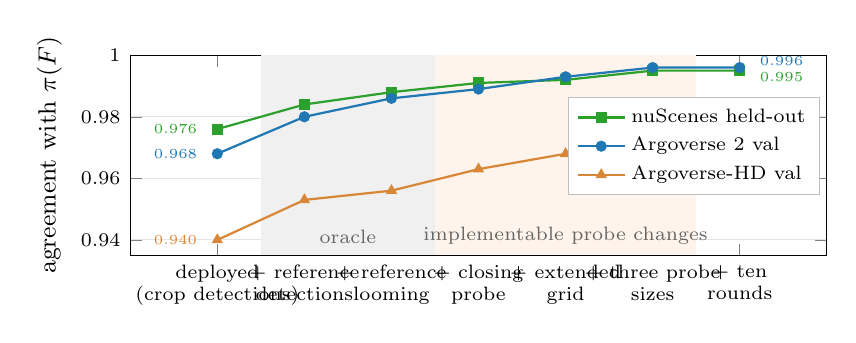
\begin{tikzpicture}
\begin{axis}[width=0.86\linewidth, height=0.34\linewidth, ymin=0.935, ymax=1.0,
  xmin=-1.0, xmax=7.0, xtick={0,...,6}, xticklabels={{deployed\\(crop detections)},{+ reference\\detections},{+ reference\\looming},{+ closing\\probe},{+ extended\\grid},{+ three probe\\sizes},{+ ten\\rounds}},
  xticklabel style={font=\scriptsize, align=center}, yticklabel style={font=\scriptsize,
  /pgf/number format/fixed, /pgf/number format/precision=2}, ylabel={agreement with $\policy(\full)$},
  label style={font=\small}, ymajorgrids, grid style={gray!20},
  legend style={font=\scriptsize, at={(0.99,0.30)}, anchor=south east, draw=gray!50}, legend cell align=left]
\fill[gray!12] (axis cs:0.5,0.935) rectangle (axis cs:2.5,1.0);
\fill[fieldc!10] (axis cs:2.5,0.935) rectangle (axis cs:5.5,1.0);
\node[font=\scriptsize, text=black!60, anchor=south] at (axis cs:1.5,0.9355) {oracle};
\node[font=\scriptsize, text=black!60, anchor=south] at (axis cs:4,0.9355) {implementable probe changes};
\addplot[cropc, thick, mark=square*, mark size=1.6pt] coordinates {(0,0.976) (1,0.984) (2,0.988) (3,0.991) (4,0.992) (5,0.995) (6,0.995)};
\addlegendentry{nuScenes held-out}
\node[font=\tiny, text=cropc, anchor=east] at (axis cs:-0.12,0.976) {0.976};
\node[font=\tiny, text=cropc, anchor=west] at (axis cs:6.12,0.9928) {0.995};
\addplot[adac, thick, mark=*, mark size=1.6pt] coordinates {(0,0.968) (1,0.980) (2,0.986) (3,0.989) (4,0.993) (5,0.996) (6,0.996)};
\addlegendentry{Argoverse~2 val}
\node[font=\tiny, text=adac, anchor=east] at (axis cs:-0.12,0.968) {0.968};
\node[font=\tiny, text=adac, anchor=west] at (axis cs:6.12,0.9982) {0.996};
\addplot[fieldc!90!black, thick, mark=triangle*, mark size=1.6pt] coordinates {(0,0.940) (1,0.953) (2,0.956) (3,0.963) (4,0.968) (5,0.971) (6,0.971)};
\addlegendentry{Argoverse-HD val}
\node[font=\tiny, text=fieldc!90!black, anchor=east] at (axis cs:-0.12,0.940) {0.940};
\node[font=\tiny, text=fieldc!90!black, anchor=west] at (axis cs:6.12,0.9710) {0.971};
\end{axis}
\end{tikzpicture}
\caption{\textbf{Which approximation causes the remaining disagreement with $\policy(\full)$?} Agreement of \method (without refiner) with whole-frame inference at the verification resolution, as the approximations are removed cumulatively from left to right (test splits). Grey: oracle diagnostics, not deployable, that replace the crop detections and their looming estimate by those of the reference; orange: implementable changes of the probe; the last step raises the limit of three rounds to ten. Values in \cref{tab:locality}.}
\label{fig:locality}
\end{figure}

Removed cumulatively, the oracle interventions account for $50\%$, $56\%$, and $26\%$ of the disagreeing frames and the probe changes for most of the remainder, which raises the agreement to $99.5\%$, $99.6\%$, and $97.1\%$; the loop terminates after at most one round in $96\%$, $89\%$, and $86\%$ of the frames.
Applied alone instead of cumulatively, substituting the reference detections inside the crops resolves $42.7\%$, $46.9\%$, and $30.0\%$ of the $218$, $382$, and $897$ disagreeing frames, taking the lift and looming estimate of the matching reference detection $30.3\%$, $54.5\%$, and $30.8\%$, the closing probe $20.2\%$, $19.4\%$, and $19.3\%$ (identical at $10$ and $20$\,m/s), the extended grid $23.9\%$, $27.7\%$, and $15.8\%$, the three probe templates $22.9\%$, $21.5\%$, and $12.8\%$, and ten rounds none.
Each change of the probe also creates $4$ to $111$ new disagreements, and $26.6\%$, $19.9\%$, and $42.4\%$ of the frames are resolved by no single intervention; the causes therefore overlap, most on Argoverse-HD.

\noindent\textbf{Crops outside the verified region.}
As a random-crop diagnostic of whether computation outside the field and the support changes the action (it cannot show that no region outside does), random crops with the sizes of the draft boxes are added strictly outside every verified crop and the field footprint, at $25\%$ and $50\%$ more crop pixels than \method on each frame (five seeds), and processed like the crops of \method without a looming history.
They change the action on $0.009\%$, $0.015$--$0.024\%$, and $0.044$--$0.072\%$ of the frames (mean over seeds), compared with the disagreement of $2.4\%$, $3.2\%$, and $6.0\%$ between the deployed procedure and $\policy(\full)$, and the decision value by $-0.0002$, $-0.0005$ to $-0.0007$, and $-0.0012$ to $-0.0018$; most changes on Argoverse-HD stem from annotated objects outside the field.
In the frames that remain, the annotated scene supports the action of \method in $44$, $34$, and $398$ frames and the action of whole-frame inference in $5$, $5$, and $2$.

% --- Table: disagreement taxonomy (handoff/K30/v3_taxonomy.csv; F = u960 + C1, with the refiner where the pipeline has it) ---
\begin{table}[!tbp]
\centering
\caption{\textbf{Disagreements with whole-frame inference} at the verification resolution with the learned looming estimate and without the refiner ($\full$); each pipeline uses the refiner if it has one. ``Disagr.'': share of frames; ``Pipeline'' / ``$\full$'': share of the disagreeing frames in which the action equals the one required by the annotated scene; ``Crit.'': share of frames in which braking is required and the pipeline takes a lower action than $\full$.}
\label{tab:taxonomy}
\small
\setlength{\tabcolsep}{3pt}
\begin{tabular}{@{}lcccc@{}}
\toprule
Pipeline & Disagr. & Pipeline & $\full$ & Crit. \\
\midrule
\multicolumn{5}{@{}l}{\emph{nuScenes held-out}} \\
Cheap (u320) & 7.0\% & 31\% & 64\% & 1.1\% \\
Native + comp. & 3.8\% & 70\% & 26\% & 0.7\% \\
\oursrow \textbf{\method} & 3.7\% & 70\% & 27\% & 0.9\% \\
\midrule
\multicolumn{5}{@{}l}{\emph{Argoverse~2 val}} \\
Cheap (u320) & 16.0\% & 28\% & 63\% & 1.8\% \\
Native + comp. & 13.1\% & 78\% & 17\% & 3.4\% \\
\oursrow \textbf{\method} & 12.5\% & 81\% & 14\% & 3.5\% \\
\midrule
\multicolumn{5}{@{}l}{\emph{Argoverse-HD val}} \\
Cheap (u320) & 23.0\% & 21\% & 62\% & 4.6\% \\
Native + comp. & 17.2\% & 66\% & 22\% & 5.2\% \\
\oursrow \textbf{\method} & 16.0\% & 73\% & 21\% & 5.1\% \\
\bottomrule
\end{tabular}
\end{table}

\noindent\textbf{Disagreements of the deployed system.}
Without any refiner, the agreement with $\policy(\full)$ is $97.6\%$, $96.8\%$, and $94.0\%$ for \method, $93.0\%$, $84.0\%$, and $77.0\%$ for the cheap detector, and $97.4\%$, $95.1\%$, and $92.2\%$ for native-resolution inference with the learned looming estimate; with the refiner in both \method and $\full$, it is $98.0\%$, $96.9\%$, and $94.2\%$ for \method and $97.7\%$, $95.8\%$, and $92.6\%$ for native-resolution inference.
\Cref{tab:taxonomy} compares the actions of the deployed system with those of $\full$, without any intervention.
In the disagreeing frames, the action of \method equals the required action in $70\%$, $81\%$, and $73\%$ of the cases, and native-resolution inference with the same components behaves alike.
Without any refiner, in the frames in which \method and $\policy(\full)$ disagree, the annotated scene requires the action of \method in $128$, $219$, and $722$ frames, that of $\policy(\full)$ in $81$, $126$, and $130$, and neither in $9$, $37$, and $45$.
Among the $60$ costliest frames in which \method brakes less than required, the decisive object is detected but its time-to-collision, lateral position, or range is estimated inaccurately in $46$, it lies in a crop but is missed in $11$, and it lies outside every crop in $3$; the residual safety-critical errors thus stem from the monocular lift rather than from the selection of the regions.

% --- Table: fidelity with the lift in every row and in F (review/cvpr_final_2026-11-10/fid_v3a: k39_6_fidelity.py on the stored actions with |none -> |v3a) ---
\begin{table}[!htbp]
\centering
\caption{\textbf{Fidelity to the reference action $\policy(\full)$ with the shared lift}, \ie, with the range refiner in every pipeline and in $\full$ (the convention of the main paper; test splits, braking controller, own history, computed from stored actions without the decision loss). A: share of frames with the action of $\policy(\full)$; Rep.: the same on the frames in which the cheap detector differs from $\policy(\full)$ ($671$, $2{,}245$, and $4{,}006$ frames); Trans.: the same on the frames in which $\policy(\full)$ changes from the previous frame; px: detector-input pixels in \% of the native frame, including the guard. Capped: nominal per-frame cap at the pixels of \method. $^{\dagger}$ / $^{*}$: \method significantly higher / lower (paired unit bootstrap, $95\%$).}
\label{tab:fidelity_lift}
\scriptsize
\setlength{\tabcolsep}{2.2pt}
\begin{tabular}{@{}lcccccccccccccc@{}}
\toprule
 & \multicolumn{4}{c}{nuScenes held-out} & & \multicolumn{4}{c}{Argoverse~2 val} & & \multicolumn{4}{c}{Argoverse-HD val} \\
\cmidrule(lr){2-5}\cmidrule(lr){7-10}\cmidrule(l){12-15}
Pipeline & A & Rep. & Trans. & px & & A & Rep. & Trans. & px & & A & Rep. & Trans. & px \\
\midrule
Always \textsc{keep} & 0.911 & 0.580 & 0.429 & 0.0 &  & 0.745 & 0.625 & 0.366 & 0.0 &  & 0.679 & 0.495 & 0.385 & 0.0 \\
u320 & 0.927$^{\dagger}$ & 0.000$^{\dagger}$ & 0.653$^{\dagger}$ & 4.3 &  & 0.810$^{\dagger}$ & 0.000$^{\dagger}$ & 0.555$^{\dagger}$ & 2.6 &  & 0.733$^{\dagger}$ & 0.000$^{\dagger}$ & 0.497$^{\dagger}$ & 3.1 \\
\midrule
Whole frame u512 & 0.978 & 0.800 & 0.763 & 10.2 &  & 0.963$^{\dagger}$ & 0.875 & 0.766 & 6.7 &  & 0.950 & 0.868 & 0.608 & 7.1 \\
Whole frame u640 & 0.983 & 0.861$^{*}$ & 0.827$^{*}$ & 17.1 &  & 0.969 & 0.893 & 0.798 & 10.3 &  & 0.963 & 0.902 & 0.671 & 11.6 \\
Whole frame u1280 & 0.984$^{*}$ & 0.887$^{*}$ & 0.845$^{*}$ & 65.4 &  & 0.976$^{*}$ & 0.931$^{*}$ & 0.843$^{*}$ & 40.0 &  & 0.965 & 0.930$^{*}$ & 0.664 & 44.4 \\
Whole frame native & 0.977 & 0.821 & 0.782 & 103.1 &  & 0.958$^{\dagger}$ & 0.887 & 0.778 & 101.2 &  & 0.925$^{\dagger}$ & 0.869$^{*}$ & 0.633 & 101.3 \\
\midrule
AnA-style, iterated & 0.985$^{*}$ & 0.845$^{*}$ & 0.838$^{*}$ & 10.5 &  & 0.973$^{*}$ & 0.904 & 0.796 & 7.9 &  & 0.967 & 0.913 & 0.683 & 20.6 \\
AdaScale & 0.985$^{*}$ & 0.879$^{*}$ & 0.850$^{*}$ & 30.6 &  & 0.990$^{*}$ & 0.967$^{*}$ & 0.927$^{*}$ & 26.8 &  & 0.985$^{*}$ & 0.965$^{*}$ & 0.866$^{*}$ & 29.9 \\
SAHI & 0.974$^{\dagger}$ & 0.861$^{*}$ & 0.822$^{*}$ & 187.7 &  & 0.928$^{\dagger}$ & 0.799$^{\dagger}$ & 0.737$^{\dagger}$ & 165.2 &  & 0.921 & 0.855 & 0.637 & 153.8 \\
FOVEA, instance saliency & 0.980 & 0.848$^{*}$ & 0.834$^{*}$ & 69.7 &  & 0.958$^{\dagger}$ & 0.893 & 0.791 & 42.6 &  & 0.960 & 0.907 & 0.633 & 47.6 \\
UFP & 0.980 & 0.829 & 0.803 & 18.1 &  & 0.972 & 0.904 & 0.820$^{*}$ & 9.0 &  & 0.957 & 0.884 & 0.683 & 12.8 \\
\midrule
AnA-style, iterated, capped & 0.979 & 0.770 & 0.780 & 5.8 &  & 0.964$^{\dagger}$ & 0.867$^{\dagger}$ & 0.758$^{\dagger}$ & 5.0 &  & 0.936$^{\dagger}$ & 0.814$^{\dagger}$ & 0.649 & 7.4 \\
Counterfactual, iterated, capped & 0.973$^{\dagger}$ & 0.697$^{\dagger}$ & 0.742$^{\dagger}$ & 5.2 &  & 0.961$^{\dagger}$ & 0.841$^{\dagger}$ & 0.739$^{\dagger}$ & 4.2 &  & 0.906$^{\dagger}$ & 0.693$^{\dagger}$ & 0.608 & 5.9 \\
AdaScale, capped & 0.972$^{\dagger}$ & 0.693$^{\dagger}$ & 0.749 & 5.5 &  & 0.950$^{\dagger}$ & 0.804$^{\dagger}$ & 0.716$^{\dagger}$ & 3.7 &  & 0.916 & 0.730 & 0.603 & 5.1 \\
SAHI, capped & 0.945$^{\dagger}$ & 0.697$^{\dagger}$ & 0.686$^{\dagger}$ & 6.4 &  & 0.879$^{\dagger}$ & 0.689$^{\dagger}$ & 0.624$^{\dagger}$ & 4.2 &  & 0.867$^{\dagger}$ & 0.685$^{\dagger}$ & 0.558$^{\dagger}$ & 5.5 \\
FOVEA, instance saliency, capped & 0.962$^{\dagger}$ & 0.745 & 0.726 & 7.5 &  & 0.934$^{\dagger}$ & 0.816$^{\dagger}$ & 0.686$^{\dagger}$ & 5.1 &  & 0.858$^{\dagger}$ & 0.655 & 0.556 & 6.8 \\
UFP, capped & 0.980 & 0.803 & 0.782 & 7.2 &  & 0.958$^{\dagger}$ & 0.855$^{\dagger}$ & 0.757 & 4.8 &  & 0.945 & 0.850 & 0.658 & 6.3 \\
Chanakya-style, capped & 0.933$^{\dagger}$ & 0.088$^{\dagger}$ & 0.691$^{\dagger}$ & 4.6 &  & 0.819$^{\dagger}$ & 0.052$^{\dagger}$ & 0.574$^{\dagger}$ & 2.9 &  & 0.748$^{\dagger}$ & 0.059$^{\dagger}$ & 0.517$^{\dagger}$ & 3.8 \\
\midrule
Support + fixed tube & 0.978 & 0.773 & 0.770 & 10.8 &  & 0.969 & 0.891 & 0.784 & 7.1 &  & 0.942 & 0.838 & 0.644 & 10.8 \\
Support + fixed tube, strict cap & 0.973$^{\dagger}$ & 0.736$^{\dagger}$ & 0.754 & 7.5 &  & 0.963$^{\dagger}$ & 0.872$^{\dagger}$ & 0.773 & 5.1 &  & 0.918$^{\dagger}$ & 0.774$^{\dagger}$ & 0.608$^{\dagger}$ & 6.8 \\
Support only & 0.972$^{\dagger}$ & 0.681$^{\dagger}$ & 0.726$^{\dagger}$ & 5.0 &  & 0.958$^{\dagger}$ & 0.828$^{\dagger}$ & 0.724$^{\dagger}$ & 4.1 &  & 0.905$^{\dagger}$ & 0.691$^{\dagger}$ & 0.599$^{\dagger}$ & 5.6 \\
Field only & 0.943$^{\dagger}$ & 0.244$^{\dagger}$ & 0.700$^{\dagger}$ & 6.8 &  & 0.839$^{\dagger}$ & 0.173$^{\dagger}$ & 0.615$^{\dagger}$ & 3.7 &  & 0.780$^{\dagger}$ & 0.192$^{\dagger}$ & 0.533$^{\dagger}$ & 4.3 \\
\midrule
\oursrow \textbf{\method} & 0.980 & 0.788 & 0.773 & 7.8 &  & 0.969 & 0.892 & 0.790 & 5.4 &  & 0.942 & 0.835 & 0.637 & 7.0 \\
\bottomrule
\end{tabular}
\end{table}

% --- Table: fidelity without the range refiner (handoff/K39/k39_6_fidelity.csv, k39_6_diffs.csv, k39_6_checks.json; reproduced in review/cvpr_final_2026-11-10/fid_none) ---
\begin{table}[!htbp]
\centering
\caption{\textbf{Diagnostic: fidelity without the range refiner} in any pipeline or in $\full$, which isolates the loop that Theorem~\mrefnum{thm:exact} covers. Columns and marks as in \cref{tab:fidelity_lift}; the cheap detector differs from $\policy(\full)$ on $639$, $1{,}891$, and $3{,}447$ frames.}
\label{tab:fidelity}
\scriptsize
\setlength{\tabcolsep}{2.2pt}
\begin{tabular}{@{}lcccccccccccccc@{}}
\toprule
 & \multicolumn{4}{c}{nuScenes held-out} & & \multicolumn{4}{c}{Argoverse~2 val} & & \multicolumn{4}{c}{Argoverse-HD val} \\
\cmidrule(lr){2-5}\cmidrule(lr){7-10}\cmidrule(l){12-15}
Pipeline & A & Rep. & Trans. & px & & A & Rep. & Trans. & px & & A & Rep. & Trans. & px \\
\midrule
Always \textsc{keep} & 0.899 & 0.534 & 0.441 & 0.0 &  & 0.662 & 0.417 & 0.372 & 0.0 &  & 0.592 & 0.293 & 0.363 & 0.0 \\
u320 & 0.930$^{\dagger}$ & 0.000$^{\dagger}$ & 0.657$^{\dagger}$ & 4.3 &  & 0.840$^{\dagger}$ & 0.000$^{\dagger}$ & 0.642$^{\dagger}$ & 2.6 &  & 0.770$^{\dagger}$ & 0.000$^{\dagger}$ & 0.498$^{\dagger}$ & 3.1 \\
\midrule
Whole frame u512 & 0.971$^{\dagger}$ & 0.729 & 0.761 & 10.2 &  & 0.953$^{\dagger}$ & 0.801$^{\dagger}$ & 0.781$^{\dagger}$ & 6.7 &  & 0.942 & 0.831 & 0.609 & 7.1 \\
Whole frame u640 & 0.979 & 0.817$^{*}$ & 0.822$^{*}$ & 17.1 &  & 0.964 & 0.850 & 0.826 & 10.3 &  & 0.958 & 0.884 & 0.662 & 11.6 \\
Whole frame u1280 & 0.982$^{*}$ & 0.873$^{*}$ & 0.856$^{*}$ & 65.4 &  & 0.974$^{*}$ & 0.922$^{*}$ & 0.863$^{*}$ & 40.0 &  & 0.964$^{*}$ & 0.919$^{*}$ & 0.676 & 44.4 \\
Whole frame native & 0.974 & 0.806$^{*}$ & 0.795 & 103.1 &  & 0.951$^{\dagger}$ & 0.882 & 0.800 & 101.2 &  & 0.922$^{\dagger}$ & 0.849$^{*}$ & 0.625 & 101.3 \\
\midrule
AnA-style, iterated & 0.981$^{*}$ & 0.786$^{*}$ & 0.822$^{*}$ & 10.5 &  & 0.963 & 0.828$^{\dagger}$ & 0.815 & 7.9 &  & 0.960 & 0.870 & 0.672 & 20.6 \\
AdaScale & 0.981$^{*}$ & 0.829$^{*}$ & 0.820$^{*}$ & 30.6 &  & 0.986$^{*}$ & 0.944$^{*}$ & 0.923$^{*}$ & 26.8 &  & 0.985$^{*}$ & 0.963$^{*}$ & 0.850$^{*}$ & 29.9 \\
SAHI & 0.967$^{\dagger}$ & 0.822$^{*}$ & 0.816$^{*}$ & 187.7 &  & 0.918$^{\dagger}$ & 0.824$^{\dagger}$ & 0.783$^{\dagger}$ & 165.2 &  & 0.920 & 0.890 & 0.631 & 153.8 \\
FOVEA, instance saliency & 0.976 & 0.825$^{*}$ & 0.824$^{*}$ & 69.7 &  & 0.951$^{\dagger}$ & 0.854 & 0.818 & 42.6 &  & 0.956 & 0.885 & 0.648 & 47.6 \\
UFP & 0.975 & 0.765 & 0.786 & 18.1 &  & 0.957$^{\dagger}$ & 0.807$^{\dagger}$ & 0.816 & 9.0 &  & 0.953 & 0.856 & 0.668 & 12.8 \\
\midrule
AnA-style, iterated, capped & 0.974 & 0.704$^{\dagger}$ & 0.771 & 5.8 &  & 0.955$^{\dagger}$ & 0.786$^{\dagger}$ & 0.787$^{\dagger}$ & 5.0 &  & 0.932$^{\dagger}$ & 0.766$^{\dagger}$ & 0.633 & 7.4 \\
Counterfactual, iterated, capped & 0.966$^{\dagger}$ & 0.585$^{\dagger}$ & 0.712$^{\dagger}$ & 5.2 &  & 0.934$^{\dagger}$ & 0.644$^{\dagger}$ & 0.753$^{\dagger}$ & 4.2 &  & 0.890$^{\dagger}$ & 0.573$^{\dagger}$ & 0.596 & 5.9 \\
AdaScale, capped & 0.967$^{\dagger}$ & 0.585$^{\dagger}$ & 0.731 & 5.5 &  & 0.928$^{\dagger}$ & 0.595$^{\dagger}$ & 0.732$^{\dagger}$ & 3.7 &  & 0.908 & 0.623 & 0.592 & 5.1 \\
SAHI, capped & 0.936$^{\dagger}$ & 0.604$^{\dagger}$ & 0.665$^{\dagger}$ & 6.4 &  & 0.840$^{\dagger}$ & 0.529$^{\dagger}$ & 0.598$^{\dagger}$ & 4.2 &  & 0.851$^{\dagger}$ & 0.616$^{\dagger}$ & 0.549$^{\dagger}$ & 5.5 \\
FOVEA, instance saliency, capped & 0.955$^{\dagger}$ & 0.673 & 0.720$^{\dagger}$ & 7.5 &  & 0.911$^{\dagger}$ & 0.675$^{\dagger}$ & 0.729$^{\dagger}$ & 5.1 &  & 0.842$^{\dagger}$ & 0.602 & 0.537$^{\dagger}$ & 6.8 \\
UFP, capped & 0.973 & 0.725 & 0.756 & 7.2 &  & 0.937$^{\dagger}$ & 0.738$^{\dagger}$ & 0.766$^{\dagger}$ & 4.8 &  & 0.936 & 0.801 & 0.641 & 6.3 \\
Chanakya-style, capped & 0.936$^{\dagger}$ & 0.085$^{\dagger}$ & 0.688$^{\dagger}$ & 4.6 &  & 0.847$^{\dagger}$ & 0.045$^{\dagger}$ & 0.652$^{\dagger}$ & 2.9 &  & 0.787$^{\dagger}$ & 0.076$^{\dagger}$ & 0.512$^{\dagger}$ & 3.8 \\
\midrule
Support + fixed tube & 0.974$^{\dagger}$ & 0.718 & 0.767 & 10.8 &  & 0.967 & 0.868 & 0.821 & 7.1 &  & 0.939 & 0.803 & 0.645 & 10.8 \\
Support + fixed tube, strict cap & 0.969$^{\dagger}$ & 0.681$^{\dagger}$ & 0.750 & 7.5 &  & 0.962$^{\dagger}$ & 0.850$^{\dagger}$ & 0.813 & 5.1 &  & 0.924$^{\dagger}$ & 0.753$^{\dagger}$ & 0.633 & 6.8 \\
Support only & 0.964$^{\dagger}$ & 0.563$^{\dagger}$ & 0.701$^{\dagger}$ & 5.0 &  & 0.929$^{\dagger}$ & 0.617$^{\dagger}$ & 0.732$^{\dagger}$ & 4.1 &  & 0.888$^{\dagger}$ & 0.562$^{\dagger}$ & 0.578$^{\dagger}$ & 5.6 \\
Field only & 0.944$^{\dagger}$ & 0.225$^{\dagger}$ & 0.720$^{\dagger}$ & 6.8 &  & 0.880$^{\dagger}$ & 0.283$^{\dagger}$ & 0.733$^{\dagger}$ & 3.7 &  & 0.822$^{\dagger}$ & 0.247$^{\dagger}$ & 0.568$^{\dagger}$ & 4.3 \\
\midrule
\oursrow \textbf{\method} & 0.976 & 0.734 & 0.769 & 7.8 &  & 0.968 & 0.870 & 0.822 & 5.4 &  & 0.940 & 0.803 & 0.643 & 7.0 \\
\bottomrule
\end{tabular}
\end{table}

\noindent\textbf{Fidelity with the shared lift.}
\Cref{tab:fidelity_lift} states the fidelity in the convention of the main paper: every pipeline and the reference $\full$ use the lift, including the range refiner.
\method agrees with $\policy(\full)$ on $98.0\%$, $96.9\%$, and $94.2\%$ of the frames and repairs $78.8\%$, $89.2\%$, and $83.5\%$ of the disagreements of the cheap detector.
Under the nominal cap, it repairs significantly more than the published, learned, and object-level methods in $27$ of the $36$ comparisons and significantly less in none (the nine others: AnA-style refinement, FOVEA, and UFP on nuScenes, and AdaScale, FOVEA, and UFP on Argoverse-HD); under the strict cap, it repairs significantly more than the hybrid and the primary crop heuristics in all $12$ comparisons.
Whole-frame inference at $512$ pixels, with $1.0$--$1.3\times$ the pixels of \method, repairs $80.0\%$, $87.5\%$, and $86.8\%$, which does not differ significantly on any dataset; its raw agreement is significantly lower only on Argoverse~2.
At similar pixels, a lower whole-frame resolution is therefore as faithful to the reference as \method; the two differ in decision value (\cref{tab:uniform}) and in latency (\cref{tab:latency}).
At changes of $\policy(\full)$, \method agrees on $77.3\%$, $79.0\%$, and $63.7\%$ of the frames, and on the frames in which it differs from $\policy(\full)$, the annotated scene requires its action in $58\%$, $55\%$, and $81\%$ and that of $\policy(\full)$ in $38\%$, $37\%$, and $15\%$.

\noindent\textbf{Fidelity without the range refiner.}
The raw agreement is dominated by \textsc{keep}: without the refiner, always keeping the speed agrees with $\policy(\full)$ on $89.9\%$, $66.2\%$, and $59.2\%$ of the frames.
\Cref{tab:fidelity} therefore also reports the repair rate, \ie, the agreement on the frames in which the draft differs from $\policy(\full)$, and the agreement at changes of $\policy(\full)$; both are computed from stored actions, without any detector run and without the decision loss.
\method repairs $73.4\%$, $87.0\%$, and $80.3\%$ of the disagreements of the draft.
Under the nominal cap, it repairs significantly more than the published, learned, and object-level methods in $29$ of the $36$ comparisons and significantly less in none; under the strict cap, it repairs significantly more than the hybrid and the primary crop heuristics in all $12$ comparisons.
Under the nominal cap of \mref{tab:planners}, with $1.3$--$1.5\times$ the pixels, the hybrid ties \method in repair rate on all three datasets.
Every pipeline that repairs significantly more uses more pixels: iterated AnA-style refinement on nuScenes ($1.3\times$), whole-frame inference from $640$ pixels on nuScenes ($2.2\times$) and at $1280$ pixels elsewhere ($6$--$8\times$), AdaScale ($4$--$5\times$), and SAHI and FOVEA on nuScenes ($9$--$24\times$).
\Cref{fig:fidelity} plots the repair rate against the pixels.
At the same pixels on Argoverse-HD, whole-frame inference at $512$ pixels repairs $83.1\%$ (not significant), and \method is significantly more faithful only when braking is required ($95.4\%$ \vs $89.7\%$).
The agreement at changes of $\policy(\full)$ is the weakest metric of \method ($76.9\%$, $82.2\%$, and $64.3\%$): when the set of crops changes, the history of an object detected in a crop starts anew.
On the frames in which \method differs from $\policy(\full)$, the annotated scene requires its action in $59\%$, $57\%$, and $80\%$ and that of $\policy(\full)$ in $37\%$, $33\%$, and $14\%$; for whole-frame inference at $1280$ pixels and for AdaScale, the two shares lie within $11$ points of each other.

% --- Fig.: repair rate vs pixels (handoff/K39/k39_6_fidelity.csv; every pipeline without refiner; u960 = target omitted) ---
\begin{figure}[!htbp]
\centering
\begin{minipage}{0.52\linewidth}\centering
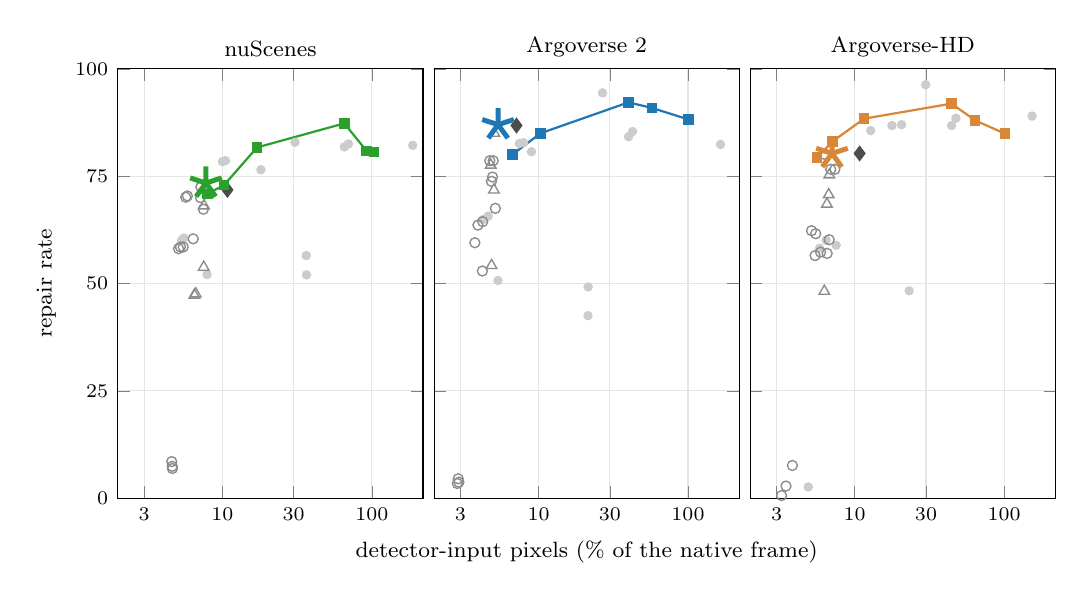
\begin{tikzpicture}
\begin{groupplot}[group style={group size=3 by 1, horizontal sep=4pt, yticklabels at=edge left},
width=0.45\linewidth, height=0.58\linewidth, scale only axis=false,
xmode=log, xmin=0.02, xmax=2.2, ymin=0, ymax=1.0, xtick={0.03,0.1,0.3,1}, xticklabels={3,10,30,100},
ytick={0,0.25,0.5,0.75,1}, yticklabels={0,25,50,75,100},
tick label style={font=\scriptsize}, label style={font=\footnotesize}, title style={font=\footnotesize, yshift=-5pt},
grid=major, grid style={gray!20}, xlabel style={font=\footnotesize}]
\nextgroupplot[title={nuScenes}, ylabel={repair rate}]
\addplot[gray!40, only marks, mark=*, mark size=1.5pt] coordinates {(0.1002,0.784) (0.1047,0.786) (0.0534,0.601) (0.0553,0.606) (0.3059,0.829) (1.8773,0.822) (0.6969,0.825) (0.6542,0.818) (0.1810,0.765) (0.3655,0.520) (0.3641,0.565) (0.0790,0.521)};
\label{fid:unc}
\addplot[black!45, only marks, mark=o, mark size=1.8pt, line width=0.5pt] coordinates {(0.0569,0.701) (0.0583,0.704) (0.0509,0.581) (0.0524,0.585) (0.0547,0.585) (0.0638,0.604) (0.0746,0.673) (0.0713,0.700) (0.0718,0.725) (0.0463,0.069) (0.0462,0.074) (0.0458,0.085)};
\label{fid:cap}
\addplot[black!45, only marks, mark=triangle, mark size=2.2pt, line width=0.5pt] coordinates {(0.0649,0.473) (0.0663,0.476) (0.0750,0.538) (0.0754,0.681)};
\label{fid:strict}
\addplot[black!70, only marks, mark=diamond*, mark size=2.6pt] coordinates {(0.1081,0.718)};
\label{fid:hyb}
\addplot[cropc, thick, mark=square*, mark size=1.5pt] coordinates {(0.0796,0.709) (0.1024,0.729) (0.1707,0.817) (0.6542,0.873) (0.9216,0.809) (1.0311,0.806)};
\label{fid:wf}
\addplot[cropc, only marks, mark=star, mark size=6pt, line width=1.8pt] coordinates {(0.0776,0.734)};
\label{fid:ours}
\nextgroupplot[title={Argoverse~2}]
\addplot[gray!40, only marks, mark=*, mark size=1.5pt] coordinates {(0.0744,0.826) (0.0794,0.828) (0.0425,0.649) (0.0460,0.657) (0.2679,0.944) (1.6516,0.824) (0.4258,0.854) (0.4000,0.842) (0.0897,0.807) (0.2142,0.425) (0.2147,0.492) (0.0535,0.507)};
\addplot[black!45, only marks, mark=o, mark size=1.8pt, line width=0.5pt] coordinates {(0.0472,0.786) (0.0497,0.786) (0.0393,0.636) (0.0423,0.644) (0.0375,0.595) (0.0421,0.529) (0.0514,0.675) (0.0492,0.748) (0.0484,0.738) (0.0286,0.034) (0.0293,0.037) (0.0290,0.045)};
\addplot[black!45, only marks, mark=triangle, mark size=2.2pt, line width=0.5pt] coordinates {(0.0485,0.542) (0.0503,0.718) (0.0479,0.776) (0.0506,0.850)};
\addplot[black!70, only marks, mark=diamond*, mark size=2.6pt] coordinates {(0.0712,0.868)};
\addplot[adac, thick, mark=square*, mark size=1.5pt] coordinates {(0.0671,0.801) (0.1032,0.850) (0.4000,0.922) (0.5729,0.909) (1.0116,0.882)};
\addplot[adac, only marks, mark=star, mark size=6pt, line width=1.8pt] coordinates {(0.0536,0.870)};
\nextgroupplot[title={Argoverse-HD}]
\addplot[gray!40, only marks, mark=*, mark size=1.5pt] coordinates {(0.1776,0.868) (0.2058,0.870) (0.0582,0.582) (0.0643,0.601) (0.2986,0.963) (1.5378,0.890) (0.4756,0.885) (0.4444,0.868) (0.1280,0.856) (0.2313,0.483) (0.0489,0.026) (0.0752,0.589)};
\addplot[black!45, only marks, mark=o, mark size=1.8pt, line width=0.5pt] coordinates {(0.0691,0.766) (0.0737,0.766) (0.0543,0.565) (0.0591,0.573) (0.0514,0.623) (0.0548,0.616) (0.0675,0.602) (0.0654,0.570) (0.0627,0.801) (0.0347,0.028) (0.0324,0.006) (0.0383,0.076)};
\addplot[black!45, only marks, mark=triangle, mark size=2.2pt, line width=0.5pt] coordinates {(0.0626,0.482) (0.0670,0.707) (0.0652,0.685) (0.0676,0.753)};
\addplot[black!70, only marks, mark=diamond*, mark size=2.6pt] coordinates {(0.1079,0.803)};
\addplot[fieldc!90!black, thick, mark=square*, mark size=1.5pt] coordinates {(0.0560,0.793) (0.0711,0.831) (0.1156,0.884) (0.4444,0.919) (0.6400,0.880) (1.0133,0.849)};
\addplot[fieldc!90!black, only marks, mark=star, mark size=6pt, line width=1.8pt] coordinates {(0.0705,0.803)};
\end{groupplot}
\node[font=\footnotesize, anchor=north] at ($(group c2r1.south)+(0,-0.42)$) {detector-input pixels (\% of the native frame)};
\end{tikzpicture}\\[1pt]
{\footnotesize\setlength{\tabcolsep}{4pt}\begin{tabular}{@{}lll@{}}\ref{fid:ours}~\method & \ref{fid:wf}~whole frame & \ref{fid:hyb}~hybrid \\ \ref{fid:unc}~methods, no cap & \ref{fid:cap}~methods, nominal cap & \ref{fid:strict}~strict cap\end{tabular}}
\end{minipage}
\caption{\textbf{Repair rate \vs pixels}, without the refiner. Share of the cheap detector's disagreements with $\policy(\full)$ that a pipeline resolves (u960, the reference, omitted; values in \cref{tab:fidelity}). \method lies on the upper-left frontier of the tested pipelines: every pipeline above it uses more pixels.}
\label{fig:fidelity}
\end{figure}

% --- K40-1 (handoff/K40R/k40_1_target.csv, k40_1_decomposition.csv; pre-specified post-hoc) ---
\noindent\textbf{Fidelity and decision value.}\label{sec:supp_fidelity_G}
Fidelity does not fix the decision value: $\G$ scores the actions against the annotated scene, whereas $\policy(\full)$ is itself the action of a detector.
The reference attains $\G=0.085$ $\ci{-0.203}{+0.347}$, $0.290$ $\ci{0.234}{0.350}$, and $0.296$ $\ci{0.097}{0.462}$ on nuScenes, Argoverse~2, and Argoverse-HD, and \method without the refiner $0.181$, $0.241$, and $0.422$.
The differences, $+0.096$ $\ci{-0.085}{+0.305}$, $-0.049$ $\ci{-0.116}{+0.007}$, and $+0.126$ $\best{\ci{+0.015}{+0.332}}$, arise entirely on the $218$, $382$, and $897$ frames on which the two actions differ: since the previous action in the loss is that of the cheap pipeline for all pipelines (\cref{sec:supp_metric}), every loss term is equal on the other frames, and their contribution is exactly zero.
On the differing frames, \method has less excessive-braking loss on all three datasets ($+0.037$ $\ci{+0.020}{+0.067}$, $+0.029$ $\ci{+0.018}{+0.041}$, and $+0.131$ $\ci{+0.021}{+0.336}$, in units of the loss of the cheap pipeline) and more insufficient-braking loss on Argoverse~2 and Argoverse-HD ($-0.076$ $\ci{-0.143}{-0.023}$ and $-0.007$ $\ci{-0.011}{-0.003}$).
Its higher point estimates on nuScenes and Argoverse-HD therefore come from fewer excessive braking actions on the few frames on which its crops and object histories yield a different scene than whole-frame inference.
With the refiner, the differences to the reference are $+0.125$, $+0.003$, and $+0.122$, none significant.

%%%%%%%%%%%%%%%%%%%%%%%%%%%%%%%%%%%%%%%%%%%%%%%%%%%%%%%%%%%%%%%%%%%%%%%%%%%%%%
%% S2. IMPLEMENTATION, PROTOCOL, AND BASELINE FAIRNESS
%%%%%%%%%%%%%%%%%%%%%%%%%%%%%%%%%%%%%%%%%%%%%%%%%%%%%%%%%%%%%%%%%%%%%%%%%%%%%%
\section{Implementation, evaluation protocol, and baseline fairness}
\label{sec:supp_impl}

This section specifies the planner and the decision value (\cref{sec:supp_metric}), the benchmarks, the configuration, and the selection protocol (\cref{sec:supp_config}), the accounting of detector-input pixels (\cref{sec:supp_pixels}), the ego mask on Argoverse~2 (\cref{sec:supp_hood}), and the baselines and the checks that make their comparison fair (\cref{sec:supp_baselines,sec:supp_fairness}).

\subsection{Planner and decision value}
\label{sec:supp_metric}

For completeness, this section restates the benchmark components of~\cite{deep} that our experiments adopt: the monocular lift, the braking controller, and the loss behind the decision value $\G$. The decision-exactness objective and its measurement by the action agreement with $\policy(\full)$ (\cref{sec:theory_practice}) use the controller but not the loss.

\noindent\textbf{Monocular lifting.}
Each 2D detection is lifted to an object state in the ego frame with a pinhole camera model.
The range is a combination of a ground-plane cue, computed from the bottom edge of the box, and a height cue, computed from the box height and a class-specific height prior. The weight of the ground-plane cue increases with the distance of the contact point from the horizon.
The lateral extent is obtained from the horizontal box edges at the estimated range, and the time-to-collision from the change of the box between consecutive frames.
The ``oracle'' geometry replaces the range of matched boxes by the annotated range; it is used only in diagnostic analyzes, and the deployed pipeline estimates ranges from the image detections.

\noindent\textbf{Braking controller.}
For an object within the ego corridor (half-width $1.2$\,m) and within $80$\,m, at range $r$ and with ego speed $v$, the demand is
\begin{equation}
\dem = \min\!\Big(\max\Big(\tfrac{v^2}{2\,(r-r_0-v\,t_r)},\ \tfrac{v_{\mathrm{rel}}^2}{2\,(r-r_0)}\Big),\ 9\Big)\ \mathrm{m/s^2},
\label{eq:s_demand}
\end{equation}
with stand-off distance $r_0=2$\,m, reaction time $t_r=0.4$\,s, and closing speed $v_{\mathrm{rel}}=r/\mathrm{ttc}$, where the denominators are bounded from below by $0.1$\,m. Objects outside the corridor have $\dem=0$.
The action is \textsc{hard-brake} if the maximum demand is at least $\tau_2=3.5\,\mathrm{m/s^2}$, \textsc{decelerate} if it is at least $\tau_1=1.0\,\mathrm{m/s^2}$, and \textsc{keep} otherwise. The commanded decelerations are $u=6.0$, $2.5$, and $0\,\mathrm{m/s^2}$, respectively.

\noindent\textbf{Loss.}
Let $\dem^\star$ denote the maximum demand over the annotated objects; the object that attains it is the \emph{decisive object} of the frame, and an annotated object is \emph{decision-relevant} if its own demand reaches $\tau_1$.
The loss of action $a$ with command $u(a)$ is
\begin{equation}
L = \lambda_r\,[\dem^\star-u(a)]_+^2 + \lambda_b\,[u(a)-\dem^\star]_+^2
 + \lambda_j\,|u(a)-u(a_{\mathrm{prev}})| + \lambda_c\,\mathbb{1}\big[\dem^\star-u(a)\ge 8\big],
\label{eq:s_loss}
\end{equation}
with $(\lambda_r,\lambda_b,\lambda_j,\lambda_c)=(1,\,0.12,\,0.02,\,6)$.
The previous action $a_{\mathrm{prev}}$ is that of the cheap pipeline for all methods, such that all pipelines are evaluated against the same history.
The loss is asymmetric: insufficient braking is penalized as a safety shortfall, whereas excessive braking costs comfort and progress.

\noindent\textbf{Perception in the loop for planners.}
For NAVSIM and nuPlan, an annotated object that projects into the front camera is retained only if it is matched to a detection (Hungarian matching, compatible class, IoU $\ge0.3$). Unmatched annotated objects within the camera frustum are removed, unmatched detections are converted to static objects on the ground plane with the class-median size, and objects outside the camera frustum remain privileged.

\subsection{Benchmarks, configuration, and selection protocol}
\label{sec:supp_config}


\begin{table}[!htbp]
\centering
\caption{\textbf{Benchmarks and configurations.} Configurations are selected on the development split, and the final configuration is frozen before its evaluation on the test split. The nuScenes development and test splits (the latter is not the official test set) are disjoint sets of $152$ and $228$ scenes of its trainval set, also disjoint from the scenes used for training. Front-camera resolutions: nuScenes $1600\times900$, Argoverse~2 $1550\times2048$, Argoverse-HD $1920\times1200$ at $30$\,Hz. One configuration is used for the three megapixel datasets, KITTI, and Bench2Drive; NAVSIM uses the listed variant for its trajectory planner.}
\label{tab:benchmarks}
\small
\setlength{\tabcolsep}{4pt}
\renewcommand{\arraystretch}{1.15}
\begin{tabular}{@{}p{1.9cm}p{2.2cm}p{3.3cm}lp{4.8cm}p{1.9cm}@{}}
\toprule
Benchmark & Development & Test & Metric & Configuration & Selected on \\
\midrule
nuScenes\newline Argoverse~2\newline Argoverse-HD & 152 scenes\newline train, 700 logs\newline \na & 228 scenes, 9{,}181 fr.\newline val, 150 logs, 11{,}818 fr.\newline val, 24 seq., 15{,}006 fr. & $\G$ & Braking field with a static probe ($\vclose=0$), $\le3$ rounds, crops at $960/\text{long side}$ ($s=0.6$, $0.469$, and $0.5$), truncation guard, scene history with the learned looming estimate, range refiner & nuScenes development split and Argoverse~2 training logs \\
\midrule
KITTI & 15 sequences & 6 seq., 3{,}536 fr. & $\G$ & Configuration of the megapixel datasets & Not tuned \\
NAVSIM & OpenScene mini & navtest, 12{,}146 scenes & PDMS & Field and support obtained by probing PDM-Closed ($7\times7$ grid, $8$--$55$\,m longitudinal, $\pm10.5$\,m lateral; a cell is sensitive if the $4$\,s trajectory moves by more than $0.5$\,m), crop scale $0.5$, one round, guard & OpenScene mini \\
Bench2Drive & \na & 219 routes & DS & Configuration of the megapixel datasets without the refiner, since matched objects retain their true state & Not tuned \\
\bottomrule
\end{tabular}
\end{table}

The grid of the braking field comprises the ranges $\{12.5, 17.5, 22.5, 27.5, 35, 45, 55, 70\}$\,m and lateral offsets from $-6$ to $6$\,m in steps of $1.5$\,m, with a static probe of $1.8\times1.6$\,m; the loop runs at most three rounds, crops at the scale of the frame resized to a long side of $960$ pixels, the truncation guard enlarges a crop at most twice, and each support object contributes a crop of twice its box size around its center.
\emph{Merge rule:} a draft detection is replaced if its box center lies in a verified crop; detections of overlapping crops with IoU $\ge0.5$ keep the more confident one, and a draft detection with IoU $\ge0.5$ to a kept detection is also removed once guard crops were used.
A static probe ($\vclose=0$) carries no closing rate, so that its demand reduces to the first term of~\cref{eq:s_demand}, that of a stationary obstacle.
The sensitivity analyzes also use $\vclose>0$, whose meaning follows the planner: for the braking controller, the probe has the time-to-collision $r/\vclose$, \ie, $\vclose$ is the closing speed of~\cref{eq:s_demand}; for the time-to-collision warning, it has the time-to-collision $r/(v+\vclose)$. Both coincide with a stationary obstacle at $\vclose=0$.

\noindent\textbf{Range refiner.}
The refiner is a ResNet-18~\cite{resnet} that receives a $64\times64$ crop and box features and regresses a correction of the log-range.
It is trained on detections from KITTI train ($14{,}605$), nuScenes training scenes ($62{,}527$), and $340$ Argoverse~2 training logs ($96{,}918$), with model selection on KITTI val and $60$ further Argoverse~2 training logs.
No scene or log of a development or test split and no Argoverse-HD data are used.
On the held-out detections, it reduces the mean absolute log-range error of the lift from $0.263$ to $0.058$.

\noindent\textbf{Looming estimate.}
The looming estimate applies a ResNet-18 with shared weights to the $64\times64$ crops of an object in the last three frames and combines the features with the box features, the ratios of consecutive box heights, and the frame interval.
It regresses the relative closing rate, \ie, the inverse time-to-collision, and an object is assigned a time-to-collision only if the estimated rate exceeds a small threshold.
All three observations must stem from detections at the same scale; an object with fewer observations carries no time-to-collision.
The estimate is trained on detections from the Argoverse~2 training logs of the refiner and from the nuScenes training scenes, with model selection on held-out logs and scenes of both.
It applies to crop detections and, for the baselines that are given the shared components, to whole-frame detections alike.
The hand-crafted alternative in \cref{tab:ablation_impl,tab:versions} takes the median of the pairwise growth estimates over the same three observations.

\noindent\textbf{Protocol.}
The configuration was selected on development data only, namely the nuScenes development split ($152$ scenes) and $300$ Argoverse~2 training logs that are disjoint from the logs used for the refiner and the looming estimate.
A component or parameter was adopted if the interval of its effect was above zero on one development set and its point estimate was not negative on the other, and shared values were preferred over dataset-specific ones.
The configuration, its code, the weights of the refiner and of the looming estimate, and the decision criterion were then frozen before the evaluation on the three test splits; Argoverse-HD was not used for selection.
Every component that distinguishes the final configuration from those in \cref{tab:versions} was selected on the development data.
The parameter grids of the crop heuristics were defined and tuned on the same development data.
The analyzes in \cref*{M-sec:exp_ablation,M-sec:exp_exact} were conducted on the test splits with the final configuration; no configuration was changed on their basis.
The ego mask on Argoverse~2 is a fixed image band (rows $\ge1830$ of 2048) that covers the hood of the ego vehicle; it is applied identically to all pipelines by discarding the detections whose box lies in the band by at least one half (\cref{sec:supp_hood}).

% --- Table: configurations (handoff/K28 phase3/roadmap_v6.csv, seeds_test_v6.csv) ---
\begin{table}[!tbp]
\centering
\caption{\textbf{Configurations evaluated on the test splits} (decision value $\G$; detector-input pixels in \% in parentheses). M and L use a larger detector on the crops.}
\label{tab:versions}
\small
\setlength{\tabcolsep}{2.5pt}
\begin{tabular}{@{}lccc@{}}
\toprule
Configuration & nuScenes & Argoverse 2 & Argov.-HD \\
\midrule
Earlier configuration & 0.170 (10.0) & 0.122 (5.3) & 0.091 (7.0) \\
Hand-crafted looming & 0.199 (7.7) & 0.262 (5.3) & 0.338 (7.0) \\
\oursrow \textbf{\method} & 0.211 (7.8) & 0.294 (5.4) & 0.418 (7.0) \\
\midrule
M: YOLOv8m on the crops & 0.298 (6.5) & 0.281 (4.4) & 0.428 (5.7) \\
L: YOLO11m on the crops & 0.315 (7.7) & 0.292 (5.4) & 0.431 (7.0) \\
\bottomrule
\end{tabular}
\end{table}

\noindent\textbf{Configurations.}
\Cref{tab:versions} lists the configurations that were evaluated on the test splits.
The learned looming estimate improves on the hand-crafted one on all three datasets ($\ci{+0.004}{+0.026}$, $\ci{+0.013}{+0.050}$, and $\ci{+0.054}{+0.107}$), and \method improves on the earlier configuration by $0.041$, $0.171$, and $0.327$ (intervals $\ci{-0.005}{+0.087}$, $\ci{+0.115}{+0.229}$, and $\ci{+0.225}{+0.437}$).
Across three training seeds of the refiner, the standard deviation of $\G$ is $0.002$, $0.005$, and $0.006$.
A larger detector on the crops raises the decision value on nuScenes to $0.298$ and $0.315$.

\subsection{Pixel accounting}
\label{sec:supp_pixels}

The detector-input pixels of \method are measured on the detector input tensors, including the rounding of each crop to a multiple of 32 pixels and the re-detections of the truncation guard.
\method processes no crop in $42\%$, $34\%$, and $27\%$ of the frames on nuScenes, Argoverse~2, and Argoverse-HD and $0.7$, $0.9$, and $1.0$ crops per frame on average; the $95$th percentile of the detector-input pixels per frame is $17.6\%$, $12.9\%$, and $17.5\%$.
In \cref*{M-tab:main}, the detector-input pixels of a method include the cheap pass if the method uses it, the padded mosaics of UFP, and the canvases of FOVEA.
A crop heuristic adds crops in its own order until its budget is reached, and the re-detections of the truncation guard are added on top.
Each heuristic is evaluated at three budgets; at the smallest one, which is used in \cref{tab:heuristics}, the heuristics receive $1.2$ to $2.4\times$ the detector-input pixels of \method, since they issue a larger number of small crops and more guard re-detections.
The $64\times64$ inputs of the range refiner, which amount to less than $0.3\%$ of a frame per support object, and those of the looming estimate are not counted as detector-input pixels; their runtime is included in all latency measurements.

\subsection{Ego mask on Argoverse~2}
\label{sec:supp_hood}

% --- Table: Argoverse 2 without the ego mask (handoff/K28 phase3/ctable_nomask.csv) ---
\begin{table}[!tbp]
\centering
\caption{\textbf{Argoverse~2 val without the ego mask.} ``$\Delta$'' is the $95\%$ interval of (\method$\,-\,$method). All baselines use the refiner; ``+ looming'': and the learned looming estimate. Crop heuristics: best variant at the smallest budget, with both components.}
\label{tab:hood}
\small
\setlength{\tabcolsep}{3pt}
\begin{tabular}{@{}lccc@{}}
\toprule
Method & $\G\uparrow$ & px\,(\%) & $\Delta$ \\
\midrule
u640 & 0.118 & 10.3 & \best{\ci{+0.437}{+0.560}} \\
u960 & 0.496 & 23.2 & \best{\ci{+0.089}{+0.152}} \\
u1280 & 0.534 & 40.0 & \best{\ci{+0.055}{+0.109}} \\
u1536 & 0.609 & 57.3 & \ci{-0.022}{+0.037} \\
Native & 0.639 & 101.2 & \ci{-0.065}{+0.021} \\
u960 + looming & 0.546 & 23.2 & \best{\ci{+0.036}{+0.104}} \\
u1280 + looming & 0.587 & 40.0 & \ci{-0.004}{+0.061} \\
u1536 + looming & 0.669 & 57.3 & \ci{-0.088}{-0.020}\sw \\
Native + looming & 0.693 & 101.2 & \ci{-0.120}{-0.033}\sw \\
\midrule
Uncertainty crops & 0.478 & 10.8 & \best{\ci{+0.108}{+0.173}} \\
Temporal-criticality crops & 0.290 & 10.7 & \best{\ci{+0.294}{+0.361}} \\
Ego-corridor crops & 0.036 & 7.9 & \best{\ci{+0.528}{+0.636}} \\
Support + ego-corridor crops & 0.619 & 8.9 & \ci{-0.008}{+0.003} \\
Random crops & 0.117 & 12.6 & \best{\ci{+0.454}{+0.546}} \\
\midrule
\method w/o refiner & 0.610 & 7.4 & \best{\ci{+0.002}{+0.016}} \\
\oursrow \textbf{\method} & 0.617 & 7.4 & \na \\
\bottomrule
\end{tabular}
\end{table}

The front camera of Argoverse~2 images the hood of the ego vehicle at the bottom of the frame.
At low resolution, the COCO-pretrained detector reports the hood as a vehicle in the ego corridor: it determines the action of the cheap detector in $51\%$ of the frames and accounts for $81\%$ of its decision loss, whereas it rarely affects native-resolution inference ($0.3\%$ of the frames).
Since this spurious object can be removed for every pipeline by a static mask, the main paper reports the results with the mask, and \cref{tab:hood} reports the results without it.
In this setting, the hood detection belongs to the support of the draft action, and \method verifies and removes it without any mask; it attains $\G=0.617$ with $7.4\%$ of the native pixels and significantly outperforms whole-frame inference with the refiner up to a long side of $1280$ pixels, with both components up to $960$ pixels, and the crop heuristics based on uncertainty, temporal criticality, and the ego corridor.
On nuScenes and Argoverse-HD, no part of the ego vehicle is visible, and the corresponding mask changes none of the results.

\subsection{Baselines}
\label{sec:supp_baselines}

\begin{table}[!tbp]
\centering
\caption{\textbf{Baselines, implementations, and fidelity checks.} All baselines use YOLOv8s as the detector unless the official implementation prescribes otherwise. ``Official'': the released code; ``re-implementation'': our implementation of the published method; ``-style'': the objective or selection rule of the cited work adapted to our planner and pipeline, not a reproduction of the original system. \na: no quantitative fidelity check exists for this row.}
\label{tab:baselines}
\small
\begin{tabular}{@{}p{3.0cm}p{5.4cm}p{7.2cm}@{}}
\toprule
Baseline & Implementation & Fidelity check \\
\midrule
AdaScale~\cite{adascale} & Re-implementation (original: Caffe, R-FCN); ResNet-18 scale classifier over $\{320,\dots,960\}$ & \na \\
Budget-Adaptive Routing~\cite{bgtada} & Official estimators, offloader, and arbiter; the decision-value targets are our addition & Official VOC results reproduced within $\pm0.01$ \\
FOVEA~\cite{fovea} & Official grid generator (KDE from the draft detections or from a dataset prior) & Fine-tuned AP$_{50}$ on par with the uniform control ($0.524$ \vs $0.522$) \\
LZU~\cite{lzu} & Official zoom and unzoom operators around YOLOv8s & Fine-tuned AP$_{50}$ above the uniform control ($0.500$ \vs $0.497$) \\
SAHI~\cite{sahi} & Official library & Recall of small objects increases, as reported \\
UFP~\cite{ufpmp} & Official foreground packing module; YOLOv8s on the mosaics in \cref*{M-tab:main}, detector fine-tuned on mosaics in the fine-tuned setting & Fine-tuned form requires a detector trained on mosaics, as in the original work \\
ESOD~\cite{esod} & Official implementation (YOLOv5s, input size 1536) & Released weights; ranking on VisDrone reproduced \\
ZoomDet~\cite{zoomdet} & Official implementation ($736\times736$ input) & \na \\
Chanakya-style policy~\cite{chanakya} & Objective of~\cite{chanakya} implemented directly, since the official controller adapts detector settings that do not map to our actions & Pixel budget matched to \method on development data within $5\%$ \\
AnA-style refinement~\cite{ana} & Ours, within our pipeline & \na \\
Counterfactual importance~\cite{cfimportance} & Ours, with our planner & \na \\
Crop heuristics & Ours (uncertainty, temporal criticality, ego corridor, random) & \na \\
\bottomrule
\end{tabular}
\end{table}

\Cref{tab:baselines} lists, for each baseline, whether it runs official code, a re-implementation, or an adaptation (``-style''), and the check, where one exists, that it reproduces its reported behavior before its decision value is measured; all rows of \mref{tab:main} additionally share the shared components, so that none of them is the original system as published.

\noindent\textbf{Crop heuristics.}
All crop heuristics use the detector, the crop scale, the truncation guard, the merge rule, the scene history with the learned looming estimate, and the range refiner of \method, and select crops until the pixel budget is reached (\cref{sec:supp_pixels}).
\emph{Uncertainty crops} select the draft detections in the order of increasing confidence, with a context of twice the box size.
\emph{Temporal-criticality crops} select the objects of the merged scene of the previous frame in the order of decreasing braking demand, with boxes enlarged by $25\%$.
\emph{Ego-corridor crops} select a tube along the ego corridor from $10$ to $70$\,m, which is widened until the budget is exhausted; the variant \emph{support + ego corridor} additionally selects the support of the current draft.
\emph{Random crops} place boxes with the sizes of the draft detections at random positions in the lower $65\%$ of the image.
Each heuristic has a small grid of variants, \eg, the context of uncertainty crops and the number of objects of temporal-criticality crops; \cref{tab:heuristics} reports the best variant at the smallest budget, and \cref{fig:pareto} the best variant at each budget.

\noindent\textbf{Shared components.}
Every row of \cref*{M-tab:main} runs the cheap pass at a long side of $320$ pixels and YOLOv8s at the scale that the method chooses, with the learned looming estimate on the row's own same-scale history, the range refiner on the support of the braking controller in the row's scene, and, for the methods that crop, the truncation guard and the merge rule of \method.

\noindent\textbf{Selection on development data.}
Each family receives $12$ candidates on the development data, including its official or previously reported form, which is run if it is the best on development data; Argoverse-HD uses the selections of Argoverse~2.
The selected settings are:
\begin{itemize}[leftmargin=12pt, itemsep=0pt, topsep=1pt]
\item AdaScale: scale network shifted by one ladder step, ladder up to u1280;
\item SAHI: slices of $640$ pixels, overlap $0.1$; FOVEA: u1280 canvas; UFP: merge scale $2.0$, mosaics of $512$ pixels;
\item both routers: u1280 as the strong mode, half of the frames routed; Chanakya-style policy: cost-sensitive learner;
\item AnA-style refinement: draft threshold $0.05$, no time-to-collision threshold; counterfactual importance: perturbations of $40\%$ in range and $2$\,s in time-to-collision.
\end{itemize}
The official form of each family was a candidate and was not selected on the development data; this does not imply that it is weaker on every dataset.

\noindent\textbf{Budget enforcement.}

Under the per-frame cap, crop methods take crops in their own order until the pixels of \method are reached, whole-frame and warping methods take the largest scale or canvas within the cap and otherwise only the cheap pass, SAHI reduces its slice input, and UFP its mosaic.
The AnA-style rows re-detect every detection of a draft with a confidence threshold $t$ that lies in the ego corridor within $80$\,m and below a time-to-collision threshold, together with the support of the current action, in one pass as in~\cite{ana} or iterated; the row with $t=0.25$, the threshold of the other pipelines, is reported regardless of the selection.
The counterfactual rows re-detect the draft objects whose removal or whose perturbation in range or time-to-collision changes the action and do not search for unseen objects.

\noindent\textbf{Routers.}
The oracle router runs the cheap detector on every frame and escalates the fraction $\rho$ of the frames with the largest true decision value, \ie, the difference between the decision loss of the cheap pipeline and that of u960, to u960 with the shared components; $\rho$ is set such that the mean detector-input pixels equal those of \method.
It requires the decision loss of both pipelines on the frame and is therefore not realizable; \cref{fig:pareto} includes it as a reference for frame-level escalation.
In \cref*{M-tab:main}, both learned routers escalate the selected frames to u1280 with the shared components; a frame without a recent escalated frame carries no looming history, as in deployment.
The learned routers do not realize the headroom of the oracle, as the decision value of a frame is difficult to predict before escalation.
The routers with decision-value targets use the estimators of~\cite{bgtada}, trained to predict the decision value instead of the detection-based target.
On the nuScenes training frames, the detection-based target is positive for $62\%$ of the frames, whereas the decision value is positive for $4.9\%$, with a rank correlation of $0.03$; the detection-based target is thus a poor proxy for the decision.

\noindent\textbf{Temporal escalation.}
Periodic escalation runs u960 with the components on every $k$-th frame and the cheap pass otherwise, with $k=10$, $7$, and $6$ such that the mean detector-input pixels equal those of \method; random escalation escalates each frame with probability $1/k$ (five seeds).
An escalated frame has a looming history only if the two previous frames were escalated, as in deployment.
Periodic escalation attains $\G=-0.022$, $0.018$, and $0.065$ (\method minus it: $\ci{+0.119}{+0.349}$, $\ci{+0.218}{+0.337}$, and $\ci{+0.265}{+0.435}$), and every phase and seed of both schedules lies significantly below \method, also with a continuous looming history.
The schedules miss fewer required braking episodes than \method ($0.35$, $0.14$, and $0.20$ \vs $0.41$, $0.19$, and $0.38$) at about five times its false braking episodes ($22$, $35$, and $28$ \vs $4.0$, $6.5$, and $6.3$ per $1{,}000$ frames).

\subsection{Fairness checks}
\label{sec:supp_fairness}

% --- Table: published methods in their official form (K28 phase3 sota_intervals_v6.csv; routers_v6_*.csv) ---
\begin{table}[!tbp]
\centering
\caption{\textbf{Published methods in their official form}, \ie, with the monocular lift of~\cite{deep} and without the shared components. $\Delta$: $95\%$ interval of (\method$\,-\,$method); intervals above zero in bold. $^{\ast}$: best estimator or setting, at the mean pixels of \method.}
\label{tab:official}
\footnotesize
\setlength{\tabcolsep}{1.6pt}
\begin{tabular}{@{}lcccccc@{}}
\toprule
 & \multicolumn{3}{c}{Argoverse~2 val} & \multicolumn{3}{c}{nuScenes held-out} \\
\cmidrule(lr){2-4}\cmidrule(l){5-7}
Method & px\,(\%) & $\G$ & $\Delta$ & px\,(\%) & $\G$ & $\Delta$ \\
\midrule
AdaScale~\cite{adascale} & 17.0 & $-$0.057 & \best{\ci{+0.268}{+0.432}} & 17.3 & 0.083 & \best{\ci{+0.068}{+0.198}} \\
FOVEA~\cite{fovea}$^{\ast}$ & 25.8 & $-$0.023 & \best{\ci{+0.233}{+0.403}} & 42.7 & 0.074 & \best{\ci{+0.040}{+0.253}} \\
SAHI~\cite{sahi} & 165.2 & $-$0.248 & \best{\ci{+0.425}{+0.670}} & 187.7 & 0.130 & \ci{$-$0.084}{+0.274} \\
BAR~\cite{bgtada}$^{\ast}$ & 5.3 & 0.021 & \best{\ci{+0.208}{+0.334}} & 7.9 & $-$0.012 & \best{\ci{+0.125}{+0.348}} \\
\midrule
\oursrow \textbf{\method} & 5.4 & 0.294 & \na & 7.8 & 0.211 & \na \\
\bottomrule
\end{tabular}
\end{table}

With the shared components, every published method attains a higher decision value than in its official form (\cref{tab:official}), which is why \cref*{M-tab:main} compares all methods with them.

\noindent\textbf{Further settings of the official forms.}
SAHI with slices of $384$--$640$ pixels, FOVEA with a dataset prior, and the frozen LZU and UFP pipelines attain $\G$ between $-0.861$ and $0.130$ on nuScenes, and SAHI attains at most $-0.248$ on Argoverse~2.

%%%%%%%%%%%%%%%%%%%%%%%%%%%%%%%%%%%%%%%%%%%%%%%%%%%%%%%%%%%%%%%%%%%%%%%%%%%%%%
%% S3. DECISION-PIXEL TRADE-OFFS AND COMPONENT ANALYSIS
%%%%%%%%%%%%%%%%%%%%%%%%%%%%%%%%%%%%%%%%%%%%%%%%%%%%%%%%%%%%%%%%%%%%%%%%%%%%%%
\section{Decision--pixel trade-offs and component analysis}
\label{sec:supp_tradeoff}

This section asks whether the decision value of \method is bought by pixels or by the selection of the regions.
It lists all comparisons of \mref{tab:main} with their intervals (\cref{sec:supp_allcomp}), separates the contribution of the components from that of the resolution for whole-frame inference (\cref{sec:supp_uniform}), compares the crop heuristics at matched budgets (\cref{sec:supp_heuristics}), decomposes the improvement into the terms of the loss (\cref{sec:supp_composition}), and uses other detectors (\cref{sec:supp_detectors}).

\subsection{Published, learned, and object-level baselines}
\label{sec:supp_allcomp}

\Cref{fig:forest} and \cref{tab:main_ci} report the paired comparisons with whole-frame inference and with the published, learned, and object-level baselines of \mref{tab:main}, without a cap and under the per-frame cap at the pixels of \method, including the rows and variants that \mref{tab:main} omits; the crop heuristics, which the main paper only summarizes, are compared in \cref{sec:supp_heuristics}.

\noindent\textbf{Multiple comparisons.}
From the same paired resamples, we compute two-sided bootstrap $p$-values, $p=2\min(P^*(\Delta\le0),P^*(\Delta\ge0))$.
Of the $36$ capped comparisons with published, learned, and object-level methods, $29$ are significant without correction, $25$ after the Holm--Bonferroni correction, and $28$ after the Benjamini--Hochberg correction; over all $14$ capped rows, these counts are $35$, $30$, and $34$ of $42$.
The comparisons that remain significant only under Benjamini--Hochberg are one-pass AnA-style refinement on nuScenes, FOVEA with instance saliency on Argoverse~2, and the one-pass counterfactual on Argoverse-HD; iterated AnA-style refinement on nuScenes ($p=0.046$) is significant under neither correction.
The $7$ significant comparisons with the support-only, field-only, and pivot variants of \mref{tab:ablation} all remain significant under both corrections, and no comparison in either family favors a baseline.

\begin{figure}[!htbp]
\centering
% plot generated from the reference tables (script: versions/paper_tools_2026-10-27/make_supp_figs.py)
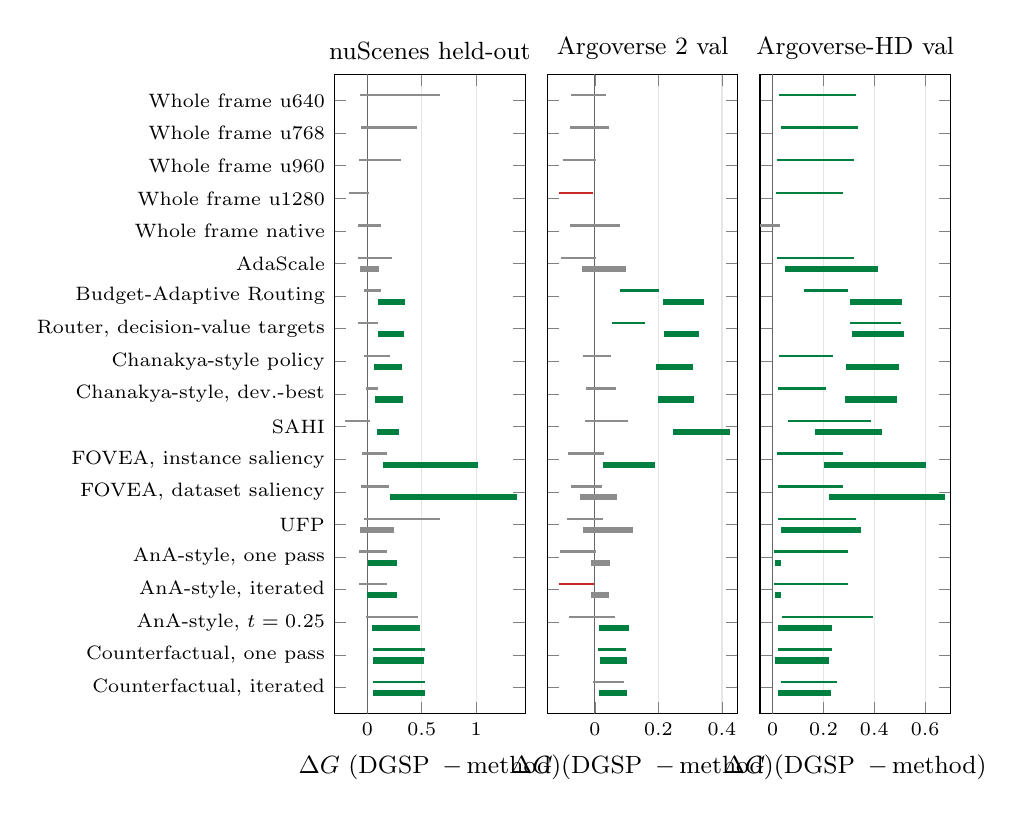
\begin{tikzpicture}
\begin{groupplot}[group style={group size=3 by 1, horizontal sep=8pt, yticklabels at=edge left},
  width=0.33\linewidth, height=0.80\linewidth, scale only axis=false,
  ymin=-0.8, ymax=18.8, ytick={0,...,18}, y dir=reverse,
  yticklabels={{Whole frame u640},{Whole frame u768},{Whole frame u960},{Whole frame u1280},{Whole frame native},{AdaScale},{Budget-Adaptive Routing},{Router, decision-value targets},{Chanakya-style policy},{Chanakya-style, dev.-best},{SAHI},{FOVEA, instance saliency},{FOVEA, dataset saliency},{UFP},{AnA-style, one pass},{AnA-style, iterated},{AnA-style, $t=0.25$},{Counterfactual, one pass},{Counterfactual, iterated}},
  tick label style={font=\scriptsize}, label style={font=\small},
  title style={font=\small, yshift=-4pt}, xmajorgrids, grid style={gray!20},
  xlabel={$\Delta\G$ (\method$\,-\,$method)}]
\nextgroupplot[title={nuScenes held-out}, xmin=-0.30, xmax=1.45]
\draw[black!60] (axis cs:0,-0.8) -- (axis cs:0,18.8);
\draw[black!45, line width=0.9pt] (axis cs:-0.070,-0.17) -- (axis cs:0.666,-0.17);
\draw[black!45, line width=0.9pt] (axis cs:-0.061,0.83) -- (axis cs:0.459,0.83);
\draw[black!45, line width=0.9pt] (axis cs:-0.078,1.83) -- (axis cs:0.308,1.83);
\draw[black!45, line width=0.9pt] (axis cs:-0.165,2.83) -- (axis cs:0.017,2.83);
\draw[black!45, line width=0.9pt] (axis cs:-0.087,3.83) -- (axis cs:0.122,3.83);
\draw[black!45, line width=0.9pt] (axis cs:-0.089,4.83) -- (axis cs:0.228,4.83);
\draw[black!45, line width=2.2pt] (axis cs:-0.065,5.17) -- (axis cs:0.112,5.17);
\draw[black!45, line width=0.9pt] (axis cs:-0.032,5.83) -- (axis cs:0.125,5.83);
\draw[gaingreen, line width=2.2pt] (axis cs:0.096,6.17) -- (axis cs:0.345,6.17);
\draw[black!45, line width=0.9pt] (axis cs:-0.088,6.83) -- (axis cs:0.095,6.83);
\draw[gaingreen, line width=2.2pt] (axis cs:0.094,7.17) -- (axis cs:0.339,7.17);
\draw[black!45, line width=0.9pt] (axis cs:-0.032,7.83) -- (axis cs:0.207,7.83);
\draw[gaingreen, line width=2.2pt] (axis cs:0.064,8.17) -- (axis cs:0.316,8.17);
\draw[black!45, line width=0.9pt] (axis cs:-0.009,8.83) -- (axis cs:0.095,8.83);
\draw[gaingreen, line width=2.2pt] (axis cs:0.071,9.17) -- (axis cs:0.324,9.17);
\draw[black!45, line width=0.9pt] (axis cs:-0.207,9.83) -- (axis cs:0.029,9.83);
\draw[gaingreen, line width=2.2pt] (axis cs:0.090,10.17) -- (axis cs:0.289,10.17);
\draw[black!45, line width=0.9pt] (axis cs:-0.049,10.83) -- (axis cs:0.179,10.83);
\draw[gaingreen, line width=2.2pt] (axis cs:0.148,11.17) -- (axis cs:1.020,11.17);
\draw[black!45, line width=0.9pt] (axis cs:-0.061,11.83) -- (axis cs:0.197,11.83);
\draw[gaingreen, line width=2.2pt] (axis cs:0.206,12.17) -- (axis cs:1.374,12.17);
\draw[black!45, line width=0.9pt] (axis cs:-0.030,12.83) -- (axis cs:0.670,12.83);
\draw[black!45, line width=2.2pt] (axis cs:-0.065,13.17) -- (axis cs:0.243,13.17);
\draw[black!45, line width=0.9pt] (axis cs:-0.074,13.83) -- (axis cs:0.181,13.83);
\draw[gaingreen, line width=2.2pt] (axis cs:0.003,14.17) -- (axis cs:0.273,14.17);
\draw[black!45, line width=0.9pt] (axis cs:-0.074,14.83) -- (axis cs:0.181,14.83);
\draw[gaingreen, line width=2.2pt] (axis cs:0.001,15.17) -- (axis cs:0.270,15.17);
\draw[black!45, line width=0.9pt] (axis cs:-0.014,15.83) -- (axis cs:0.470,15.83);
\draw[gaingreen, line width=2.2pt] (axis cs:0.039,16.17) -- (axis cs:0.485,16.17);
\draw[gaingreen, line width=0.9pt] (axis cs:0.054,16.83) -- (axis cs:0.527,16.83);
\draw[gaingreen, line width=2.2pt] (axis cs:0.049,17.17) -- (axis cs:0.524,17.17);
\draw[gaingreen, line width=0.9pt] (axis cs:0.056,17.83) -- (axis cs:0.530,17.83);
\draw[gaingreen, line width=2.2pt] (axis cs:0.051,18.17) -- (axis cs:0.526,18.17);
\nextgroupplot[title={Argoverse~2 val}, xmin=-0.15, xmax=0.45]
\draw[black!60] (axis cs:0,-0.8) -- (axis cs:0,18.8);
\draw[black!45, line width=0.9pt] (axis cs:-0.076,-0.17) -- (axis cs:0.035,-0.17);
\draw[black!45, line width=0.9pt] (axis cs:-0.080,0.83) -- (axis cs:0.043,0.83);
\draw[black!45, line width=0.9pt] (axis cs:-0.102,1.83) -- (axis cs:0.004,1.83);
\draw[oursc, line width=0.9pt] (axis cs:-0.113,2.83) -- (axis cs:-0.005,2.83);
\draw[black!45, line width=0.9pt] (axis cs:-0.077,3.83) -- (axis cs:0.080,3.83);
\draw[black!45, line width=0.9pt] (axis cs:-0.107,4.83) -- (axis cs:0.002,4.83);
\draw[black!45, line width=2.2pt] (axis cs:-0.040,5.17) -- (axis cs:0.099,5.17);
\draw[gaingreen, line width=0.9pt] (axis cs:0.078,5.83) -- (axis cs:0.201,5.83);
\draw[gaingreen, line width=2.2pt] (axis cs:0.214,6.17) -- (axis cs:0.344,6.17);
\draw[gaingreen, line width=0.9pt] (axis cs:0.053,6.83) -- (axis cs:0.157,6.83);
\draw[gaingreen, line width=2.2pt] (axis cs:0.216,7.17) -- (axis cs:0.328,7.17);
\draw[black!45, line width=0.9pt] (axis cs:-0.039,7.83) -- (axis cs:0.051,7.83);
\draw[gaingreen, line width=2.2pt] (axis cs:0.193,8.17) -- (axis cs:0.309,8.17);
\draw[black!45, line width=0.9pt] (axis cs:-0.028,8.83) -- (axis cs:0.065,8.83);
\draw[gaingreen, line width=2.2pt] (axis cs:0.198,9.17) -- (axis cs:0.311,9.17);
\draw[black!45, line width=0.9pt] (axis cs:-0.031,9.83) -- (axis cs:0.105,9.83);
\draw[gaingreen, line width=2.2pt] (axis cs:0.246,10.17) -- (axis cs:0.424,10.17);
\draw[black!45, line width=0.9pt] (axis cs:-0.086,10.83) -- (axis cs:0.027,10.83);
\draw[gaingreen, line width=2.2pt] (axis cs:0.026,11.17) -- (axis cs:0.189,11.17);
\draw[black!45, line width=0.9pt] (axis cs:-0.074,11.83) -- (axis cs:0.023,11.83);
\draw[black!45, line width=2.2pt] (axis cs:-0.047,12.17) -- (axis cs:0.071,12.17);
\draw[black!45, line width=0.9pt] (axis cs:-0.089,12.83) -- (axis cs:0.026,12.83);
\draw[black!45, line width=2.2pt] (axis cs:-0.038,13.17) -- (axis cs:0.119,13.17);
\draw[black!45, line width=0.9pt] (axis cs:-0.111,13.83) -- (axis cs:0.002,13.83);
\draw[black!45, line width=2.2pt] (axis cs:-0.011,14.17) -- (axis cs:0.047,14.17);
\draw[oursc, line width=0.9pt] (axis cs:-0.113,14.83) -- (axis cs:-0.002,14.83);
\draw[black!45, line width=2.2pt] (axis cs:-0.013,15.17) -- (axis cs:0.045,15.17);
\draw[black!45, line width=0.9pt] (axis cs:-0.081,15.83) -- (axis cs:0.063,15.83);
\draw[gaingreen, line width=2.2pt] (axis cs:0.014,16.17) -- (axis cs:0.107,16.17);
\draw[gaingreen, line width=0.9pt] (axis cs:0.011,16.83) -- (axis cs:0.098,16.83);
\draw[gaingreen, line width=2.2pt] (axis cs:0.016,17.17) -- (axis cs:0.101,17.17);
\draw[black!45, line width=0.9pt] (axis cs:-0.005,17.83) -- (axis cs:0.090,17.83);
\draw[gaingreen, line width=2.2pt] (axis cs:0.014,18.17) -- (axis cs:0.102,18.17);
\nextgroupplot[title={Argoverse-HD val}, xmin=-0.05, xmax=0.70]
\draw[black!60] (axis cs:0,-0.8) -- (axis cs:0,18.8);
\draw[gaingreen, line width=0.9pt] (axis cs:0.026,-0.17) -- (axis cs:0.329,-0.17);
\draw[gaingreen, line width=0.9pt] (axis cs:0.032,0.83) -- (axis cs:0.336,0.83);
\draw[gaingreen, line width=0.9pt] (axis cs:0.017,1.83) -- (axis cs:0.320,1.83);
\draw[gaingreen, line width=0.9pt] (axis cs:0.013,2.83) -- (axis cs:0.278,2.83);
\draw[black!45, line width=0.9pt] (axis cs:-0.048,3.83) -- (axis cs:0.028,3.83);
\draw[gaingreen, line width=0.9pt] (axis cs:0.017,4.83) -- (axis cs:0.319,4.83);
\draw[gaingreen, line width=2.2pt] (axis cs:0.050,5.17) -- (axis cs:0.414,5.17);
\draw[gaingreen, line width=0.9pt] (axis cs:0.124,5.83) -- (axis cs:0.297,5.83);
\draw[gaingreen, line width=2.2pt] (axis cs:0.304,6.17) -- (axis cs:0.508,6.17);
\draw[gaingreen, line width=0.9pt] (axis cs:0.306,6.83) -- (axis cs:0.505,6.83);
\draw[gaingreen, line width=2.2pt] (axis cs:0.313,7.17) -- (axis cs:0.516,7.17);
\draw[gaingreen, line width=0.9pt] (axis cs:0.025,7.83) -- (axis cs:0.237,7.83);
\draw[gaingreen, line width=2.2pt] (axis cs:0.290,8.17) -- (axis cs:0.497,8.17);
\draw[gaingreen, line width=0.9pt] (axis cs:0.020,8.83) -- (axis cs:0.209,8.83);
\draw[gaingreen, line width=2.2pt] (axis cs:0.285,9.17) -- (axis cs:0.490,9.17);
\draw[gaingreen, line width=0.9pt] (axis cs:0.062,9.83) -- (axis cs:0.388,9.83);
\draw[gaingreen, line width=2.2pt] (axis cs:0.166,10.17) -- (axis cs:0.430,10.17);
\draw[gaingreen, line width=0.9pt] (axis cs:0.016,10.83) -- (axis cs:0.278,10.83);
\draw[gaingreen, line width=2.2pt] (axis cs:0.202,11.17) -- (axis cs:0.602,11.17);
\draw[gaingreen, line width=0.9pt] (axis cs:0.019,11.83) -- (axis cs:0.276,11.83);
\draw[gaingreen, line width=2.2pt] (axis cs:0.222,12.17) -- (axis cs:0.677,12.17);
\draw[gaingreen, line width=0.9pt] (axis cs:0.021,12.83) -- (axis cs:0.328,12.83);
\draw[gaingreen, line width=2.2pt] (axis cs:0.032,13.17) -- (axis cs:0.346,13.17);
\draw[gaingreen, line width=0.9pt] (axis cs:0.007,13.83) -- (axis cs:0.297,13.83);
\draw[gaingreen, line width=2.2pt] (axis cs:0.008,14.17) -- (axis cs:0.034,14.17);
\draw[gaingreen, line width=0.9pt] (axis cs:0.006,14.83) -- (axis cs:0.296,14.83);
\draw[gaingreen, line width=2.2pt] (axis cs:0.008,15.17) -- (axis cs:0.034,15.17);
\draw[gaingreen, line width=0.9pt] (axis cs:0.036,15.83) -- (axis cs:0.396,15.83);
\draw[gaingreen, line width=2.2pt] (axis cs:0.020,16.17) -- (axis cs:0.232,16.17);
\draw[gaingreen, line width=0.9pt] (axis cs:0.019,16.83) -- (axis cs:0.233,16.83);
\draw[gaingreen, line width=2.2pt] (axis cs:0.008,17.17) -- (axis cs:0.222,17.17);
\draw[gaingreen, line width=0.9pt] (axis cs:0.033,17.83) -- (axis cs:0.253,17.83);
\draw[gaingreen, line width=2.2pt] (axis cs:0.020,18.17) -- (axis cs:0.228,18.17);
\end{groupplot}
\end{tikzpicture}
\caption{\textbf{Is any compared method significantly better than \method?} $95\%$ paired intervals of \method$\,-\,$method without a cap (thin) and under the per-frame cap at the pixels of \method (thick). Green: \method significantly better; red: significantly worse; grey: not significant. Under the cap, no interval lies below zero. Whole-frame rows have no cap. Values in \cref{tab:main_ci}.}
\label{fig:forest}
\end{figure}

Under the per-frame cap, \method is significantly better in $35$ of the $42$ comparisons with these $14$ methods and variants ($29$ of the $36$ with the $12$ primary methods), and no method is significantly better.
The strongest object-level alternative on Argoverse~2, iterated AnA-style refinement, finds the decisive object as often as \method ($96.1\%$ \vs $96.5\%$ of the frames that require braking) and, where both find it, with the same estimated range; it verifies every corridor detection on every frame with $1.5\times$ the pixels of \method, which gives the learned looming estimate a continuous history, and under the cap, it falls below \method.
\method produces $4.2$, $5.6$, and $15.0$ spurious braking detections per $1{,}000$ frames on the three datasets, the fewest of all methods with a positive decision value on nuScenes.

\subsection{Whole-frame inference with and without the components}
\label{sec:supp_uniform}

\begin{figure}[!htbp]
\centering
% plot generated from the reference tables (script: versions/paper_tools_2026-10-27/make_supp_figs.py)
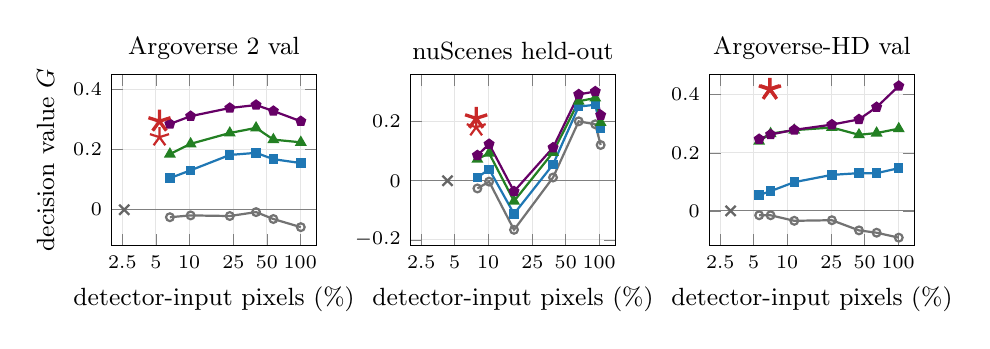
\begin{tikzpicture}
\begin{groupplot}[group style={group size=3 by 1, horizontal sep=34pt},
  width=0.345\linewidth, height=0.31\linewidth, xmode=log, xmin=0.02, xmax=1.4,
  xtick={0.025,0.05,0.1,0.25,0.5,1.0}, xticklabels={2.5,5,10,25,50,100},
  yticklabel style={/pgf/number format/fixed, /pgf/number format/precision=1},
  xlabel={detector-input pixels (\%)}, tick label style={font=\scriptsize}, label style={font=\small},
  title style={font=\small, yshift=-4pt}, grid=major, grid style={gray!20},
  legend style={font=\scriptsize, draw=gray!50, column sep=4pt}, legend cell align=left]
\nextgroupplot[title={Argoverse~2 val}, ymin=-0.12, ymax=0.45, ylabel={decision value $\G$}, legend to name=unilegend, legend columns=3]
\draw[black!50, thin] (axis cs:0.02,0) -- (axis cs:1.4,0);
\addplot[black!55, thick, mark=o, mark size=1.4pt] coordinates {(0.067,-0.025) (0.103,-0.019) (0.232,-0.021) (0.400,-0.008) (0.573,-0.031) (1.012,-0.058)};
\addlegendentry{Plain}
\addplot[adac, thick, mark=square*, mark size=1.3pt] coordinates {(0.067,0.105) (0.103,0.131) (0.232,0.182) (0.400,0.189) (0.573,0.168) (1.012,0.155)};
\addlegendentry{+ refiner}
\addplot[cropc!80!black, thick, mark=triangle*, mark size=1.7pt] coordinates {(0.067,0.185) (0.103,0.219) (0.232,0.255) (0.400,0.272) (0.573,0.233) (1.012,0.224)};
\addlegendentry{+ refiner + hand-crafted looming}
\addplot[violet!80!black, thick, mark=pentagon*, mark size=1.6pt] coordinates {(0.067,0.285) (0.103,0.311) (0.232,0.338) (0.400,0.348) (0.573,0.328) (1.012,0.294)};
\addlegendentry{+ refiner + learned looming}
\addplot[black!60, only marks, mark=x, mark size=2.6pt, thick] coordinates {(0.026,0)};
\addlegendentry{cheap detector (u320)}
\addplot[oursc, only marks, mark=star, mark size=3.6pt, thick, mark options={fill=white}] coordinates {(0.054,0.241)};
\addlegendentry{\method w/o refiner}
\addplot[oursc, only marks, mark=star, mark size=4.2pt, very thick] coordinates {(0.054,0.294)};
\addlegendentry{\method}
\nextgroupplot[title={nuScenes held-out}, ymin=-0.22, ymax=0.36]
\draw[black!50, thin] (axis cs:0.02,0) -- (axis cs:1.4,0);
\addplot[black!55, thick, mark=o, mark size=1.4pt] coordinates {(0.080,-0.026) (0.102,-0.003) (0.171,-0.166) (0.384,0.011) (0.654,0.201) (0.922,0.191) (1.031,0.121)};
\addplot[adac, thick, mark=square*, mark size=1.3pt] coordinates {(0.080,0.011) (0.102,0.039) (0.171,-0.112) (0.384,0.055) (0.654,0.251) (0.922,0.257) (1.031,0.176)};
\addplot[cropc!80!black, thick, mark=triangle*, mark size=1.7pt] coordinates {(0.080,0.073) (0.102,0.093) (0.171,-0.069) (0.384,0.096) (0.654,0.269) (0.922,0.280) (1.031,0.197)};
\addplot[violet!80!black, thick, mark=pentagon*, mark size=1.6pt] coordinates {(0.080,0.086) (0.102,0.124) (0.171,-0.036) (0.384,0.112) (0.654,0.292) (0.922,0.302) (1.031,0.222)};
\addplot[black!60, only marks, mark=x, mark size=2.6pt, thick] coordinates {(0.043,0)};
\addplot[oursc, only marks, mark=star, mark size=3.6pt, thick, mark options={fill=white}] coordinates {(0.078,0.181)};
\addplot[oursc, only marks, mark=star, mark size=4.2pt, very thick] coordinates {(0.078,0.211)};
\nextgroupplot[title={Argoverse-HD val}, ymin=-0.12, ymax=0.47]
\draw[black!50, thin] (axis cs:0.02,0) -- (axis cs:1.4,0);
\addplot[black!55, thick, mark=o, mark size=1.4pt] coordinates {(0.056,-0.015) (0.071,-0.015) (0.116,-0.034) (0.253,-0.032) (0.444,-0.067) (0.640,-0.075) (1.013,-0.092)};
\addplot[adac, thick, mark=square*, mark size=1.3pt] coordinates {(0.056,0.055) (0.071,0.068) (0.116,0.099) (0.253,0.124) (0.444,0.130) (0.640,0.130) (1.013,0.147)};
\addplot[cropc!80!black, thick, mark=triangle*, mark size=1.7pt] coordinates {(0.056,0.240) (0.071,0.266) (0.116,0.278) (0.253,0.287) (0.444,0.262) (0.640,0.268) (1.013,0.283)};
\addplot[violet!80!black, thick, mark=pentagon*, mark size=1.6pt] coordinates {(0.056,0.247) (0.071,0.263) (0.116,0.279) (0.253,0.297) (0.444,0.315) (0.640,0.357) (1.013,0.430)};
\addplot[black!60, only marks, mark=x, mark size=2.6pt, thick] coordinates {(0.031,0)};
\addplot[oursc, only marks, mark=star, mark size=3.6pt, thick, mark options={fill=white}] coordinates {(0.070,0.422)};
\addplot[oursc, only marks, mark=star, mark size=4.2pt, very thick] coordinates {(0.070,0.418)};
\end{groupplot}
\end{tikzpicture}

\vspace{2pt}
\pgfplotslegendfromname{unilegend}
\caption{\textbf{How much of the gain is due to the components?} Decision value of whole-frame inference at each long side, without and with the shared components, \vs detector-input pixels (log scale). The components raise the decision value at every resolution. \method lies above the curve with the refiner on Argoverse~2 and Argoverse-HD, and whole-frame inference with both components exceeds it only with $1.9\times$, $8.4\times$, and $14.5\times$ its pixels on Argoverse~2, nuScenes, and Argoverse-HD. Values in \cref{tab:uniform}; intervals in \cref{tab:uniform_ci}.}
\label{fig:uniform}
\end{figure}

% --- Fig.: decision value vs. network pixels (handoff/K28 phase2/table_main_{av2,nusc,ahd}_v6.csv: plain whole frame; dashed = C1 column of tab:uniform, i.e. + refiner + learned looming; DESP = v6-S) ---
\begin{figure}[!htbp]
\centering
\begin{minipage}{0.52\linewidth}\centering
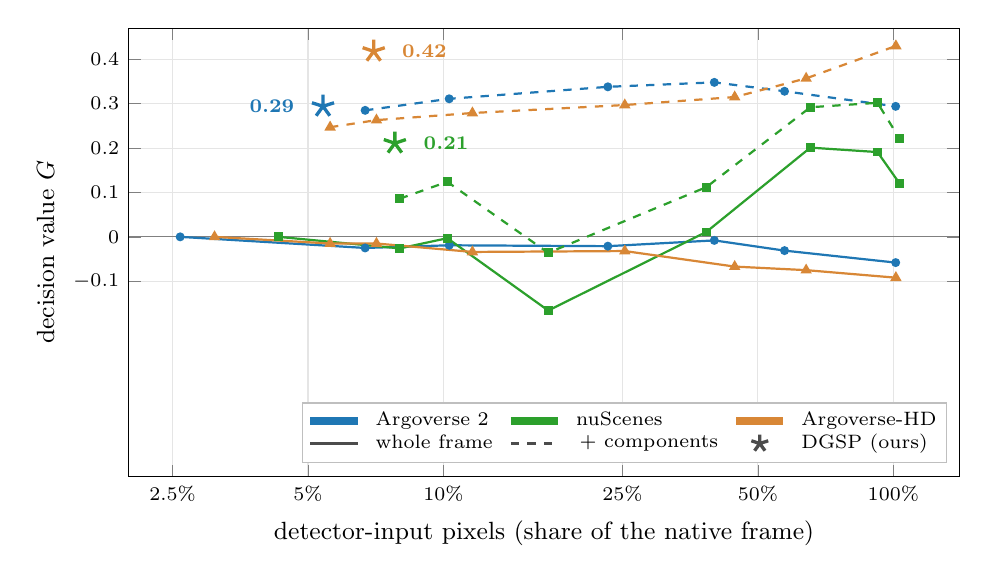
\begin{tikzpicture}
\begin{axis}[
  width=\linewidth, height=0.60\linewidth,
  xmode=log, xmin=0.02, xmax=1.4, ymin=-0.54, ymax=0.47,
  ytick={-0.1,0,0.1,0.2,0.3,0.4},
  yticklabel style={/pgf/number format/fixed, /pgf/number format/precision=1},
  xtick={0.025,0.05,0.1,0.25,0.5,1.0},
  xticklabels={2.5\%,5\%,10\%,25\%,50\%,100\%},
  xlabel={detector-input pixels (share of the native frame)},
  ylabel={decision value $\G$},
  tick label style={font=\scriptsize}, label style={font=\small},
  grid=major, grid style={gray!20},
  legend style={font=\scriptsize, at={(0.985,0.03)}, anchor=south east, draw=gray!50, row sep=-2.5pt, inner sep=1.5pt, column sep=3pt},
  legend columns=3, legend cell align=left,
]
\draw[black!50, thin] (axis cs:0.02,0) -- (axis cs:1.4,0);
% whole frame at increasing resolution (first point: cheap detector, G = 0); solid: plain, dashed: + refiner + C1
\addplot[adac, thick, mark=*, mark size=1.2pt, forget plot] coordinates
{(0.026,0) (0.067,-0.025) (0.103,-0.019) (0.232,-0.021) (0.400,-0.008) (0.573,-0.031) (1.012,-0.058)};
\addplot[cropc, thick, mark=square*, mark size=1.2pt, forget plot] coordinates
{(0.043,0) (0.080,-0.026) (0.102,-0.003) (0.171,-0.166) (0.384,0.011) (0.654,0.201) (0.922,0.191) (1.031,0.121)};
\addplot[fieldc!90!black, thick, mark=triangle*, mark size=1.6pt, forget plot] coordinates
{(0.031,0) (0.056,-0.015) (0.071,-0.015) (0.116,-0.034) (0.253,-0.032) (0.444,-0.067) (0.640,-0.075) (1.013,-0.092)};
\addplot[adac, thick, dashed, mark=*, mark size=1.2pt, mark options={solid}, forget plot] coordinates
{(0.067,0.285) (0.103,0.311) (0.232,0.338) (0.400,0.348) (0.573,0.328) (1.012,0.294)};
\addplot[cropc, thick, dashed, mark=square*, mark size=1.2pt, mark options={solid}, forget plot] coordinates
{(0.080,0.086) (0.102,0.124) (0.171,-0.036) (0.384,0.112) (0.654,0.292) (0.922,0.302) (1.031,0.222)};
\addplot[fieldc!90!black, thick, dashed, mark=triangle*, mark size=1.6pt, mark options={solid}, forget plot] coordinates
{(0.056,0.247) (0.071,0.263) (0.116,0.279) (0.253,0.297) (0.444,0.315) (0.640,0.357) (1.013,0.430)};
\addlegendimage{adac, line width=3pt}
\addlegendentry{Argoverse~2}
\addlegendimage{cropc, line width=3pt}
\addlegendentry{nuScenes}
\addlegendimage{fieldc!90!black, line width=3pt}
\addlegendentry{Argoverse-HD}
\addlegendimage{black!70, thick}
\addlegendentry{whole frame}
\addlegendimage{black!70, thick, dashed}
\addlegendentry{\,+ components}
\addlegendimage{black!70, only marks, mark=star, mark size=3.2pt, very thick}
\addlegendentry{\method (ours)}
% ours
\addplot[adac, only marks, mark=star, mark size=4.2pt, very thick, forget plot] coordinates {(0.054,0.294)};
\addplot[cropc, only marks, mark=star, mark size=4.2pt, very thick, forget plot] coordinates {(0.078,0.211)};
\addplot[fieldc!90!black, only marks, mark=star, mark size=4.2pt, very thick, forget plot] coordinates {(0.070,0.418)};
\node[font=\scriptsize\bfseries, text=adac, anchor=east] at (axis cs:0.049,0.294) {0.29};
\node[font=\scriptsize\bfseries, text=cropc, anchor=west] at (axis cs:0.086,0.211) {0.21};
\node[font=\scriptsize\bfseries, text=fieldc!90!black, anchor=west] at (axis cs:0.077,0.418) {0.42};
\end{axis}
\end{tikzpicture}
\end{minipage}
\caption{\textbf{Decision value \vs detector-input pixels.} Whole-frame YOLOv8s from a long side of $320$ pixels (the cheap pipeline, $\G=0$) to the native resolution, without (solid) and with (dashed) the shared components; stars: \method.}
\label{fig:gpx}
\end{figure}

\Cref{fig:gpx} plots the decision value of whole-frame inference against its pixels, and \cref{tab:uniform} lists the plotted values, together with whole-frame inference that is equipped with the shared components, and \cref{tab:uniform_ci} the intervals with the refiner in both pipelines.
\method is significantly better than whole-frame inference with the refiner at every resolution on Argoverse~2 and Argoverse-HD and at the three lowest resolutions on nuScenes.
With the learned looming estimate in addition, \method remains significantly better at every long side up to $1280$ pixels on Argoverse-HD, with lower interval bounds between $0.013$ and $0.028$.

\subsection{Crop heuristics under nominal and strict pixel caps}
\label{sec:supp_heuristics}

\begin{table}[!htbp]
\centering
\caption{\textbf{Crop heuristics with identical components at matched budgets.} No heuristic is significantly better than \method in either setting. Left: smallest budget of the tuned grid of each heuristic; ``Single'': with the refiner and the looming cue of a single pair of boxes; ``Learned'': with the refiner and the learned looming estimate; $\Delta$ against the heuristic with the learned estimate. Right: capped at the pixels of \method on every frame, with the learned estimate; ``px'': realized detector-input pixels relative to \method (the truncation guard lets the heuristics exceed the cap). Bold intervals: above zero.}
\label{tab:heuristics}
\small
\setlength{\tabcolsep}{4pt}
\begin{tabular}{@{}lcccccccc@{}}
\toprule
 & \multicolumn{4}{c}{Smallest budget of the tuned grid} & & \multicolumn{3}{c}{Per-frame cap at the pixels of \method} \\
\cmidrule(lr){2-5}\cmidrule(l){7-9}
Heuristic & px\,(\%) & $\G$, single & $\G$, learned & $\Delta$ & & $\G$ & px & $\Delta$ \\
\midrule
\multicolumn{9}{@{}l}{\emph{nuScenes held-out}} \\
Uncertainty & 10.2 & $-$0.067 & $-$0.059 & \best{\ci{+0.032}{+0.483}} &  & $-$0.058 & $1.32\times$ & \best{\ci{+0.030}{+0.481}} \\
Temporal criticality & 9.4 & 0.142 & 0.173 & \best{\ci{+0.008}{+0.076}} &  & 0.167 & $1.22\times$ & \best{\ci{+0.014}{+0.082}} \\
Ego corridor & 10.1 & 0.026 & 0.052 & \best{\ci{+0.021}{+0.314}} &  & 0.053 & $1.30\times$ & \best{\ci{+0.020}{+0.312}} \\
Support + ego corridor & 10.8 & 0.148 & 0.174 & \ci{-0.012}{+0.096} &  & 0.174 & $1.40\times$ & \ci{-0.012}{+0.096} \\
Random & 12.2 & $-$0.034 & $-$0.037 & \best{\ci{+0.100}{+0.420}} &  & \na & \na & \na \\
\oursrow \textbf{\method} & 7.8 & \multicolumn{2}{c}{\textbf{0.211}} & \na &  & \textbf{0.211} & $1.00\times$ & \na \\
\midrule
\multicolumn{9}{@{}l}{\emph{Argoverse~2 val}} \\
Uncertainty & 8.0 & 0.163 & 0.219 & \best{\ci{+0.020}{+0.126}} &  & 0.221 & $1.51\times$ & \best{\ci{+0.018}{+0.123}} \\
Temporal criticality & 8.3 & 0.157 & 0.242 & \best{\ci{+0.006}{+0.093}} &  & 0.246 & $1.55\times$ & \best{\ci{+0.002}{+0.090}} \\
Ego corridor & 6.6 & 0.174 & 0.260 & \best{\ci{+0.011}{+0.062}} &  & 0.262 & $1.24\times$ & \best{\ci{+0.010}{+0.060}} \\
Support + ego corridor & 7.1 & 0.194 & 0.296 & \ci{-0.013}{+0.007} &  & 0.296 & $1.33\times$ & \ci{-0.014}{+0.008} \\
Random & 8.9 & 0.061 & 0.018 & \best{\ci{+0.212}{+0.347}} &  & \na & \na & \na \\
\oursrow \textbf{\method} & 5.4 & \multicolumn{2}{c}{\textbf{0.294}} & \na &  & 0.294 & $1.00\times$ & \na \\
\midrule
\multicolumn{9}{@{}l}{\emph{Argoverse-HD val}} \\
Uncertainty & 12.3 & 0.141 & 0.282 & \best{\ci{+0.049}{+0.252}} &  & 0.285 & $1.76\times$ & \best{\ci{+0.046}{+0.249}} \\
Temporal criticality & 11.6 & 0.185 & 0.378 & \best{\ci{+0.007}{+0.079}} &  & 0.377 & $1.66\times$ & \best{\ci{+0.009}{+0.080}} \\
Ego corridor & 10.9 & 0.183 & 0.389 & \best{\ci{+0.001}{+0.063}} &  & 0.393 & $1.55\times$ & \ci{-0.004}{+0.062} \\
Support + ego corridor & 10.8 & 0.180 & 0.408 & \ci{-0.001}{+0.023} &  & 0.409 & $1.54\times$ & \ci{-0.002}{+0.022} \\
Random & 16.6 & 0.039 & 0.139 & \best{\ci{+0.192}{+0.362}} &  & \na & \na & \na \\
\oursrow \textbf{\method} & 7.0 & \multicolumn{2}{c}{\textbf{0.418}} & \na &  & \textbf{0.418} & $1.00\times$ & \na \\
\bottomrule
\end{tabular}
\end{table}

At the smallest budget of their tuned grid, the heuristics receive $1.2$ to $2.4\times$ the detector-input pixels of \method; \method significantly outperforms four of the five on all three datasets and matches the heuristic that combines its own support with an ego-corridor tube.
The learned looming estimate raises the decision value of every informed heuristic on all three datasets, and \method retains its advantage when the heuristics are given it; the advantage therefore stems from the selection of the regions.

In \cref{tab:heuristics}, every heuristic is capped at the pixels of \method on the same frame.
\method significantly outperforms the uncertainty and temporal-criticality heuristics on all three datasets and the ego-corridor heuristic on nuScenes and Argoverse~2, and it matches the remaining ones, although the guard lets the heuristics exceed the cap by $22$--$76\%$.

% --- Table: strict post-guard cap (handoff/K39/k39_2_rows.csv, k39_2_diffs.csv) ---
\begin{table}[!htbp]
\centering
\caption{\textbf{Strict per-frame cap including the truncation guard.} Each crop or guard re-detection that would raise the detector-input pixels of a frame above those of \method on that frame is skipped, and a pending truncated detection is then kept as detected; the realized pixels never exceed those of \method. All rows use the refiner and the learned looming estimate. The primary variant of each heuristic was fixed by a rule on the development data before the run; $\Delta$: \method minus the row; px: realized pixels in \% of the native frame.}
\label{tab:strictcap}
\small
\setlength{\tabcolsep}{3pt}
\begin{tabular}{@{}lcccccccc@{}}
\toprule
 & \multicolumn{2}{c}{nuScenes held-out} & & \multicolumn{2}{c}{Argoverse~2 val} & & \multicolumn{2}{c}{Argoverse-HD val} \\
\cmidrule(lr){2-3}\cmidrule(lr){5-6}\cmidrule(l){8-9}
Primary row & $\G$ (px) & $\Delta$ & & $\G$ (px) & $\Delta$ & & $\G$ (px) & $\Delta$ \\
\midrule
Support + ego corridor (hybrid) & 0.179 (7.5) & \best{\ci{+0.012}{+0.051}} & & 0.274 (5.1) & \best{\ci{+0.010}{+0.031}} & & 0.392 (6.8) & \best{\ci{+0.011}{+0.046}} \\
Uncertainty & $-$0.060 (6.5) & \best{\ci{+0.058}{+0.435}} & & 0.016 (4.8) & \best{\ci{+0.186}{+0.370}} & & 0.280 (6.3) & \best{\ci{+0.017}{+0.263}} \\
Temporal criticality & 0.153 (6.6) & \best{\ci{+0.022}{+0.105}} & & 0.207 (5.0) & \best{\ci{+0.052}{+0.127}} & & 0.383 (6.7) & \best{\ci{+0.004}{+0.073}} \\
Ego corridor & 0.077 (7.5) & \best{\ci{+0.033}{+0.233}} & & 0.114 (4.8) & \best{\ci{+0.103}{+0.265}} & & 0.377 (6.5) & \ci{-0.006}{+0.099} \\
\midrule
\oursrow \textbf{\method} & \textbf{0.211} (7.8) & \na & & \textbf{0.294} (5.4) & \na & & \textbf{0.418} (7.0) & \na \\
\bottomrule
\end{tabular}
\end{table}

\noindent\textbf{Strict cap.}
Under the nominal cap, the guard lets the hybrid and the heuristics use $1.10$--$1.47\times$ the pixels of \method on average and up to $5$--$13\times$ on single frames.
Under the strict cap of \cref{tab:strictcap}, which includes the guard, \method is significantly better than the hybrid on all three datasets, which it only matches under the nominal cap, and than the primary uncertainty, temporal-criticality, and ego-corridor heuristics in $8$ of $9$ comparisons; the exception is the ego corridor on Argoverse-HD ($+0.041$, $\ci{-0.006}{+0.099}$).
Against the secondary variant of each heuristic, \method is significantly better in $7$ of $9$ comparisons; on Argoverse-HD, it does not differ significantly from the other temporal-criticality variant ($+0.034$) and from the other ego-corridor variant, whose point estimate is higher ($0.458$, $\Delta=-0.040$, $\ci{-0.144}{+0.061}$). Against the other hybrid variant, it is significantly better on nuScenes and Argoverse-HD and not on Argoverse~2 ($+0.013$, $\ci{-0.003}{+0.029}$).
With an equal pixel budget that includes the guard, the selection of the regions therefore matters, and the ties of the hybrid under the nominal cap stem from its additional guard pixels.

On the Jetson (\cref{tab:latency}, same frames), the capped hybrid attains the decision value of \method ($0.373$ \vs $0.380$ on nuScenes and $0.417$ \vs $0.419$ on Argoverse~2) at a higher mean and $95$th-percentile latency ($24.0$ and $75.0$\,ms \vs $21.5$ and $57.7$\,ms; $44.5$ and $109.0$\,ms \vs $39.9$ and $89.5$\,ms).
Along the pixel axis of \method, the decision value is insensitive to the crop parameters: crops with a long side of up to $1280$ pixels and a support context of up to three box sizes change $\G$ by $-0.037$ to $+0.020$ on nuScenes and add at most $0.017$ on Argoverse~2 and Argoverse-HD at $1.4$--$1.8\times$ the pixels.

% --- Fig.: budget sweep with identical components (handoff/K28 phase2/table_main_*_v6.csv, best tuned variant per budget, + C1) ---
\begin{figure}[!tbp]
\centering
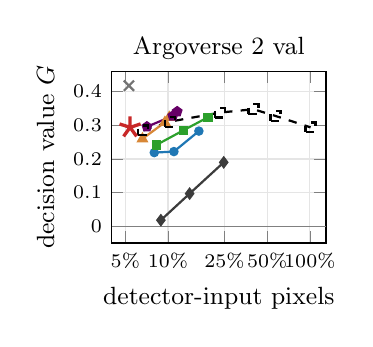
\begin{tikzpicture}
\begin{axis}[
    width=0.355\textwidth, height=0.31\textwidth,
    xmode=log, xmin=0.04, xmax=1.3, ymin=-0.05, ymax=0.46,
    xtick={0.05,0.1,0.25,0.5,1.0}, xticklabels={5\%,10\%,25\%,50\%,100\%},
    ytick={0,0.1,0.2,0.3,0.4},
    yticklabel style={/pgf/number format/fixed, /pgf/number format/precision=1},
    xlabel={detector-input pixels}, ylabel={decision value $\G$},
    title={Argoverse~2 val}, title style={font=\small, yshift=-5pt},
    tick label style={font=\scriptsize}, label style={font=\small},
    grid=major, grid style={gray!20},
    legend to name=paretolegend, legend columns=4,
    legend style={font=\scriptsize, draw=gray!50, column sep=5pt}, legend cell align=left,
]
\draw[black!50, thin] (axis cs:0.04,0) -- (axis cs:1.3,0);
\addplot[adac, thick, mark=*, mark size=1.3pt] coordinates {(0.080,0.219) (0.110,0.222) (0.165,0.283)};
\addlegendentry{Uncertainty crops}
\addplot[cropc, thick, mark=square*, mark size=1.3pt] coordinates {(0.083,0.242) (0.128,0.285) (0.191,0.324)};
\addlegendentry{Temporal-criticality crops}
\addplot[fieldc!90!black, thick, mark=triangle*, mark size=1.7pt] coordinates {(0.066,0.260) (0.095,0.309) (0.102,0.324)};
\addlegendentry{Ego-corridor crops}
\addplot[violet!80!black, thick, mark=pentagon*, mark size=1.6pt] coordinates {(0.071,0.296) (0.108,0.328) (0.116,0.341)};
\addlegendentry{Support + ego-corridor crops}
\addplot[unic, thick, mark=diamond*, mark size=1.7pt] coordinates {(0.089,0.018) (0.142,0.097) (0.247,0.190)};
\addlegendentry{Random crops}
\addplot[black, thick, dashed, mark=square, mark size=1.8pt] coordinates {(0.067,0.285) (0.103,0.311) (0.232,0.338) (0.400,0.348) (0.573,0.328) (1.012,0.294)};
\addlegendentry{Whole frame}
\addplot[black!55, only marks, mark=x, mark size=2.6pt, thick] coordinates {(0.053,0.418)};
\addlegendentry{Oracle router}
\addplot[oursc, only marks, mark=star, mark size=4pt, very thick] coordinates {(0.054,0.294)};
\addlegendentry{\method}
\end{axis}
\end{tikzpicture}\hfill
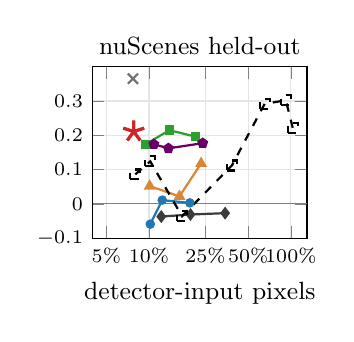
\begin{tikzpicture}
\begin{axis}[
    width=0.355\textwidth, height=0.31\textwidth,
    xmode=log, xmin=0.04, xmax=1.3, ymin=-0.10, ymax=0.40,
    xtick={0.05,0.1,0.25,0.5,1.0}, xticklabels={5\%,10\%,25\%,50\%,100\%},
    ytick={-0.1,0,0.1,0.2,0.3},
    yticklabel style={/pgf/number format/fixed, /pgf/number format/precision=1},
    xlabel={detector-input pixels},
    title={nuScenes held-out}, title style={font=\small, yshift=-5pt},
    tick label style={font=\scriptsize}, label style={font=\small},
    grid=major, grid style={gray!20},
]
\draw[black!50, thin] (axis cs:0.04,0) -- (axis cs:1.3,0);
\addplot[adac, thick, mark=*, mark size=1.3pt] coordinates {(0.102,-0.059) (0.124,0.011) (0.194,0.003)};
\addplot[cropc, thick, mark=square*, mark size=1.3pt] coordinates {(0.094,0.173) (0.139,0.215) (0.213,0.196)};
\addplot[fieldc!90!black, thick, mark=triangle*, mark size=1.7pt] coordinates {(0.101,0.052) (0.164,0.022) (0.233,0.118)};
\addplot[violet!80!black, thick, mark=pentagon*, mark size=1.6pt] coordinates {(0.108,0.174) (0.137,0.162) (0.239,0.177)};
\addplot[unic, thick, mark=diamond*, mark size=1.7pt] coordinates {(0.122,-0.037) (0.196,-0.031) (0.344,-0.027)};
\addplot[black, thick, dashed, mark=square, mark size=1.8pt] coordinates {(0.080,0.086) (0.102,0.124) (0.171,-0.036) (0.384,0.112) (0.654,0.292) (0.922,0.302) (1.031,0.222)};
\addplot[black!55, only marks, mark=x, mark size=2.6pt, thick] coordinates {(0.077,0.365)};
\addplot[oursc, only marks, mark=star, mark size=4pt, very thick] coordinates {(0.078,0.211)};
\end{axis}
\end{tikzpicture}\hfill
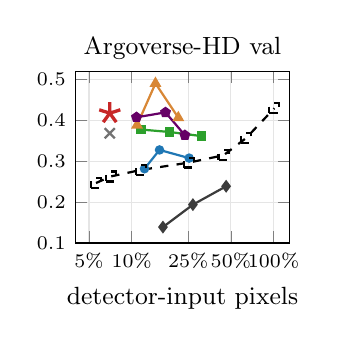
\begin{tikzpicture}
\begin{axis}[
    width=0.355\textwidth, height=0.31\textwidth,
    xmode=log, xmin=0.04, xmax=1.3, ymin=0.10, ymax=0.52,
    xtick={0.05,0.1,0.25,0.5,1.0}, xticklabels={5\%,10\%,25\%,50\%,100\%},
    ytick={0.1,0.2,0.3,0.4,0.5},
    yticklabel style={/pgf/number format/fixed, /pgf/number format/precision=1},
    xlabel={detector-input pixels},
    title={Argoverse-HD val}, title style={font=\small, yshift=-5pt},
    tick label style={font=\scriptsize}, label style={font=\small},
    grid=major, grid style={gray!20},
]
\addplot[adac, thick, mark=*, mark size=1.3pt] coordinates {(0.123,0.282) (0.157,0.328) (0.254,0.308)};
\addplot[cropc, thick, mark=square*, mark size=1.3pt] coordinates {(0.116,0.378) (0.185,0.372) (0.309,0.362)};
\addplot[fieldc!90!black, thick, mark=triangle*, mark size=1.7pt] coordinates {(0.109,0.389) (0.147,0.491) (0.213,0.407)};
\addplot[violet!80!black, thick, mark=pentagon*, mark size=1.6pt] coordinates {(0.108,0.408) (0.173,0.420) (0.237,0.364)};
\addplot[unic, thick, mark=diamond*, mark size=1.7pt] coordinates {(0.166,0.139) (0.270,0.194) (0.463,0.239)};
\addplot[black, thick, dashed, mark=square, mark size=1.8pt] coordinates {(0.056,0.247) (0.071,0.263) (0.116,0.279) (0.253,0.297) (0.444,0.315) (0.640,0.357) (1.013,0.430)};
\addplot[black!55, only marks, mark=x, mark size=2.6pt, thick] coordinates {(0.070,0.369)};
\addplot[oursc, only marks, mark=star, mark size=4pt, very thick] coordinates {(0.070,0.418)};
\end{axis}
\end{tikzpicture}

\vspace{2pt}
\pgfplotslegendfromname{paretolegend}
\caption{\textbf{Decision value \vs detector-input pixels with identical components.} All baselines use the range refiner and the learned looming estimate of \method, and the crop heuristics also its truncation guard and scene history; each heuristic is shown with its best tuned variant at three budgets. The oracle router escalates the frames with the highest true decision value and is not realizable.}
\label{fig:pareto}
\end{figure}

\subsection{Mean pixel budget for the frame-level methods}
\label{sec:supp_meanbudget}

% --- K40-3 / D01 (handoff/K40R/k40_3_mean_budget.csv, k40_3_family_summary.csv; pre-specified post-hoc, own routed history) ---
\begin{table}[!htbp]
\centering
\caption{\textbf{Frame-level methods under a mean pixel budget} instead of the per-frame cap of \mref{tab:main}, each run with its own routed history and the refiner. Thresholds are set on the development data of nuScenes and Argoverse~2 to meet the mean pixels of \method; Argoverse-HD uses those of Argoverse~2. px: realized mean pixels relative to \method on the test split; AdaScale cannot meet the budget with its scale ladder and uses its closest policy. $\Delta$: \method minus the row.}
\label{tab:meanbudget}
\footnotesize
\setlength{\tabcolsep}{2.2pt}
\begin{tabular}{@{}lcccccccc@{}}
\toprule
 & \multicolumn{2}{c}{nuScenes held-out} & & \multicolumn{2}{c}{Argoverse~2 val} & & \multicolumn{2}{c}{Argoverse-HD val} \\
\cmidrule(lr){2-3}\cmidrule(lr){5-6}\cmidrule(l){8-9}
Method & $\G$ (px) & $\Delta$ & & $\G$ (px) & $\Delta$ & & $\G$ (px) & $\Delta$ \\
\midrule
AdaScale & 0.197 ($1.77\times$) & \ci{-0.050}{+0.076} & & 0.120 ($2.59\times$) & \best{\ci{+0.075}{+0.292}} & & 0.319 ($2.23\times$) & \best{\ci{+0.027}{+0.220}} \\
Budget-Adaptive Routing & 0.009 ($0.99\times$) & \best{\ci{+0.095}{+0.339}} & & 0.026 ($1.22\times$) & \best{\ci{+0.206}{+0.329}} & & 0.026 ($0.78\times$) & \best{\ci{+0.291}{+0.489}} \\
Router, decision-value targets & 0.126 ($0.95\times$) & \ci{-0.010}{+0.188} & & 0.014 ($1.23\times$) & \best{\ci{+0.220}{+0.341}} & & 0.001 ($0.46\times$) & \best{\ci{+0.313}{+0.517}} \\
Chanakya-style policy & 0.115 ($1.03\times$) & \ci{-0.018}{+0.216} & & 0.195 ($0.95\times$) & \best{\ci{+0.039}{+0.175}} & & 0.321 ($1.04\times$) & \best{\ci{+0.016}{+0.193}} \\
\midrule
\oursrow \textbf{\method} & \textbf{0.211} ($1\times$) & \na & & \textbf{0.294} ($1\times$) & \na & & \textbf{0.418} ($1\times$) & \na \\
\bottomrule
\end{tabular}
\end{table}

A per-frame cap forces a frame-level method to the pixels of \method on every frame, although these methods are designed to spend a budget unevenly over a sequence.
\Cref{tab:meanbudget} therefore gives the four frame-level methods a mean budget instead; each routes its own history, and its thresholds are fixed on the development data, so the realized test budgets drift from the target by up to a factor of two.
With these four rows replacing their capped counterparts, \method is significantly better in $28$ of the $36$ primary comparisons ($23$ after Holm correction, compared with $29$ and $25$ under the per-frame cap), and no method is significantly better.
Compared with the per-frame cap, the comparisons with the router and the Chanakya-style policy on nuScenes are no longer significant, that with AdaScale on Argoverse~2 becomes significant, and AdaScale on nuScenes, with $1.77\times$ the pixels of \method, remains not significantly different.
\method also repairs more of the disagreements of the draft than every mean-budget row except AdaScale on Argoverse-HD ($-0.028$, $\ci{-0.128}{+0.046}$).

\subsection{Region selection along anchored trajectories}
\label{sec:supp_anchored}

% --- K41-1 / D03 (handoff/K41/D03/k41_1_d03_base.csv, k41_1_d03_del_all.csv; K41/REPORT.md; refiner v3a) ---
\begin{table}[!htbp]
\centering
\caption{\textbf{Crops along anchored ego trajectories in the style of VeteranAD~\cite{veteranad}}, with the detector, crop scale, guard, merge rule, and shared components. (a)~All $20$ anchors; (b)~anchors selected by the planner on the current merged scene, re-selected after each verification; (c)~(b) with the support of \method. Nominal and strict caps as in \cref{sec:supp_heuristics}. px: pixels relative to \method. $^{\dagger}$ / $^{\ast}$: \method significantly better / worse ($95\%$ paired interval); $^{\ddagger}$: also after Holm correction over the nine rows of a dataset. \textbf{Bold}: highest in each panel.}
\label{tab:anchored}
\small
\setlength{\tabcolsep}{3.2pt}
\begin{tabular}{@{}lcccc@{}}
\toprule
Row (cap) & nuScenes & Argoverse~2 & Argoverse-HD & px \\
\midrule
\multicolumn{5}{@{}l}{\emph{Natural draft (the evaluation of \mref{tab:main})}} \\
(a) all anchors, nominal & 0.024$^{\ddagger}$ & 0.028$^{\ddagger}$ & 0.031$^{\ddagger}$ & $0.58$--$1.12\times$ \\
(b) selected, nominal & 0.137 & 0.265$^{\dagger}$ & 0.390$^{\ddagger}$ & $1.36$--$1.50\times$ \\
(b) selected, strict & 0.182 & 0.217$^{\dagger}$ & 0.361$^{\ddagger}$ & $0.92$--$0.94\times$ \\
(c) selected + support, nominal & 0.190 & 0.289 & 0.401$^{\ddagger}$ & $1.37$--$1.45\times$ \\
(c) selected + support, strict & \textbf{0.216} & 0.267$^{\ddagger}$ & 0.408 & $0.95$--$0.96\times$ \\
\oursrow \textbf{\method} & 0.211 & \textbf{0.294} & \textbf{0.418} & $1\times$ \\
\midrule
\multicolumn{5}{@{}l}{\emph{Draft detections of all relevant objects deleted (\mref{tab:field})}} \\
(a) all anchors, nominal & 0.122$^{\ddagger}$ & 0.159$^{\ddagger}$ & 0.091$^{\ddagger}$ & $0.59$--$1.12\times$ \\
(b) selected, nominal & 0.650 & 0.593 & 0.498 & $1.32$--$1.49\times$ \\
(b) selected, strict & \textbf{0.664} & 0.568$^{\dagger}$ & 0.476 & $0.92$--$0.94\times$ \\
(c) selected + support, nominal & 0.648 & 0.597 & 0.500 & $1.34$--$1.45\times$ \\
(c) selected + support, strict & 0.659 & 0.567$^{\ddagger}$ & 0.486 & $0.95$--$0.96\times$ \\
\oursrow \textbf{\method} & 0.630 & \textbf{0.599} & \textbf{0.508} & $1\times$ \\
\bottomrule
\end{tabular}
\end{table}

VeteranAD~\cite{veteranad} gathers perception along anchored candidate trajectories of the ego vehicle and plans autoregressively; since it is an end-to-end model without a module that selects pixels, we implement its selection principle within our pipeline, as for AnA-style refinement.
The $20$ anchors are $k$-means centers of the future ego trajectories of the training splits (eight waypoints up to $4$\,s; Argoverse-HD uses those of Argoverse~2), and each anchor is projected as a corridor, as for the ego-corridor tube.
\Cref{tab:anchored} shows that verifying all anchors fails, since the boxes of the segments near the ego vehicle exhaust the budget.
Anchors selected by the planner score lower than \method under both caps on all three datasets of the natural evaluation, significantly on Argoverse~2 and Argoverse-HD, even with $1.4$--$1.5\times$ its pixels under the nominal cap, and they repair fewer of the disagreements of the draft with $\policy(\full)$ ($0.65$--$0.70$, $0.77$--$0.80$, and $0.72$--$0.75$ \vs $0.73$, $0.87$, and $0.80$).
Adding the support of \method closes most of this gap: under the strict cap, the difference is then $-0.005$ $\ci{-0.053}{+0.051}$ on nuScenes and $+0.010$ $\ci{-0.003}{+0.027}$ on Argoverse-HD, and only on Argoverse~2 is \method still significantly better ($+0.026$, $\ci{+0.009}{+0.045}$).
After the deletion of the draft detections, the selected anchors attain a slightly higher point estimate than \method on nuScenes ($0.664$ \vs $0.630$, $\ci{-0.073}{+0.012}$), as they cover the corridor ahead regardless of the draft.
The search along anchored trajectories therefore needs the support of \method to approach it and does not exceed it at equal pixels; on NAVSIM, the same comparison is in \cref{sec:supp_navsim_k41}.

\subsection{Composition of the improvement and detection metrics}
\label{sec:supp_composition}

\begin{table}[!htbp]
\centering
\caption{\textbf{Ablation of the implementation components} (decision value $\G$ with the refiner; $^{\dagger}$: significantly worse than the full procedure). The mechanisms, the round count, and the refiner are ablated in \mref{tab:ablation}.}
\label{tab:ablation_impl}
\small
\begin{tabular}{@{}lccc@{}}
\toprule
Variant & nuScenes & Argoverse~2 & Argoverse-HD \\
\midrule
\method (full) & 0.211 & 0.294 & 0.418 \\
Hand-crafted looming estimate & 0.199$^{\dagger}$ & 0.262$^{\dagger}$ & 0.338$^{\dagger}$ \\
Single-pair looming & 0.176$^{\dagger}$ & 0.208$^{\dagger}$ & 0.185$^{\dagger}$ \\
W/o truncation guard & 0.222 & 0.288 & 0.416 \\
\bottomrule
\end{tabular}
\end{table}

Replacing the learned looming estimate by the hand-crafted one or by a single pair of observations significantly lowers $\G$ on all three datasets (\cref{tab:ablation_impl}); removing the truncation guard changes $\G$ by at most $0.011$, not significantly.

\begin{figure}[!htbp]
\centering
% plot generated from the reference tables (script: versions/paper_tools_2026-10-27/make_supp_figs.py)
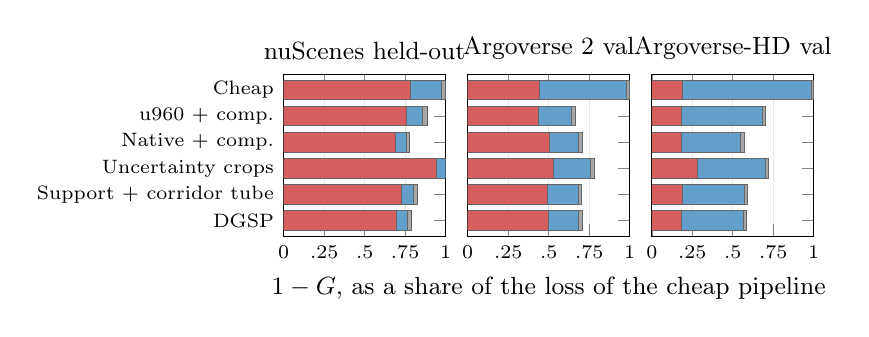
\begin{tikzpicture}
\begin{groupplot}[group style={group size=3 by 1, horizontal sep=8pt, yticklabels at=edge left},
  width=0.30\linewidth, height=0.30\linewidth, xbar stacked, /pgf/bar width=7pt,
  xmin=0, xmax=1.0, xtick={0,0.25,0.5,0.75,1}, xticklabels={0,.25,.5,.75,1},
  ymin=-0.6, ymax=5.6, ytick={0,...,5}, y dir=reverse,
  yticklabels={{Cheap},{u960 + comp.},{Native + comp.},{Uncertainty crops},{Support + corridor tube},{DGSP}},
  tick label style={font=\scriptsize}, label style={font=\small}, title style={font=\small, yshift=-4pt},
  xmajorgrids, grid style={gray!20},
  legend style={font=\scriptsize, draw=gray!50, column sep=4pt}, legend cell align=left]
\nextgroupplot[title={nuScenes held-out}, legend to name=losslegend, legend columns=3]
\addplot[fill=oursc!75, draw=black!60, line width=0.3pt] coordinates {(0.782,0) (0.756,1) (0.692,2) (0.943,3) (0.727,4) (0.696,5)};
\addlegendentry{insufficient braking}
\addplot[fill=adac!70, draw=black!60, line width=0.3pt] coordinates {(0.191,0) (0.102,1) (0.067,2) (0.079,3) (0.075,4) (0.071,5)};
\addlegendentry{excessive braking}
\addplot[fill=black!35, draw=black!60, line width=0.3pt] coordinates {(0.027,0) (0.030,1) (0.019,2) (0.037,3) (0.024,4) (0.022,5)};
\addlegendentry{command changes, collisions}
\nextgroupplot[title={Argoverse~2 val}, xlabel={$1-\G$, as a share of the loss of the cheap pipeline}]
\addplot[fill=oursc!75, draw=black!60, line width=0.3pt] coordinates {(0.443,0) (0.437,1) (0.506,2) (0.527,3) (0.495,4) (0.498,5)};
\addplot[fill=adac!70, draw=black!60, line width=0.3pt] coordinates {(0.534,0) (0.205,1) (0.177,2) (0.233,3) (0.187,4) (0.187,5)};
\addplot[fill=black!35, draw=black!60, line width=0.3pt] coordinates {(0.023,0) (0.020,1) (0.023,2) (0.021,3) (0.022,4) (0.022,5)};
\nextgroupplot[title={Argoverse-HD val}]
\addplot[fill=oursc!75, draw=black!60, line width=0.3pt] coordinates {(0.192,0) (0.180,1) (0.182,2) (0.279,3) (0.187,4) (0.184,5)};
\addplot[fill=adac!70, draw=black!60, line width=0.3pt] coordinates {(0.793,0) (0.503,1) (0.367,2) (0.421,3) (0.386,4) (0.379,5)};
\addplot[fill=black!35, draw=black!60, line width=0.3pt] coordinates {(0.015,0) (0.021,1) (0.022,2) (0.018,3) (0.019,4) (0.019,5)};
\end{groupplot}
\end{tikzpicture}

\vspace{2pt}
\pgfplotslegendfromname{losslegend}
\caption{\textbf{Which part of the decision loss does \method remove?} Decision loss split into insufficient braking, excessive braking, and command changes and collisions, as a share of the total loss of the cheap pipeline; the length of a bar is $1-\G$. All pipelines except the cheap one use the shared components. Values in \cref{tab:loss}.}
\label{fig:loss}
\end{figure}

\Cref{tab:loss} decomposes the decision loss.
Relative to the cheap detector, \method removes most of the loss of excessive braking, and its loss of insufficient braking is close to that of native-resolution inference with the same components on all three datasets; the paired intervals of the difference per frame, $\ci{-0.055}{+0.049}$, $\ci{-0.074}{+0.052}$, and $\ci{-0.013}{+0.015}$, include zero.
\method also takes fewer unnecessary braking actions than whole-frame inference at any resolution on the three datasets, also when the latter is given its components ($15$, $53$, and $131$ per $1{,}000$ frames, compared with $42$, $126$, and $265$ for u960 and at least $17$, $56$, and $142$ with the components), and on nuScenes, it delays the onset of hard braking on $1.7$ frames per $1{,}000$, compared with $7.8$ for the cheap detector ($\ci{-12.65}{-1.74}$).

% --- Table: detection metrics (handoff/K30/v7_detection.csv) ---
\begin{table}[!tbp]
\centering
\caption{\textbf{Detection metrics.} \method attains the highest precision on the decision-relevant objects on all three datasets. ``Relevant'': the decision-relevant objects of \cref{sec:supp_metric}; ``Spurious'': detections per $1{,}000$ frames that trigger braking without a corresponding object. Whole frame with the shared components.}
\label{tab:det}
\small
\setlength{\tabcolsep}{3.2pt}
\begin{tabular}{@{}lcccc@{}}
\toprule
 & & \multicolumn{2}{c}{Relevant} & \\
\cmidrule(lr){3-4}
Pipeline & AP$_{50}\uparrow$ & Recall$\,\uparrow$ & Prec.$\,\uparrow$ & Spurious$\,\downarrow$ \\
\midrule
\multicolumn{5}{@{}l}{\emph{nuScenes held-out}} \\
Cheap (u320) & 0.148 & 0.759 & 0.505 & 16.6 \\
u960 & 0.246 & 0.859 & 0.665 & 7.6 \\
Native & 0.245 & 0.848 & 0.731 & 4.2 \\
Support + ego corridor & 0.170 & 0.821 & 0.780 & \best{3.8} \\
\oursrow \textbf{\method} & 0.162 & 0.824 & \best{0.799} & \best{3.8} \\
\midrule
\multicolumn{5}{@{}l}{\emph{Argoverse~2 val}} \\
Cheap (u320) & 0.107 & 0.804 & 0.466 & 16.3 \\
u960 & 0.178 & 0.909 & 0.677 & 8.7 \\
Native & 0.184 & 0.919 & 0.665 & 14.8 \\
Support + ego corridor & 0.119 & 0.900 & 0.714 & 5.9 \\
\oursrow \textbf{\method} & 0.115 & 0.901 & \best{0.719} & \best{5.6} \\
\midrule
\multicolumn{5}{@{}l}{\emph{Argoverse-HD val}} \\
Cheap (u320) & 0.117 & 0.664 & 0.312 & 27.7 \\
u960 & 0.199 & 0.909 & 0.410 & 44.3 \\
Native & 0.202 & 0.923 & 0.456 & 16.2 \\
Support + ego corridor & 0.118 & 0.883 & 0.491 & \best{14.7} \\
\oursrow \textbf{\method} & 0.130 & 0.890 & \best{0.511} & 15.0 \\
\bottomrule
\end{tabular}
\end{table}

\noindent\textbf{Detection metrics.}
On the decision-relevant objects, \method attains the highest precision on all three datasets, and it produces $50\%$, $64\%$, and $34\%$ of the spurious braking detections of whole-frame inference at the verification resolution.
The whole-image AP is not the objective of the method, since objects that cannot affect the action are not re-detected.

\subsection{Other detectors}
\label{sec:supp_detectors}

% --- Table: second detector family (handoff/K28 phase3/ctable_y11s.csv) ---
\begin{table}[!tbp]
\centering
\caption{\textbf{YOLO11s as the cheap and the reference detector} (unchanged configurations). Upper rows: whole frame with the refiner only; ``+ looming'': whole frame with the full lift, as \method. $^{\dagger}$ / $^{\ast}$: \method is significantly better / worse.}
\label{tab:det2}
\small
\setlength{\tabcolsep}{3pt}
\begin{tabular}{@{}lcccccc@{}}
\toprule
 & \multicolumn{2}{c}{nuScenes} & \multicolumn{2}{c}{Argoverse 2} & \multicolumn{2}{c}{Argoverse-HD} \\
\cmidrule(lr){2-3}\cmidrule(lr){4-5}\cmidrule(l){6-7}
Pipeline & $\G\uparrow$ & px\,(\%) & $\G\uparrow$ & px\,(\%) & $\G\uparrow$ & px\,(\%) \\
\midrule
u640 & 0.319$^{\dagger}$ & 17.1 & 0.145$^{\dagger}$ & 10.3 & 0.079$^{\dagger}$ & 11.6 \\
u960 & 0.408 & 38.4 & 0.158$^{\dagger}$ & 23.2 & 0.111$^{\dagger}$ & 25.3 \\
u1280 & 0.434 & 65.4 & 0.145$^{\dagger}$ & 40.0 & 0.101$^{\dagger}$ & 44.4 \\
Native & 0.410 & 103.1 & 0.085$^{\dagger}$ & 101.2 & 0.119$^{\dagger}$ & 101.3 \\
\midrule
u512 + looming & 0.309 & 10.2 & 0.310 & 6.7 & 0.277$^{\dagger}$ & 7.1 \\
u640 + looming & 0.379 & 17.1 & 0.316$^{\ast}$ & 10.3 & 0.300$^{\dagger}$ & 11.6 \\
u960 + looming & 0.446 & 38.4 & 0.323$^{\ast}$ & 23.2 & 0.300$^{\dagger}$ & 25.3 \\
u1280 + looming & 0.483$^{\ast}$ & 65.4 & 0.311 & 40.0 & 0.316$^{\dagger}$ & 44.4 \\
Native + looming & 0.443 & 103.1 & 0.260 & 101.2 & 0.412 & 101.3 \\
\midrule
Hand-crafted looming & 0.410 & 7.7 & 0.246 & 5.4 & 0.362 & 6.9 \\
\oursrow \textbf{\method} & 0.418 & 7.7 & \best{0.261} & 5.4 & \best{0.422} & 6.9 \\
\bottomrule
\end{tabular}
\end{table}

\Cref{tab:det2} repeats the comparison with YOLO11s~\cite{yolo11} as the cheap and the reference detector; the configurations are unchanged, and the refiner and the looming estimate, which were trained on YOLOv8s boxes, are applied without retraining.
Against whole-frame inference with the refiner only, \method is significantly better at every resolution on Argoverse~2 and Argoverse-HD.
With the full lift on both sides, this holds only on Argoverse-HD (up to $1280$ pixels; native ties): whole-frame inference is significantly better than \method at $1280$ pixels on nuScenes and at $640$ and $960$ pixels on Argoverse~2, with $1.9$--$8.5\times$ its pixels, and no other difference on these two datasets is significant.
The pattern is that of YOLOv8s (\cref{tab:uniform}).

\begin{table}[!htbp]
\centering
\begin{minipage}[t]{0.44\linewidth}
\centering
% --- Table: fine-tuned detectors on nuScenes (handoff/K28 phase3/ctable_ft0.csv, ctable_ft1.csv; zoom-based detectors: K12) ---
\caption{\textbf{Decision value on nuScenes held-out with detectors fine-tuned on the training split} (two training seeds). ``+ comp.'': with the refiner and the learned looming estimate of \method.}
\label{tab:ft}
\small
\setlength{\tabcolsep}{6pt}
\begin{tabular}{@{}lcc@{}}
\toprule
Method (fine-tuned) & Seed 0 & Seed 1 \\
\midrule
u960 & 0.241 & 0.272 \\
u960 + comp. & 0.328 & 0.356 \\
FOVEA~\cite{fovea} & 0.235 & 0.244 \\
LZU~\cite{lzu} & 0.219 & 0.184 \\
UFP~\cite{ufpmp} & 0.202 & 0.180 \\
ESOD~\cite{esod} & 0.221 & 0.229 \\
ZoomDet~\cite{zoomdet} & 0.259 & 0.235 \\
\midrule
\method w/o refiner & 0.336 & 0.336 \\
\oursrow \textbf{\method} & \best{0.359} & \best{0.364} \\
\bottomrule
\end{tabular}
\end{minipage}\hfill
\begin{minipage}[t]{0.53\linewidth}
\centering
% --- Table: fine-tuned regime on Argoverse 2 (handoff/K33/ft_rows.csv) ---
\caption{\textbf{Decision value on Argoverse~2 val with detectors fine-tuned on Argoverse~2 train} (one seed). ``Official'': monocular lift of~\cite{deep}; ``+ looming'': with the learned looming estimate; ``+ looming + ref.'': also with the range refiner. $^{\dagger}$: \method significantly better.}
\label{tab:ft_av2}
\small
\setlength{\tabcolsep}{4pt}
\begin{tabular}{@{}lccc@{}}
\toprule
Method (fine-tuned) & Official & + looming & + looming + ref. \\
\midrule
u960 & $-$0.473$^{\dagger}$ & $-$0.126$^{\dagger}$ & $-$0.063$^{\dagger}$ \\
FOVEA~\cite{fovea} & $-$0.503$^{\dagger}$ & $-$0.126$^{\dagger}$ & $-$0.080$^{\dagger}$ \\
LZU~\cite{lzu} & $-$0.526$^{\dagger}$ & $-$0.125$^{\dagger}$ & $-$0.080$^{\dagger}$ \\
UFP~\cite{ufpmp} & \na & $-$0.087$^{\dagger}$ & $-$0.009$^{\dagger}$ \\
ESOD~\cite{esod} & $-$0.736$^{\dagger}$ & $-$0.175$^{\dagger}$ & $-$0.120$^{\dagger}$ \\
ZoomDet~\cite{zoomdet} & $-$0.384$^{\dagger}$ & $-$0.084$^{\dagger}$ & $-$0.035$^{\dagger}$ \\
\midrule
\oursrow \textbf{\method} & \na & 0.144$^{\dagger}$ & \best{0.224} \\
\bottomrule
\end{tabular}
\end{minipage}
\end{table}

\noindent\textbf{Fine-tuned detectors.}
In \cref{tab:ft}, \method uses the fine-tuned detector for verification, and the refiner and the looming estimate are applied without retraining.
It attains the highest decision value for both seeds, also compared with fine-tuned whole-frame inference that is given its components at any resolution (at most $0.328$ and $0.356$); the differences to the latter are significant at long sides of $448$, $512$, $1280$, and $1536$ pixels for seed~0 and of $448$, $1536$, and $1600$ pixels for seed~1.

On Argoverse~2 (\cref{tab:ft_av2}), \method with the fine-tuned verifier attains $0.224$ and significantly outperforms every fine-tuned detector in every form, with lower interval bounds of at least $0.14$, whereas all of them attain lower decision values than the cheap COCO-pretrained detector, also with the shared components.
The fine-tuned detectors learn the projected cuboid boxes of the annotations, which are larger than the tight boxes of COCO; the estimated range of the decisive object is shorter (median ratio $0.96$--$0.97$ relative to u960 with the COCO-pretrained detector), and with the components, u960, FOVEA, LZU, UFP, and ZoomDet brake hard on $8.1$--$13.8\%$ of the frames that require no braking, compared with $5.0\%$ for \method; ESOD brakes less often but misses the decisive object more often.
\method is affected least, since it verifies only the regions the decision requires and retains the geometry of the COCO-pretrained draft elsewhere.

%%%%%%%%%%%%%%%%%%%%%%%%%%%%%%%%%%%%%%%%%%%%%%%%%%%%%%%%%%%%%%%%%%%%%%%%%%%%%%
%% S4. UNSEEN OBJECTS, FIELD BEHAVIOUR, COVERAGE
%%%%%%%%%%%%%%%%%%%%%%%%%%%%%%%%%%%%%%%%%%%%%%%%%%%%%%%%%%%%%%%%%%%%%%%%%%%%%%
\section{Unseen-object recovery, field behavior, and coverage}
\label{sec:supp_field}

This section examines the first mechanism of \method, the search for objects that the draft misses: how many such objects it recovers (\cref{sec:supp_missed}), how often the verified region contains the object that decides the action (\cref{sec:supp_coverage}), and how the field differs from a fixed region that has the same pixels (\cref{sec:supp_tube}).

\subsection{Recovery of objects missing from the draft}
\label{sec:supp_missed}

On the frames in which braking is required but the draft contains no object that supports braking ($3.0$--$5.7\%$ of the frames), \method attains $\G=0.33$, $0.29$, and $0.68$ on nuScenes, Argoverse~2, and Argoverse-HD, compared with $0$ for the support alone and at most $0.17$ for uncertainty crops.

% --- Table: missed objects (handoff/K28 phase3/missed_natural_v6.csv, missed_controlled_v6.csv, regime_v6.csv) ---
\begin{table}[!tbp]
\centering
\caption{\textbf{Decision-relevant objects that are missing from the draft.} ``Nat.'': recovery of the objects that the cheap detector misses and u960 detects. ``Del.'': recovery after the draft detections of all relevant objects are deleted, with the detector-input pixels in this setting. ``Reg.'': decision value on the frames in which braking is required but the draft contains no supporting object. All policies use the refiner and the learned looming estimate.}
\label{tab:missed}
\footnotesize
\setlength{\tabcolsep}{3.4pt}
\begin{tabular}{@{}lcccccccccccccc@{}}
\toprule
 & \multicolumn{4}{c}{nuScenes} & & \multicolumn{4}{c}{Argoverse 2} & & \multicolumn{4}{c}{Argoverse-HD} \\
\cmidrule(lr){2-5}\cmidrule(lr){7-10}\cmidrule(l){12-15}
Policy & Nat. & Del. & px\,(\%) & Reg. & & Nat. & Del. & px\,(\%) & Reg. & & Nat. & Del. & px\,(\%) & Reg. \\
\midrule
Support only & 0.197 & 0.149 & 5.6 & 0.000 &  & 0.379 & 0.192 & 4.1 & 0.000 &  & 0.201 & 0.237 & 6.8 & 0.000 \\
Uncertainty crops & 0.256 & 0.399 & 16.5 & 0.061 &  & 0.510 & 0.566 & 12.8 & 0.151 &  & 0.473 & 0.637 & 16.6 & 0.167 \\
Field only & 0.453 & 0.792 & 11.7 & 0.329 &  & 0.540 & 0.754 & 6.0 & 0.224 &  & 0.738 & 0.654 & 5.8 & 0.678 \\
AnA-style, one pass & \best{0.718} & 0.447 & \na & \na &  & 0.801 & 0.534 & \na & \na &  & 0.866 & 0.558 & \na & \na \\
AnA-style, iterated & \best{0.718} & 0.451 & \na & \na &  & 0.808 & 0.559 & \na & \na &  & 0.865 & 0.574 & \na & \na \\
Counterfactual, one pass & 0.205 & 0.191 & \na & \na &  & 0.419 & 0.237 & \na & \na &  & 0.202 & 0.251 & \na & \na \\
Counterfactual, iterated & 0.214 & 0.197 & \na & \na &  & 0.427 & 0.251 & \na & \na &  & 0.206 & 0.268 & \na & \na \\
\oursrow \textbf{\method} & 0.607 & \best{0.847} & 14.1 & \best{0.331} &  & \best{0.848} & \best{0.876} & 8.6 & \best{0.289} &  & \best{0.873} & \best{0.846} & 10.3 & \best{0.684} \\
\bottomrule
\end{tabular}
\end{table}

The field accounts for most of the recovered objects, and the support adds the objects that lie within the crops of draft detections; their combination recovers more objects than uncertainty crops with fewer pixels on all three datasets.
After the deletion, AnA-style refinement recovers at most $57\%$ and counterfactual importance at most $27\%$ of these objects, since neither selects regions by probing hypothetical unseen objects; their recovery depends on whether a missed object falls within crops selected from the remaining draft detections.

\noindent\textbf{Natural misses on nuScenes.}
Of the natural misses of \cref{tab:missed} on nuScenes, $78$ of $117$ have a draft box with a confidence between $0.05$ and $0.25$, which AnA-style refinement verifies and \method, with the draft threshold of $0.25$ of all other pipelines, does not; on these objects, AnA-style refinement recovers $0.85$ and \method $0.60$, whereas on the others, \method recovers more ($0.62$ \vs $0.46$).
On Argoverse~2 and Argoverse-HD, the field footprint of \method recovers more of the natural misses inside it ($0.93$ \vs $0.77$ and $0.86$) and recovers more overall; the two signals are complementary.

% --- K40-5 / D06 (handoff/K40R/k40_5_lowconf.csv, k40_5_lowconf_checks.json; post-hoc variant on the test split) ---
\noindent\textbf{Low-confidence draft boxes.}
A post-hoc variant, evaluated only on the nuScenes held-out split and not used elsewhere, tests whether this gap is due to the draft threshold.
It runs one additional cheap pass at a confidence of $0.05$ and adds the boxes with a confidence between $0.05$ and $0.25$ that lie in the ego corridor and do not duplicate a draft box to the requests of the first round, leaving the loop unchanged; this seeds $7{,}377$ crops on $42\%$ of the frames.
The variant raises the decision value from $0.211$ to $0.231$ ($\Delta=-0.020$, $\ci{-0.038}{-0.002}$), the repair rate from $0.734$ to $0.781$, and the share of the $270$ annotated decision-relevant objects that the cheap detector misses and the pipeline finds from $0.31$ to $0.43$, at $1.9\times$ the pixels ($1.4\times$ without the additional pass).
Part of the gap to AnA-style refinement on natural misses is therefore a property of the draft threshold rather than of the field; since the variant was formed after the test results were known, we report it as a direction, not as a result of \method.

\subsection{Coverage of the decisive object}
\label{sec:supp_coverage}

\begin{figure}[!htbp]
\centering
% plot generated from the reference tables (script: versions/paper_tools_2026-10-27/make_supp_figs.py)
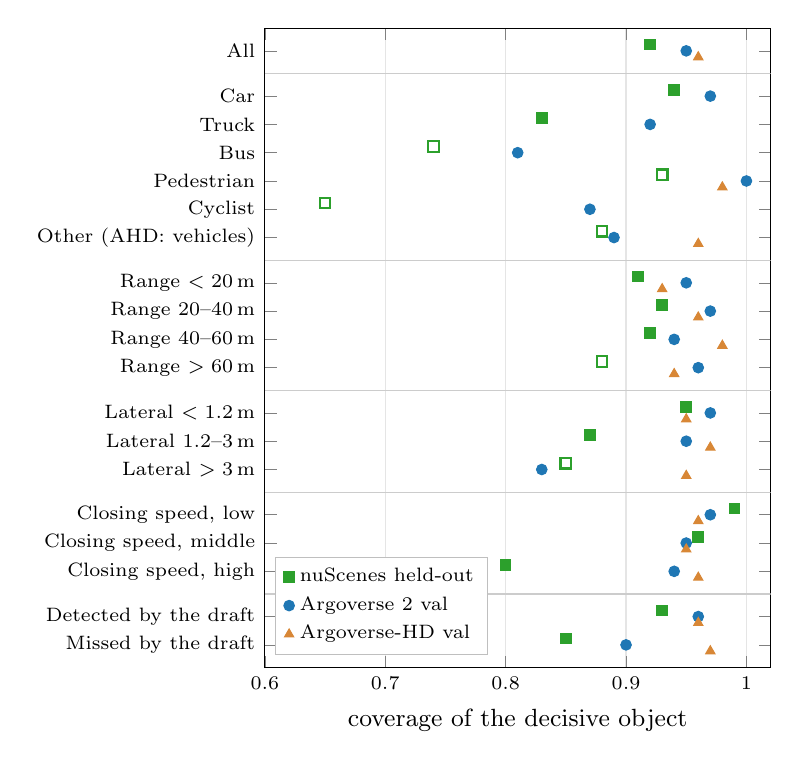
\begin{tikzpicture}
\begin{axis}[width=0.66\linewidth, height=0.80\linewidth, xmin=0.6, xmax=1.02,
  ymin=-0.8, ymax=21.8, y dir=reverse, ytick={0.0,1.6,2.6,3.6,4.6,5.6,6.6,8.2,9.2,10.2,11.2,12.8,13.8,14.8,16.4,17.4,18.4,20.0,21.0},
  yticklabels={{All},{Car},{Truck},{Bus},{Pedestrian},{Cyclist},{Other (AHD: vehicles)},{Range $<20$\,m},{Range $20$--$40$\,m},{Range $40$--$60$\,m},{Range $>60$\,m},{Lateral $<1.2$\,m},{Lateral $1.2$--$3$\,m},{Lateral $>3$\,m},{Closing speed, low},{Closing speed, middle},{Closing speed, high},{Detected by the draft},{Missed by the draft}},
  xtick={0.6,0.7,0.8,0.9,1.0}, tick label style={font=\scriptsize}, label style={font=\small},
  xlabel={coverage of the decisive object}, xmajorgrids, grid style={gray!20},
  legend style={font=\scriptsize, at={(0.02,0.02)}, anchor=south west, draw=gray!50}, legend cell align=left]
\draw[gray!40] (axis cs:0.6,0.80) -- (axis cs:1.02,0.80);
\draw[gray!40] (axis cs:0.6,7.40) -- (axis cs:1.02,7.40);
\draw[gray!40] (axis cs:0.6,12.00) -- (axis cs:1.02,12.00);
\draw[gray!40] (axis cs:0.6,15.60) -- (axis cs:1.02,15.60);
\draw[gray!40] (axis cs:0.6,19.20) -- (axis cs:1.02,19.20);
\addplot[cropc, only marks, mark=square*, mark size=1.9pt] coordinates {(0.92,-0.22) (0.94,1.38) (0.83,2.38) (0.91,7.98) (0.93,8.98) (0.92,9.98) (0.95,12.58) (0.87,13.58) (0.99,16.18) (0.96,17.18) (0.80,18.18) (0.93,19.78) (0.85,20.78)};
\addlegendentry{nuScenes held-out}
\addplot[cropc, only marks, mark=square, mark size=1.9pt, thick, forget plot] coordinates {(0.74,3.38) (0.93,4.38) (0.65,5.38) (0.88,6.38) (0.88,10.98) (0.85,14.58)};
\addplot[adac, only marks, mark=*, mark size=1.9pt] coordinates {(0.95,0.00) (0.97,1.60) (0.92,2.60) (0.81,3.60) (1.00,4.60) (0.87,5.60) (0.89,6.60) (0.95,8.20) (0.97,9.20) (0.94,10.20) (0.96,11.20) (0.97,12.80) (0.95,13.80) (0.83,14.80) (0.97,16.40) (0.95,17.40) (0.94,18.40) (0.96,20.00) (0.90,21.00)};
\addlegendentry{Argoverse~2 val}
\addplot[fieldc!90!black, only marks, mark=triangle*, mark size=1.9pt] coordinates {(0.96,0.22) (0.98,4.82) (0.96,6.82) (0.93,8.42) (0.96,9.42) (0.98,10.42) (0.94,11.42) (0.95,13.02) (0.97,14.02) (0.95,15.02) (0.96,16.62) (0.95,17.62) (0.96,18.62) (0.96,20.22) (0.97,21.22)};
\addlegendentry{Argoverse-HD val}
\end{axis}
\end{tikzpicture}
\caption{\textbf{Where does the verified region miss the decisive object?} Share of the frames that require braking on which the decisive object lies in the verified region of \method (field footprint, support and guard crops accumulated up to the final round), by stratum. Coverage is box-center geometry, not detection recall. Hollow markers: strata with fewer than $30$ frames. On Argoverse-HD, the annotations do not separate vehicle classes. Values and frame counts in \cref{tab:coverage}.}
\label{fig:coverage}
\end{figure}

\Cref{tab:coverage} breaks down whether the decisive object of a frame that requires braking lies in the verified region.
It is $0.92$ $\ci{0.88}{0.95}$, $0.95$ $\ci{0.94}{0.97}$, and $0.96$ $\ci{0.92}{0.98}$ overall ($0.90$ $\ci{0.85}{0.93}$, $0.92$ $\ci{0.90}{0.95}$, and $0.91$ $\ci{0.81}{0.97}$ with the field and support crops alone, \ie, on the verified region $R$ without the guard crops) and lowest for objects more than $3$\,m from the ego lane ($0.85$ and $0.83$ on nuScenes and Argoverse~2), for objects that the draft misses ($0.85$ and $0.90$), and, on nuScenes, for the third of the objects with the highest closing speed ($0.80$ $\ci{0.73}{0.87}$), which the static probe ($\vclose=0$) of the deployed configuration does not anticipate.
The deployable probe changes of \cref{tab:locality} (closing probe, extended grid, three sizes) with real crop detections raise the coverage of this tercile to $0.997$ and the overall coverage to $0.999$, $0.976$, and $0.962$, at $2.0$--$2.4\times$ the pixels; the decision value changes by $+0.031$ $\ci{-0.007}{+0.074}$, $+0.031$ $\ci{-0.007}{+0.081}$, and $-0.092$ $\ci{-0.278}{-0.003}$, so that the deployed probe is a deliberate trade-off between coverage and compute.
Classes with fewer than $30$ frames (buses and cyclists on nuScenes) have wide intervals.

\subsection{Field and fixed tube}
\label{sec:supp_tube}

\begin{table}[!htbp]
\centering
% --- Table: field vs fixed tube (handoff/K30/v8d_speed.csv, v2_tube.csv) ---
\caption{\textbf{The field adapts to the ego speed} (nuScenes held-out; the braking demand is recomputed with the ego speed scaled). Range: farthest sensitive range of the field (mean over frames with a non-empty field); Field: mean image area of the field footprint (\% of the frame); px and $\G$: \method / hybrid (support + ego-corridor tube). $\Delta$: $95\%$ interval of (\method$\,-\,$hybrid).}
\label{tab:speed}
\small
\setlength{\tabcolsep}{2.6pt}
\begin{tabular}{@{}lccccc@{}}
\toprule
Ego speed & Range & Field\,(\%) & px\,(\%) & $\G$ & $\Delta$ \\
\midrule
$\times0.5$ & 14\,m & 1.7 & 5.5 / 6.4 & 0.241 / 0.237 & \ci{-0.001}{+0.011} \\
$\times1.0$ & 28\,m & 5.6 & 7.8 / 10.8 & 0.211 / 0.174 & \ci{-0.012}{+0.096} \\
$\times1.5$ & 43\,m & 6.5 & 8.6 / 12.2 & 0.196 / 0.153 & \best{\ci{+0.003}{+0.087}} \\
\bottomrule
\end{tabular}
\end{table}

\begin{table}[!htbp]
\centering
% --- Table: curved-path braking consumer (handoff/K31/curv_test.csv) ---
\caption{\textbf{Braking controller with a curved corridor} that follows the path of constant curvature given by the ego yaw rate (decision value under this planner). $^{\dagger}$ / $^{\ast}$: \method significantly better / worse. The hybrid with a curved support and tube knows the path and serves as a path-aware hand-crafted comparator.}
\label{tab:curved}
\small
\setlength{\tabcolsep}{3pt}
\begin{tabular}{@{}lccc@{}}
\toprule
Pipeline & nuScenes & Argoverse 2 & Argov.-HD \\
\midrule
u960 + comp. & 0.101 & 0.276$^{\ast}$ & 0.282$^{\dagger}$ \\
Native + comp. & 0.235 & 0.225 & 0.422 \\
Uncertainty crops & $-$0.083$^{\dagger}$ & 0.168 & 0.255$^{\dagger}$ \\
Support + straight tube & 0.154 & 0.209 & 0.352$^{\dagger}$ \\
Curved support + curved tube & 0.186 & 0.200 & 0.379 \\
\method, straight controller & 0.227 & 0.254 & 0.334$^{\dagger}$ \\
\midrule
\oursrow \textbf{\method, curved controller} & 0.207 & 0.224 & 0.394 \\
\bottomrule
\end{tabular}
\end{table}

% --- Table: second consumer (handoff/K28 phase3/consumer2_v6.csv, refiner v3a in all rows) ---
\begin{table}[!tbp]
\centering
\caption{\textbf{Time-to-collision warning as a second max-composable planner} (decision value; detector-input pixels in \% in parentheses). All pipelines use the refiner and the learned looming estimate.}
\label{tab:consumer2}
\small
\setlength{\tabcolsep}{2.4pt}
\begin{tabular}{@{}lccc@{}}
\toprule
Pipeline & nuScenes & Argoverse 2 & Argov.-HD \\
\midrule
u960 & 0.157 (38.4) & 0.448 (23.2) & 0.326 (25.3) \\
Native & 0.222 (103.1) & 0.499 (101.2) & 0.629 (101.3) \\
Uncertainty crops & 0.187 (11.6) & 0.418 (9.2) & 0.672 (14.3) \\
Support + ego-corridor tube & 0.146 (10.9) & 0.427 (6.9) & 0.616 (11.0) \\
Support + tube, capped & 0.157 (12.4) & 0.473 (7.7) & 0.724 (12.8) \\
\oursrow \textbf{\method} & 0.191 (8.6) & 0.496 (6.0) & \best{0.750} (7.9) \\
\bottomrule
\end{tabular}
\end{table}

% --- K40-4/7 (handoff/K40R/FIELD_EQUIVALENCE.md, k40_4_7_summary_*.csv) and K40-6 / D02 (handoff/K40R/k40_6_speed_tubes.csv; refiner v3a) ---
\begin{table}[!htbp]
\centering
\caption{\textbf{Field \vs action-independent stopping-distance tubes.} The tube covers the ego corridor up to the range $2+0.4v+v^2/(2\tau)$ at the ego speed $v$ for a fixed $\tau$: the threshold of \textsc{decelerate} ($\tau_1$), \ie, the field at \textsc{keep} applied at every action, or that of \textsc{hard-brake} ($\tau_2$), \ie, the field at \textsc{decelerate}. Support, components, crop scale, guard, and merge rule are those of \method. Caps as in \cref{sec:supp_heuristics}; ``strict, diag.'': a diagnostic variant of the strict cap that also removes regions whose verification was denied from the observed region. px: pixels relative to \method; $\Delta$: \method minus the row.}
\label{tab:speedtube}
\small
\setlength{\tabcolsep}{2.4pt}
\begin{tabular}{@{}lcccccccc@{}}
\toprule
 & \multicolumn{2}{c}{nuScenes held-out} & & \multicolumn{2}{c}{Argoverse~2 val} & & \multicolumn{2}{c}{Argoverse-HD val} \\
\cmidrule(lr){2-3}\cmidrule(lr){5-6}\cmidrule(l){8-9}
Tube (cap) & $\G$ (px) & $\Delta$ & & $\G$ (px) & $\Delta$ & & $\G$ (px) & $\Delta$ \\
\midrule
$\tau_1$, nominal & 0.154 (1.03) & \best{\ci{+0.004}{+0.117}} & & 0.285 (1.10) & \ci{-0.008}{+0.026} & & 0.411 (1.06) & \best{\ci{+0.002}{+0.013}} \\
$\tau_1$, strict & 0.148 (0.98) & \best{\ci{+0.006}{+0.123}} & & 0.248 (0.96) & \best{\ci{+0.012}{+0.080}} & & 0.429 (0.92) & \ci{-0.039}{+0.016} \\
$\tau_1$, strict, diag. & 0.148 (0.98) & \best{\ci{+0.006}{+0.124}} & & 0.256 (0.96) & \best{\ci{+0.011}{+0.068}} & & 0.402 (0.92) & \best{\ci{+0.009}{+0.022}} \\
$\tau_2$, nominal & 0.140 (0.80) & \best{\ci{+0.016}{+0.131}} & & 0.271 (0.93) & \best{\ci{+0.003}{+0.042}} & & 0.408 (0.90) & \best{\ci{+0.003}{+0.015}} \\
$\tau_2$, strict & 0.141 (0.79) & \best{\ci{+0.016}{+0.131}} & & 0.272 (0.90) & \best{\ci{+0.001}{+0.042}} & & 0.417 (0.88) & \ci{-0.011}{+0.011} \\
$\tau_2$, strict, diag. & 0.141 (0.79) & \best{\ci{+0.016}{+0.131}} & & 0.267 (0.90) & \best{\ci{+0.007}{+0.048}} & & 0.407 (0.88) & \best{\ci{+0.004}{+0.018}} \\
\midrule
\oursrow \textbf{\method} & \textbf{0.211} (1) & \na & & \textbf{0.294} (1) & \na & & 0.418 (1) & \na \\
\bottomrule
\end{tabular}
\end{table}

% --- Fig.: field vs fixed tube by draft action (handoff/K36b: f1 panels a/b = k36b.py BEV renders, frames by fixed time-order rules;
%     bars = f2_groups.csv pooled over speed bins, weighted by frames; all three test splits) ---
\begin{figure}[!htbp]
\centering
\begin{minipage}{0.55\linewidth}\centering
\begin{minipage}[c]{0.19\linewidth}\centering
{\footnotesize\textsc{keep}}\\[1pt]\includegraphics[width=0.88\linewidth]{figs/t_keep_bev.pdf}\\[3pt]
{\footnotesize\textsc{decel.}}\\[1pt]\includegraphics[width=0.88\linewidth]{figs/t_decel_bev.pdf}
\end{minipage}\hfill
\begin{minipage}[c]{0.79\linewidth}\centering
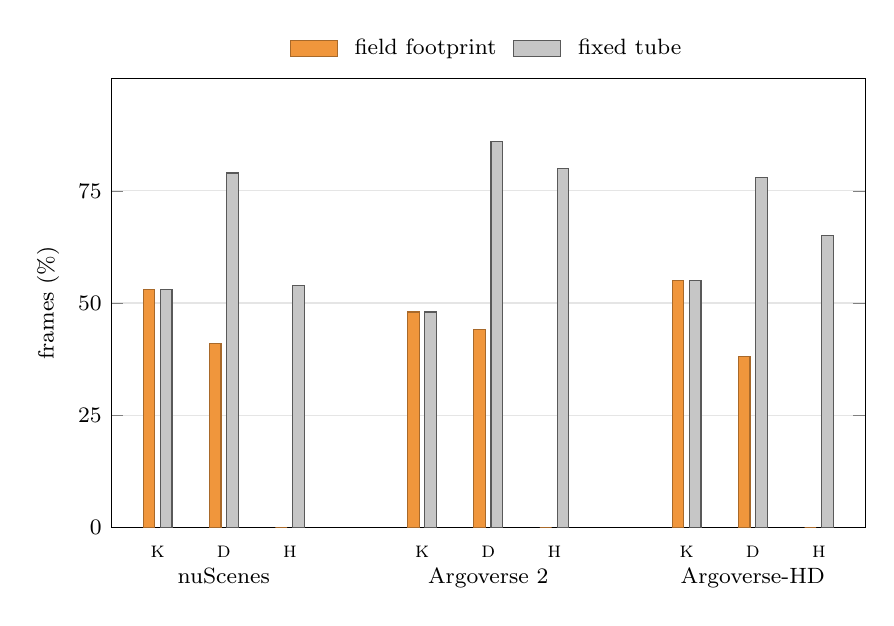
\begin{tikzpicture}
\begin{axis}[
  width=0.92\linewidth, height=0.60\linewidth,
  ybar, bar width=4.2pt, ymin=0, ymax=1.0, enlarge x limits=0.07, area legend,
  symbolic x coords={nK,nD,nH,g1,aK,aD,aH,g2,hK,hD,hH},
  xtick={nK,nD,nH,aK,aD,aH,hK,hD,hH}, xticklabels={\textsc{k},\textsc{d},\textsc{h},\textsc{k},\textsc{d},\textsc{h},\textsc{k},\textsc{d},\textsc{h}}, xtick style={draw=none}, xticklabel style={yshift=1pt},
  ytick={0,0.25,0.5,0.75}, yticklabels={0,25,50,75},
  ylabel={frames (\%)}, tick label style={font=\footnotesize}, label style={font=\footnotesize},
  ymajorgrids, grid style={gray!20},
  legend style={font=\footnotesize, at={(0.5,1.02)}, anchor=south, legend columns=2, draw=none, column sep=4pt},
  clip=false,
]
\addplot[fill=fieldc, draw=fieldc!70!black] coordinates {(nK,0.53) (nD,0.41) (nH,0) (aK,0.48) (aD,0.44) (aH,0) (hK,0.55) (hD,0.38) (hH,0)};
\addlegendentry{field footprint}
\addplot[fill=gray!45, draw=gray!70!black] coordinates {(nK,0.53) (nD,0.79) (nH,0.54) (aK,0.48) (aD,0.86) (aH,0.80) (hK,0.55) (hD,0.78) (hH,0.65)};
\addlegendentry{fixed tube}
\node[font=\footnotesize, anchor=north, yshift=-11.5pt] at (axis cs:nD,0) {nuScenes};
\node[font=\footnotesize, anchor=north, yshift=-11.5pt] at (axis cs:aD,0) {Argoverse~2};
\node[font=\footnotesize, anchor=north, yshift=-11.5pt] at (axis cs:hD,0) {Argoverse-HD};
\end{axis}
\end{tikzpicture}
\end{minipage}
\end{minipage}
\caption{\textbf{The field depends on the action, the tube does not.} Left: field (orange) and tube of the hybrid (dashed) at the draft actions \textsc{keep} and \textsc{decelerate} (nuScenes). Right: share of the evaluated frames with draft action \textsc{keep} (K), \textsc{decelerate} (D), or \textsc{hard-brake} (H) on which each requests pixels.}
\label{fig:tube}
\end{figure}

\noindent\textbf{The field as an action-adaptive corridor.}
For the braking controller and a static probe, a cell is sensitive exactly when the demand of an object there reaches the threshold $\tau_{a+1}$ of the next stronger action and its lateral extent overlaps the corridor, which reduces to a range below $2+0.4v+v^2/(2\tau_{a+1})$, the stopping distance at that deceleration with the reaction time and margin of the planner, and to the empty set at \textsc{hard-brake}.
With the same cells, projection, and scheduling, the field and this action-adaptive tube request identical regions on all $36{,}005$ test frames of the three datasets; only the floating-point evaluation of the inequality must follow that of the demand, since $4$ of $48$ constructed boundary cases differ otherwise.
For this planner, the shape of the field is therefore a stopping corridor that changes with the action; what the construction contributes is that it follows from the planner, also for other planners and paths (\cref{tab:curved,tab:consumer2}), and that it is combined with the certifying support and the iteration.
\Cref{tab:speedtube} isolates the dependence on the action: tubes that depend only on the ego speed score significantly lower than \method on nuScenes under every cap and on Argoverse~2 in three of the four primary settings (five of six with the diagnostic cap), whereas on Argoverse-HD the differences are at most $0.011$ in the primary settings ($0.016$ with the diagnostic cap) and not significant under the strict cap.
The $\tau_1$ tube recovers more natural misses on Argoverse~2 and Argoverse-HD ($0.53$ and $0.74$ \vs $0.51$ and $0.69$ of the annotated objects that the cheap detector misses), as it requests the long corridor also at \textsc{decelerate}, but this does not raise its decision value.

The hybrid matches \method with the braking controller because $95\%$, $90\%$, and $79\%$ of the footprint of the field lie within its tube on nuScenes, Argoverse~2, and Argoverse-HD.
The field adapts where the tube is fixed.
Its farthest sensitive range grows with the ego speed (\cref{tab:speed}), and at $1.5\times$ the speed, \method significantly outperforms the hybrid with fewer pixels.
On the $3{,}470$ Argoverse-HD frames whose decisive object lies outside the tube, \method attains $0.455$, compared with $0.428$ for the hybrid ($\ci{+0.008}{+0.052}$).
For the time-to-collision warning, the hybrid attains $0.146$, $0.427$, and $0.616$ when it is given the support of this planner and $0.157$, $0.473$, and $0.724$ when it is in addition capped at the pixels of the procedure on every frame, compared with $0.191$, $0.496$, and $0.750$ for the procedure with the field of this planner (\cref{tab:consumer2}); the differences to the capped hybrid are significant on all three datasets ($\ci{+0.006}{+0.069}$, $\ci{+0.005}{+0.045}$, and $\ci{+0.010}{+0.044}$).

With a braking controller whose corridor follows the path of constant curvature given by the ego yaw rate (\cref{tab:curved}), the field and the support follow the path without any change of the procedure.
\method then attains $0.207$, $0.224$, and $0.394$, significantly above the hybrid with a straight tube on Argoverse-HD ($\ci{+0.022}{+0.064}$), and on the $3{,}514$ Argoverse-HD frames whose decisive object lies outside the straight tube, also above the hybrid whose support and tube follow the same curved path ($\ci{+0.007}{+0.076}$).

\noindent\textbf{Second planner.}
The time-to-collision warning takes the action \emph{warn} if the smallest time-to-collision of an object in the ego corridor is at most $4$\,s and \emph{brake} if it is at most $2$\,s, \ie, its demand is the inverse time-to-collision.
Its loss is a cost matrix over the required and the taken action, in which a missed brake has the highest cost.
A probe at range $r$ has the time-to-collision $r/(v+\vclose)$ and is sensitive if this reaches the threshold of the next action.
\Cref{tab:consumer2} shows that the procedure, instantiated with the field and the support of this planner, significantly outperforms uncertainty crops on Argoverse~2 and Argoverse-HD ($\ci{+0.048}{+0.109}$ and $\ci{+0.045}{+0.117}$), u960 on both datasets, and native-resolution inference on Argoverse-HD, with $6$--$8\%$ of the pixels; it also attains a higher decision value than the hybrid of the support of this planner with an ego-corridor tube on all three datasets.

\subsection{Sensitivity to the parameters of the field}
\label{sec:supp_grid}

% --- K41-3 / D05 (handoff/K41/D05/k41_3_grid.csv, k41_3_grid_summary.csv, k41_3_grid_checks.json; refiner v3a; range factor 1) ---
\begin{table}[!htbp]
\centering
\caption{\textbf{Decision value over the grid of field parameters} (probe class, closing speed $\vclose$ of the probe in m/s, and lateral spacing of the ground grid relative to the deployed one), with the refiner. The range spacing, varied by $0.5$, $1$, and $2$, does not change any request and is omitted. px: pixels relative to the deployed field (shaded). $^{\ast}$ / $^{\dagger}$: significantly higher / lower than the deployed field ($95\%$ paired interval); $^{\ddagger}$: lower also after Holm correction over the $81$ registered points of a dataset; no point is higher after this correction.}
\label{tab:grid}
\footnotesize
\setlength{\tabcolsep}{2.6pt}
\begin{tabular}{@{}lcccccccccc@{}}
\toprule
 & & & \multicolumn{2}{c}{nuScenes} & & \multicolumn{2}{c}{Argoverse~2} & & \multicolumn{2}{c}{Argoverse-HD} \\
\cmidrule(lr){4-5}\cmidrule(lr){7-8}\cmidrule(l){10-11}
Probe & $\vclose$ & Lateral & $\G$ & px & & $\G$ & px & & $\G$ & px \\
\midrule
car & 0 & $\times0.5$ & 0.211 & 1.00 & & 0.294 & 1.00 & & 0.418 & 1.00 \\
\oursrow car & 0 & $\times1$ & 0.211 & 1.00 & & 0.294 & 1.00 & & 0.418 & 1.00 \\
car & 0 & $\times2$ & $-$0.024$^{\dagger}$ & 0.78 & & 0.297 & 0.84 & & 0.418 & 0.88 \\
car & 5 & $\times0.5$ & 0.235 & 1.25 & & 0.298 & 1.28 & & 0.384 & 1.16 \\
car & 5 & $\times1$ & 0.235 & 1.25 & & 0.298 & 1.28 & & 0.384 & 1.16 \\
car & 5 & $\times2$ & $-$0.003 & 0.89 & & 0.312$^{\ast}$ & 1.02 & & 0.420 & 0.94 \\
car & 10 & $\times0.5$ & 0.237$^{\ast}$ & 1.30 & & 0.295 & 1.41 & & 0.383 & 1.26 \\
car & 10 & $\times1$ & 0.237$^{\ast}$ & 1.30 & & 0.295 & 1.41 & & 0.383 & 1.26 \\
car & 10 & $\times2$ & 0.003 & 0.92 & & 0.312$^{\ast}$ & 1.10 & & 0.419 & 0.98 \\
truck & 0 & $\times0.5$ & 0.246 & 1.31 & & 0.286 & 1.22 & & 0.413 & 1.21 \\
truck & 0 & $\times1$ & 0.205 & 1.14 & & 0.293 & 1.13 & & 0.409$^{\dagger}$ & 1.11 \\
truck & 0 & $\times2$ & 0.178 & 0.87 & & 0.300 & 0.92 & & 0.420 & 0.95 \\
truck & 5 & $\times0.5$ & 0.266$^{\ast}$ & 1.71 & & 0.301 & 1.65 & & 0.337$^{\dagger}$ & 1.50 \\
truck & 5 & $\times1$ & 0.228 & 1.47 & & 0.304 & 1.50 & & 0.363$^{\dagger}$ & 1.33 \\
truck & 5 & $\times2$ & 0.206 & 1.05 & & 0.315$^{\ast}$ & 1.16 & & 0.396 & 1.07 \\
truck & 10 & $\times0.5$ & 0.268$^{\ast}$ & 1.77 & & 0.299 & 1.82 & & 0.334$^{\dagger}$ & 1.66 \\
truck & 10 & $\times1$ & 0.229 & 1.51 & & 0.299 & 1.65 & & 0.363$^{\dagger}$ & 1.46 \\
truck & 10 & $\times2$ & 0.209 & 1.08 & & 0.314$^{\ast}$ & 1.25 & & 0.398 & 1.13 \\
pedestrian & 0 & $\times0.5$ & 0.115 & 0.79 & & 0.298 & 0.85 & & 0.406 & 0.89 \\
pedestrian & 0 & $\times1$ & $-$0.075$^{\ddagger}$ & 0.71 & & 0.254$^{\dagger}$ & 0.80 & & 0.337$^{\dagger}$ & 0.84 \\
pedestrian & 0 & $\times2$ & $-$0.075$^{\ddagger}$ & 0.71 & & 0.254$^{\dagger}$ & 0.80 & & 0.337$^{\dagger}$ & 0.84 \\
pedestrian & 5 & $\times0.5$ & 0.127 & 0.92 & & 0.312$^{\ast}$ & 1.03 & & 0.406 & 0.96 \\
pedestrian & 5 & $\times1$ & $-$0.073$^{\ddagger}$ & 0.76 & & 0.261 & 0.89 & & 0.338$^{\dagger}$ & 0.86 \\
pedestrian & 5 & $\times2$ & $-$0.073$^{\ddagger}$ & 0.76 & & 0.261 & 0.89 & & 0.338$^{\dagger}$ & 0.86 \\
pedestrian & 10 & $\times0.5$ & 0.129 & 0.94 & & 0.312$^{\ast}$ & 1.11 & & 0.406 & 1.01 \\
pedestrian & 10 & $\times1$ & $-$0.073$^{\ddagger}$ & 0.78 & & 0.261 & 0.94 & & 0.337$^{\dagger}$ & 0.89 \\
pedestrian & 10 & $\times2$ & $-$0.073$^{\ddagger}$ & 0.78 & & 0.261 & 0.94 & & 0.337$^{\dagger}$ & 0.89 \\
\bottomrule
\end{tabular}
\end{table}

The deployed field uses a static car-sized probe on a fixed ground grid.
\Cref{tab:grid} varies the probe class, its closing speed, and the lateral and range spacing of the grid, $81$ combinations in all, each run with the detector on all three datasets.
The range spacing provably does not change the request: the demand of a probe decreases with its range, so the sensitive cells always form the cells up to some range, every tested grid contains the nearest cell at $12.5$\,m, and that cell bounds the projected crop; the executed crops are identical on all $1{,}775$ compared frames, and a finer spacing only costs field time.
For the car probe, the lateral spacings $\times0.5$ and $\times1$ give the same requests.
No combination improves on the deployed field on all three datasets, and each that is significantly better on one dataset scores lower on another.
The gains on nuScenes need $1.25$--$1.8\times$ the pixels, and every point above the deployed field on Argoverse-HD lies within $0.003$ of it.
On Argoverse~2, a truck-sized probe with twice the lateral spacing gains about $0.02$ at $1.16$--$1.25\times$ the pixels; without the refiner, these two points are significantly better also after Holm correction over the $81$ points ($\Delta=-0.024$ and $-0.023$), and with the refiner after correction over the $27$ distinct points, since the $81$-point family repeats each test three times through the range spacing.
The same probe lowers the decision value on nuScenes and Argoverse-HD.
A pedestrian-sized probe at the deployed or a coarser lateral spacing fails on nuScenes ($\G=-0.07$); we did not analyze the mechanism.
Larger probes and closing speeds above zero place the box center of the decisive object inside the executed crops on more frames but do not raise the decision value; we did not analyze why.
The deployed field is therefore not a peak selected on the test data, but one dataset prefers a larger probe at more pixels.

%%%%%%%%%%%%%%%%%%%%%%%%%%%%%%%%%%%%%%%%%%%%%%%%%%%%%%%%%%%%%%%%%%%%%%%%%%%%%%
%% S5. BRAKING SEVERITY, OPERATING POINTS, ROBUSTNESS
%%%%%%%%%%%%%%%%%%%%%%%%%%%%%%%%%%%%%%%%%%%%%%%%%%%%%%%%%%%%%%%%%%%%%%%%%%%%%%
\section{Braking severity, operating points, and robustness}
\label{sec:supp_braking}

The decision value aggregates insufficient and excessive braking.
This section reports the braking episodes behind it (\cref{sec:supp_episodes}), asks whether the advantage of \method depends on the operating point of the planner (\cref{sec:supp_operating}), and tests the result on held-out sequences, across strata, and under other weightings of the loss (\cref{sec:supp_holdout,sec:supp_strata,sec:supp_robust}).

\subsection{Braking episodes and their severity}
\label{sec:supp_episodes}

% --- Table: episodes (handoff/K31/ep_summary.csv, ep_intervals.csv) ---
\begin{table}[!tbp]
\centering
\caption{\textbf{Braking episodes and temporal consistency} (episodes that require at least \textsc{decelerate}). False: braking episodes without a requirement per $1{,}000$ frames; Rev.: reversals A$\to$B$\to$A within two frames per $100$ frames; Missed: share of required episodes without braking; Delay: mean onset delay in seconds, capped at the episode length; lower is better for all four. ``+ comp.'': with the refiner and the learned looming estimate.}
\label{tab:episodes}
\footnotesize
\setlength{\tabcolsep}{3.4pt}
\begin{tabular}{@{}lcccccccccccccc@{}}
\toprule
 & \multicolumn{4}{c}{nuScenes held-out ($147$ episodes)} & & \multicolumn{4}{c}{Argoverse~2 val ($190$)} & & \multicolumn{4}{c}{Argoverse-HD val ($71$)} \\
\cmidrule(lr){2-5}\cmidrule(lr){7-10}\cmidrule(l){12-15}
Pipeline & False & Rev. & Missed & Delay & & False & Rev. & Missed & Delay & & False & Rev. & Missed & Delay \\
\midrule
Cheap (u320) & 22.9 & 4.71 & 0.35 & 0.61 &  & 34.8 & 9.57 & 0.11 & 0.17 &  & 25.1 & 10.92 & 0.17 & 0.11 \\
u960 + comp. & 6.4 & 1.83 & 0.35 & 0.54 &  & 7.9 & 2.10 & 0.16 & 0.21 &  & 5.5 & 0.80 & 0.37 & 0.15 \\
Native + comp. & 4.9 & 1.63 & 0.36 & 0.61 &  & 8.6 & 2.41 & 0.15 & 0.19 &  & 7.0 & 1.31 & 0.38 & 0.16 \\
Support + corridor tube & 4.2 & 1.55 & 0.39 & 0.73 &  & 6.1 & 1.90 & 0.18 & 0.24 &  & 6.7 & 1.44 & 0.38 & 0.13 \\
Uncertainty crops & 7.2 & 1.92 & 0.43 & 0.80 &  & 14.9 & 3.93 & 0.16 & 0.26 &  & 15.9 & 3.93 & 0.39 & 0.19 \\
\midrule
\oursrow \textbf{\method} & 4.0 & 1.38 & 0.41 & 0.74 &  & 6.5 & 2.06 & 0.19 & 0.22 &  & 6.3 & 1.20 & 0.38 & 0.13 \\
\bottomrule
\end{tabular}
\end{table}

% --- Table: required episodes by severity (handoff/K34/severity_summary.csv, severity_contrasts.csv; post-hoc) ---
\begin{table}[!tbp]
\centering
\caption{\textbf{Required braking episodes by peak demand} (episodes of \cref{tab:episodes}). Missed: share of the episodes with a peak demand below ($<\tau_2$) or at least ($\geq\tau_2$) the hard-braking threshold that are missed; Loss: loss of insufficient braking within all required episodes, as a share of the total loss of the cheap pipeline. $^{\dagger}$ / $^{\ast}$: \method significantly better / worse ($95\%$ paired bootstrap intervals). ``+ comp.'': with the refiner and the learned looming estimate.}
\label{tab:severity}
\footnotesize
\setlength{\tabcolsep}{3.6pt}
\begin{tabular}{@{}lccccccccccc@{}}
\toprule
 & \multicolumn{3}{c}{nuScenes held-out ($109$ / $38$)} & & \multicolumn{3}{c}{Argoverse~2 val ($135$ / $55$)} & & \multicolumn{3}{c}{Argoverse-HD val ($61$ / $10$)} \\
\cmidrule(lr){2-4}\cmidrule(lr){6-8}\cmidrule(l){10-12}
Pipeline & Miss.\,$<\tau_2$ & Miss.\,$\geq\tau_2$ & Loss & & Miss.\,$<\tau_2$ & Miss.\,$\geq\tau_2$ & Loss & & Miss.\,$<\tau_2$ & Miss.\,$\geq\tau_2$ & Loss \\
\midrule
Cheap (u320) & 0.40 & 0.18 & 0.68 & & 0.13$^{\ast}$ & 0.07 & 0.37 & & 0.20$^{\ast}$ & 0.00 & 0.15 \\
u960 + comp. & 0.40$^{\ast}$ & 0.18 & 0.64 & & 0.19 & 0.09 & 0.33$^{\ast}$ & & 0.39 & 0.20 & 0.11 \\
Native + comp. & 0.42 & 0.18 & 0.58 & & 0.18$^{\ast}$ & 0.09 & 0.40 & & 0.41 & 0.20 & 0.11 \\
Support + corridor tube & 0.47 & 0.18 & 0.61 & & 0.21 & 0.11 & 0.38 & & 0.41 & 0.20 & 0.11 \\
Uncertainty crops & 0.50 & 0.24 & 0.83$^{\dagger}$ & & 0.19 & 0.09 & 0.42 & & 0.43 & 0.20 & 0.21$^{\dagger}$ \\
\method w/o refiner & 0.46 & 0.18 & 0.62$^{\dagger}$ & & 0.16$^{\ast}$ & 0.09 & 0.36 & & 0.23$^{\ast}$ & 0.10 & 0.06$^{\ast}$ \\
\midrule
\oursrow \textbf{\method} & 0.48 & 0.21 & 0.58 & & 0.22 & 0.11 & 0.39 & & 0.41 & 0.20 & 0.11 \\
\bottomrule
\end{tabular}
\end{table}

\Cref{tab:episodes} evaluates the braking episodes that the annotated scene requires, \ie, maximal runs of frames that require at least \textsc{decelerate}, with gaps of one frame merged.
\method produces the fewest false braking episodes on nuScenes and significantly fewer than u960 with the components on nuScenes and Argoverse~2 and than uncertainty crops on all three datasets, and its action reverses least often on nuScenes.
At the \textsc{hard-brake} level, no significant difference in the share of missed episodes between \method and any whole-frame pipeline is detected; with few such episodes (ten on Argoverse-HD), this is weak evidence and does not establish equivalence.
\Cref{tab:severity} separates the required episodes by their peak demand.
Of the additional episodes that \method misses relative to the cheap detector, $8$ of $9$, $13$ of $15$, and $13$ of $15$ have a peak demand below the hard-braking threshold, which still requires braking, and the loss of insufficient braking within the required episodes does not differ significantly from that of the cheap detector or of native-resolution inference with the same components on any dataset.
Within the episodes whose peak demand reaches the hard-braking threshold, this loss is lower than that of the cheap detector on nuScenes, by $0.11$ of the total loss of the cheap pipeline ($\ci{-0.24}{-0.01}$), and higher on the ten such episodes of Argoverse-HD, by $0.02$ ($\ci{+0.003}{+0.052}$).
The refiner, which all pipelines with the components share, raises the missed share of \method by $0.020$, $0.047$, and $0.169$ and that of native-resolution inference by $0.041$, $0.047$, and $0.211$, and without the refiner, \method misses $0.39$, $0.14$, and $0.21$ of the episodes, which does not differ significantly from the cheap detector on any dataset.
In the controlled closed loop, where the refiner is not used, \method misses significantly fewer required braking episodes than the cheap detector (\cref{tab:aeb}).
Of the ten longest onset delays of \method on each dataset, $8$, $8$, and $10$ stem from the lift or the detection of an object inside a verified region and $2$, $2$, and $0$ from an object outside every crop.

% --- Table: episodes of all rows (review/cvpr_final_2026-11-10/K42/k42_2_episodes.csv; K31 rows reproduced) ---
\begin{table}[!htbp]
\centering
\caption{\textbf{Missed and false braking episodes of all methods} at the deployed threshold (definitions of \cref{tab:episodes}; all rows with the shared lift and their own history). $^{\dagger}$ / $^{\ast}$: \method significantly lower (better) / higher (worse).}
\label{tab:episodes_all}
\footnotesize
\setlength{\tabcolsep}{4pt}
\begin{tabular}{@{}lcccccccc@{}}
\toprule
 & \multicolumn{2}{c}{nuScenes held-out} & & \multicolumn{2}{c}{Argoverse~2 val} & & \multicolumn{2}{c}{Argoverse-HD val} \\
\cmidrule(lr){2-3}\cmidrule(lr){5-6}\cmidrule(l){8-9}
Pipeline & Missed & False & & Missed & False & & Missed & False \\
\midrule
Cheap (u320) & 0.35 & 22.9$^{\dagger}$ &  & 0.11$^{\ast}$ & 34.8$^{\dagger}$ &  & 0.17$^{\ast}$ & 25.1$^{\dagger}$ \\
u512 + comp. & 0.36 & 7.0$^{\dagger}$ &  & 0.15 & 9.0$^{\dagger}$ &  & 0.41 & 5.6 \\
u640 + comp. & 0.35$^{\ast}$ & 7.3$^{\dagger}$ &  & 0.15$^{\ast}$ & 9.3$^{\dagger}$ &  & 0.45 & 5.7 \\
u960 + comp. & 0.35$^{\ast}$ & 6.4$^{\dagger}$ &  & 0.16 & 7.9$^{\dagger}$ &  & 0.37 & 5.5 \\
u1280 + comp. & 0.33$^{\ast}$ & 6.4$^{\dagger}$ &  & 0.15$^{\ast}$ & 7.8$^{\dagger}$ &  & 0.34 & 6.3 \\
Native + comp. & 0.36$^{\ast}$ & 4.9 &  & 0.15$^{\ast}$ & 8.6$^{\dagger}$ &  & 0.38 & 7.0 \\
\midrule
AdaScale & 0.35$^{\ast}$ & 6.4$^{\dagger}$ &  & 0.17 & 8.1$^{\dagger}$ &  & 0.34 & 6.2 \\
Budget-Adaptive Routing & 0.36 & 13.7$^{\dagger}$ &  & 0.12$^{\ast}$ & 26.1$^{\dagger}$ &  & 0.30 & 15.3$^{\dagger}$ \\
Router, decision-value targets & 0.31$^{\ast}$ & 14.1$^{\dagger}$ &  & 0.14$^{\ast}$ & 26.8$^{\dagger}$ &  & 0.17$^{\ast}$ & 25.2$^{\dagger}$ \\
Chanakya-style policy & 0.40 & 13.4$^{\dagger}$ &  & 0.14 & 27.5$^{\dagger}$ &  & 0.35 & 17.9$^{\dagger}$ \\
SAHI & 0.33$^{\ast}$ & 11.9$^{\dagger}$ &  & 0.13$^{\ast}$ & 16.2$^{\dagger}$ &  & 0.30$^{\ast}$ & 11.2$^{\dagger}$ \\
FOVEA, instance saliency & 0.34$^{\ast}$ & 6.6$^{\dagger}$ &  & 0.14$^{\ast}$ & 9.8$^{\dagger}$ &  & 0.34 & 6.9 \\
UFP & 0.40 & 5.8$^{\dagger}$ &  & 0.15$^{\ast}$ & 8.9$^{\dagger}$ &  & 0.32 & 6.3 \\
Counterfactual, iterated & 0.49$^{\dagger}$ & 4.0 &  & 0.21 & 6.2 &  & 0.46 & 6.1 \\
AnA-style, iterated & 0.39 & 4.9 &  & 0.16$^{\ast}$ & 7.0 &  & 0.35 & 5.9 \\
Support + fixed tube & 0.39 & 4.2 &  & 0.18 & 6.1 &  & 0.38 & 6.7 \\
Uncertainty crops & 0.43 & 7.2$^{\dagger}$ &  & 0.16 & 14.9$^{\dagger}$ &  & 0.39 & 15.9$^{\dagger}$ \\
\midrule
\method w/o refiner & 0.39 & 6.8$^{\dagger}$ &  & 0.14$^{\ast}$ & 11.5$^{\dagger}$ &  & 0.21$^{\ast}$ & 6.7 \\
\oursrow \textbf{\method} & 0.41 & 4.0 &  & 0.19 & 6.5 &  & 0.38 & 6.3 \\
\bottomrule
\end{tabular}
\end{table}

\Cref{tab:episodes_all} extends \cref{tab:episodes} to every method of \mref{tab:main}.
\method produces significantly fewer false braking episodes than every whole-frame, published, and routed method on nuScenes and Argoverse~2, except native-resolution inference on nuScenes and the object-level methods, but it misses significantly more required episodes than most of them; on Argoverse-HD, its missed share is significantly higher only than that of the cheap detector, the decision-value router, and SAHI.

\subsection{Operating curves and development-selected thresholds}
\label{sec:supp_operating}

\begin{figure}[!htbp]
\centering
% plot generated from the reference tables (script: versions/paper_tools_2026-10-27/make_supp_figs.py)
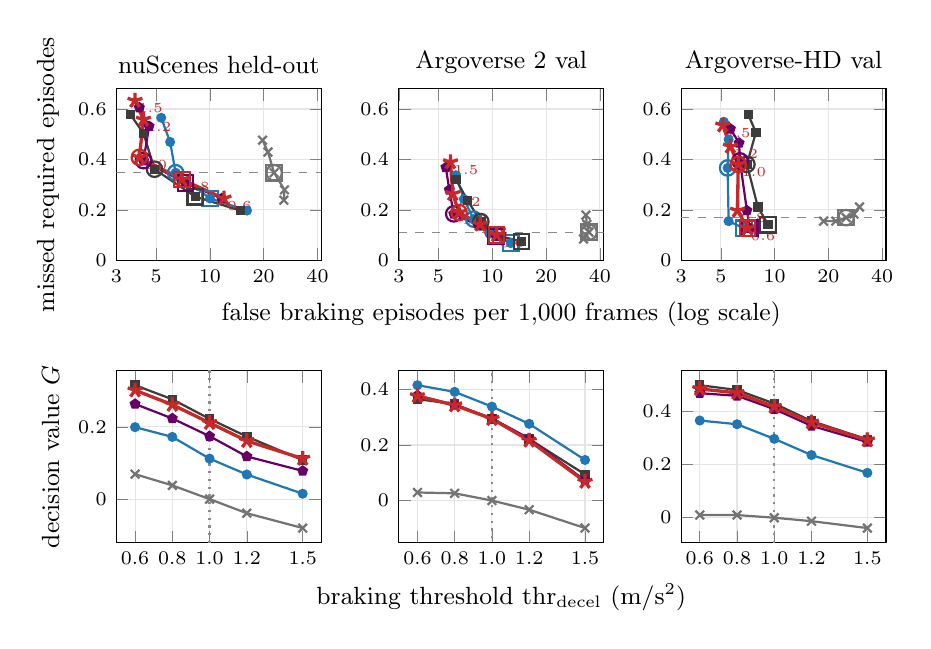
\begin{tikzpicture}
\begin{groupplot}[group style={group size=3 by 2, horizontal sep=28pt, vertical sep=40pt},
  width=0.345\linewidth, height=0.31\linewidth, tick label style={font=\scriptsize},
  label style={font=\small}, title style={font=\small, yshift=-4pt}, grid=major, grid style={gray!20},
  yticklabel style={/pgf/number format/fixed, /pgf/number format/precision=2},
  legend style={font=\scriptsize, draw=gray!50, column sep=4pt}, legend cell align=left]
\nextgroupplot[title={nuScenes held-out}, xmode=log, xmin=3, xmax=42, xtick={3,5,10,20,40}, xticklabels={3,5,10,20,40}, ymin=0, ymax=0.68, ylabel={missed required episodes}, legend to name=oclegend, legend columns=5]
\draw[black!45, dashed] (axis cs:3,0.347) -- (axis cs:42,0.347);
\addplot[black!55, thick, mark=x, mark size=2.2pt] coordinates {(25.92,0.238) (26.14,0.279) (22.87,0.347) (21.13,0.429) (19.71,0.476)};
\addlegendentry{Cheap (u320)}
\addplot[black!55, only marks, mark=o, mark size=2.8pt, thick, forget plot] coordinates {(22.87,0.347)};
\addplot[black!55, only marks, mark=square, mark size=2.8pt, thick, forget plot] coordinates {(22.87,0.347)};
\addplot[adac, thick, mark=*, mark size=1.4pt] coordinates {(16.12,0.197) (10.02,0.245) (6.43,0.347) (5.99,0.469) (5.34,0.565)};
\addlegendentry{u960 + comp.}
\addplot[adac, only marks, mark=o, mark size=2.8pt, thick, forget plot] coordinates {(6.43,0.347)};
\addplot[adac, only marks, mark=square, mark size=2.8pt, thick, forget plot] coordinates {(10.02,0.245)};
\addplot[unic, thick, mark=square*, mark size=1.3pt] coordinates {(14.81,0.197) (8.28,0.252) (4.90,0.361) (4.25,0.503) (3.59,0.578)};
\addlegendentry{Native + comp.}
\addplot[unic, only marks, mark=o, mark size=2.8pt, thick, forget plot] coordinates {(4.90,0.361)};
\addplot[unic, only marks, mark=square, mark size=2.8pt, thick, forget plot] coordinates {(8.28,0.252)};
\addplot[violet!80!black, thick, mark=pentagon*, mark size=1.6pt] coordinates {(11.65,0.245) (7.30,0.306) (4.25,0.395) (4.57,0.531) (4.03,0.605)};
\addlegendentry{Support + corridor tube}
\addplot[violet!80!black, only marks, mark=o, mark size=2.8pt, thick, forget plot] coordinates {(4.25,0.395)};
\addplot[violet!80!black, only marks, mark=square, mark size=2.8pt, thick, forget plot] coordinates {(7.30,0.306)};
\addplot[oursc, very thick, mark=star, mark size=2.8pt] coordinates {(11.98,0.245) (6.97,0.320) (4.03,0.408) (4.25,0.558) (3.81,0.633)};
\addlegendentry{\method}
\addplot[oursc, only marks, mark=o, mark size=2.8pt, thick, forget plot] coordinates {(4.03,0.408)};
\addplot[oursc, only marks, mark=square, mark size=2.8pt, thick, forget plot] coordinates {(6.97,0.320)};
\node[font=\tiny, text=oursc, anchor=north west, inner sep=1pt] at (axis cs:11.98,0.245) {0.6};
\node[font=\tiny, text=oursc, anchor=north west, inner sep=1pt] at (axis cs:6.97,0.320) {0.8};
\node[font=\tiny, text=oursc, anchor=north west, inner sep=1pt] at (axis cs:4.03,0.408) {1.0};
\node[font=\tiny, text=oursc, anchor=north west, inner sep=1pt] at (axis cs:4.25,0.558) {1.2};
\node[font=\tiny, text=oursc, anchor=north west, inner sep=1pt] at (axis cs:3.81,0.633) {1.5};
\nextgroupplot[title={Argoverse~2 val}, xmode=log, xmin=3, xmax=42, xtick={3,5,10,20,40}, xticklabels={3,5,10,20,40}, ymin=0, ymax=0.68, xlabel={false braking episodes per 1{,}000 frames (log scale)}]
\draw[black!45, dashed] (axis cs:3,0.111) -- (axis cs:42,0.111);
\addplot[black!55, thick, mark=x, mark size=2.2pt] coordinates {(32.41,0.084) (33.25,0.100) (34.78,0.111) (33.85,0.142) (33.42,0.179)};
\addplot[black!55, only marks, mark=o, mark size=2.8pt, thick, forget plot] coordinates {(34.78,0.111)};
\addplot[black!55, only marks, mark=square, mark size=2.8pt, thick, forget plot] coordinates {(34.78,0.111)};
\addplot[adac, thick, mark=*, mark size=1.4pt] coordinates {(12.69,0.068) (9.65,0.105) (7.87,0.163) (6.94,0.242) (6.26,0.337)};
\addplot[adac, only marks, mark=o, mark size=2.8pt, thick, forget plot] coordinates {(7.87,0.163)};
\addplot[adac, only marks, mark=square, mark size=2.8pt, thick, forget plot] coordinates {(12.69,0.068)};
\addplot[unic, thick, mark=square*, mark size=1.3pt] coordinates {(14.55,0.074) (11.17,0.095) (8.63,0.153) (7.28,0.237) (6.26,0.321)};
\addplot[unic, only marks, mark=o, mark size=2.8pt, thick, forget plot] coordinates {(8.63,0.153)};
\addplot[unic, only marks, mark=square, mark size=2.8pt, thick, forget plot] coordinates {(14.55,0.074)};
\addplot[violet!80!black, thick, mark=pentagon*, mark size=1.6pt] coordinates {(10.49,0.095) (8.38,0.137) (6.09,0.184) (5.75,0.279) (5.50,0.368)};
\addplot[violet!80!black, only marks, mark=o, mark size=2.8pt, thick, forget plot] coordinates {(6.09,0.184)};
\addplot[violet!80!black, only marks, mark=square, mark size=2.8pt, thick, forget plot] coordinates {(10.49,0.095)};
\addplot[oursc, very thick, mark=star, mark size=2.8pt] coordinates {(10.58,0.100) (8.55,0.142) (6.52,0.189) (6.01,0.263) (5.84,0.389)};
\addplot[oursc, only marks, mark=o, mark size=2.8pt, thick, forget plot] coordinates {(6.52,0.189)};
\addplot[oursc, only marks, mark=square, mark size=2.8pt, thick, forget plot] coordinates {(10.58,0.100)};
\node[font=\tiny, text=oursc, anchor=north west, inner sep=1pt] at (axis cs:10.58,0.100) {0.6};
\node[font=\tiny, text=oursc, anchor=north west, inner sep=1pt] at (axis cs:8.55,0.142) {0.8};
\node[font=\tiny, text=oursc, anchor=north west, inner sep=1pt] at (axis cs:6.52,0.189) {1.0};
\node[font=\tiny, text=oursc, anchor=north west, inner sep=1pt] at (axis cs:6.01,0.263) {1.2};
\node[font=\tiny, text=oursc, anchor=north west, inner sep=1pt] at (axis cs:5.84,0.389) {1.5};
\nextgroupplot[title={Argoverse-HD val}, xmode=log, xmin=3, xmax=42, xtick={3,5,10,20,40}, xticklabels={3,5,10,20,40}, ymin=0, ymax=0.68]
\draw[black!45, dashed] (axis cs:3,0.169) -- (axis cs:42,0.169);
\addplot[black!55, thick, mark=x, mark size=2.2pt] coordinates {(18.79,0.155) (21.99,0.155) (25.12,0.169) (27.79,0.183) (29.85,0.211)};
\addplot[black!55, only marks, mark=o, mark size=2.8pt, thick, forget plot] coordinates {(25.12,0.169)};
\addplot[black!55, only marks, mark=square, mark size=2.8pt, thick, forget plot] coordinates {(25.12,0.169)};
\addplot[adac, thick, mark=*, mark size=1.4pt] coordinates {(6.73,0.127) (5.53,0.155) (5.46,0.366) (5.53,0.479) (5.20,0.549)};
\addplot[adac, only marks, mark=o, mark size=2.8pt, thick, forget plot] coordinates {(5.46,0.366)};
\addplot[adac, only marks, mark=square, mark size=2.8pt, thick, forget plot] coordinates {(6.73,0.127)};
\addplot[unic, thick, mark=square*, mark size=1.3pt] coordinates {(9.20,0.141) (8.06,0.211) (7.00,0.380) (7.86,0.507) (7.13,0.577)};
\addplot[unic, only marks, mark=o, mark size=2.8pt, thick, forget plot] coordinates {(7.00,0.380)};
\addplot[unic, only marks, mark=square, mark size=2.8pt, thick, forget plot] coordinates {(9.20,0.141)};
\addplot[violet!80!black, thick, mark=pentagon*, mark size=1.6pt] coordinates {(7.26,0.127) (7.00,0.197) (6.40,0.394) (6.33,0.465) (5.66,0.521)};
\addplot[violet!80!black, only marks, mark=o, mark size=2.8pt, thick, forget plot] coordinates {(6.40,0.394)};
\addplot[violet!80!black, only marks, mark=square, mark size=2.8pt, thick, forget plot] coordinates {(7.26,0.127)};
\addplot[oursc, very thick, mark=star, mark size=2.8pt] coordinates {(7.06,0.127) (6.20,0.197) (6.26,0.380) (5.66,0.451) (5.13,0.535)};
\addplot[oursc, only marks, mark=o, mark size=2.8pt, thick, forget plot] coordinates {(6.26,0.380)};
\addplot[oursc, only marks, mark=square, mark size=2.8pt, thick, forget plot] coordinates {(7.06,0.127)};
\node[font=\tiny, text=oursc, anchor=north west, inner sep=1pt] at (axis cs:7.06,0.127) {0.6};
\node[font=\tiny, text=oursc, anchor=north west, inner sep=1pt] at (axis cs:6.20,0.197) {0.8};
\node[font=\tiny, text=oursc, anchor=north west, inner sep=1pt] at (axis cs:6.26,0.380) {1.0};
\node[font=\tiny, text=oursc, anchor=north west, inner sep=1pt] at (axis cs:5.66,0.451) {1.2};
\node[font=\tiny, text=oursc, anchor=north west, inner sep=1pt] at (axis cs:5.13,0.535) {1.5};
\nextgroupplot[xmin=0.5, xmax=1.6, xtick={0.6,0.8,1.0,1.2,1.5}, xticklabels={0.6,0.8,1.0,1.2,1.5}, ylabel={decision value $\G$}]
\draw[black!45, dotted, thick] (axis cs:1.0,-1) -- (axis cs:1.0,1);
\addplot[black!55, thick, mark=x, mark size=2.2pt] coordinates {(0.6,0.069) (0.8,0.038) (1.0,0.000) (1.2,-0.039) (1.5,-0.080)};
\addplot[adac, thick, mark=*, mark size=1.4pt] coordinates {(0.6,0.199) (0.8,0.172) (1.0,0.112) (1.2,0.068) (1.5,0.015)};
\addplot[unic, thick, mark=square*, mark size=1.3pt] coordinates {(0.6,0.315) (0.8,0.276) (1.0,0.222) (1.2,0.173) (1.5,0.108)};
\addplot[violet!80!black, thick, mark=pentagon*, mark size=1.6pt] coordinates {(0.6,0.263) (0.8,0.223) (1.0,0.174) (1.2,0.118) (1.5,0.078)};
\addplot[oursc, very thick, mark=star, mark size=2.8pt] coordinates {(0.6,0.301) (0.8,0.261) (1.0,0.211) (1.2,0.161) (1.5,0.112)};
\nextgroupplot[xmin=0.5, xmax=1.6, xtick={0.6,0.8,1.0,1.2,1.5}, xticklabels={0.6,0.8,1.0,1.2,1.5}, xlabel={braking threshold thr$_{\mathrm{decel}}$ (m/s$^2$)}]
\draw[black!45, dotted, thick] (axis cs:1.0,-1) -- (axis cs:1.0,1);
\addplot[black!55, thick, mark=x, mark size=2.2pt] coordinates {(0.6,0.029) (0.8,0.026) (1.0,0.000) (1.2,-0.033) (1.5,-0.099)};
\addplot[adac, thick, mark=*, mark size=1.4pt] coordinates {(0.6,0.415) (0.8,0.391) (1.0,0.338) (1.2,0.276) (1.5,0.146)};
\addplot[unic, thick, mark=square*, mark size=1.3pt] coordinates {(0.6,0.365) (0.8,0.347) (1.0,0.294) (1.2,0.221) (1.5,0.094)};
\addplot[violet!80!black, thick, mark=pentagon*, mark size=1.6pt] coordinates {(0.6,0.378) (0.8,0.344) (1.0,0.296) (1.2,0.223) (1.5,0.072)};
\addplot[oursc, very thick, mark=star, mark size=2.8pt] coordinates {(0.6,0.376) (0.8,0.343) (1.0,0.294) (1.2,0.216) (1.5,0.068)};
\nextgroupplot[xmin=0.5, xmax=1.6, xtick={0.6,0.8,1.0,1.2,1.5}, xticklabels={0.6,0.8,1.0,1.2,1.5}]
\draw[black!45, dotted, thick] (axis cs:1.0,-1) -- (axis cs:1.0,1);
\addplot[black!55, thick, mark=x, mark size=2.2pt] coordinates {(0.6,0.010) (0.8,0.010) (1.0,0.000) (1.2,-0.013) (1.5,-0.039)};
\addplot[adac, thick, mark=*, mark size=1.4pt] coordinates {(0.6,0.366) (0.8,0.352) (1.0,0.297) (1.2,0.236) (1.5,0.169)};
\addplot[unic, thick, mark=square*, mark size=1.3pt] coordinates {(0.6,0.499) (0.8,0.481) (1.0,0.430) (1.2,0.364) (1.5,0.295)};
\addplot[violet!80!black, thick, mark=pentagon*, mark size=1.6pt] coordinates {(0.6,0.469) (0.8,0.459) (1.0,0.409) (1.2,0.346) (1.5,0.285)};
\addplot[oursc, very thick, mark=star, mark size=2.8pt] coordinates {(0.6,0.485) (0.8,0.470) (1.0,0.418) (1.2,0.359) (1.5,0.292)};
\end{groupplot}
\end{tikzpicture}

\vspace{2pt}
\pgfplotslegendfromname{oclegend}
\caption{\textbf{Is the advantage of \method an artifact of its operating point?} Operating curves on the test splits, obtained by varying the braking threshold thr$_{\mathrm{decel}}\in\{0.6,0.8,1.0,1.2,1.5\}$\,m/s$^2$ of the planner (labels at the points of \method); the required episodes and the loss of $\G$ remain those of the deployed planner. Top: share of required braking episodes that are missed \vs false braking episodes per $1{,}000$ frames. Circles: deployed threshold ($1.0$); squares: threshold chosen on development data by the constrained rule of \cref{tab:constrained}; dashed line: missed share of the cheap detector at the deployed threshold. Bottom: decision value \vs threshold. All pipelines except the cheap one use the shared components, and the hybrid receives the per-frame budget of \method at each threshold. Values in \cref{tab:curves}; false-episode rates from the same runs.}
\label{fig:operating}
\end{figure}

% --- Table: constrained operating points (handoff/K37/K37-1: k1_constrained.csv; protocol K37-1/PREREG.md) ---
\begin{table}[!tbp]
\centering
\caption{\textbf{Thresholds selected on development data under a missed-braking criterion.} For each pipeline, the braking threshold thr$_{\mathrm{decel}}$ (m/s$^2$) is the largest value of $\{0.6, 0.8, 1.0, 1.2, 1.5\}$ at which it misses no more required episodes than the cheap detector on the development data (chosen once, before the evaluation; Argoverse-HD uses the Argoverse~2 choice). $^{\S}$: no grid value meets the constraint on the development data (\method misses $31$ \vs $30$ of $366$ episodes); its lowest-miss value is used. Missed: required episodes without braking; False: false braking episodes per $1{,}000$ frames; $\Delta\G$: $95\%$ paired interval of (\method$\,-\,$row), bold if above zero; px in \% of the native frame. The required episodes and the loss of $\G$ remain those of the deployed planner.}
\label{tab:constrained}
\small
\setlength{\tabcolsep}{4pt}
\begin{tabular}{@{}lcccccc@{}}
\toprule
Pipeline & thr$_{\mathrm{decel}}$ & Missed & False & $\G$ & $\Delta\G$ & px \\
\midrule
\multicolumn{7}{@{}l}{\emph{nuScenes held-out}} \\
Cheap (u320) & 1.0 & 51/147 & 22.9 & 0.000 & \best{\ci{+0.145}{+0.396}} & 4.3 \\
u960 + comp. & 0.8 & 36/147 & 10.0 & 0.172 & \ci{$-$0.087}{+0.301} & 38.4 \\
Native + comp. & 0.8 & 37/147 & 8.3 & 0.276 & \ci{$-$0.091}{+0.115} & 103.1 \\
Support + corridor tube & 0.8 & 45/147 & 7.3 & 0.223 & \ci{$-$0.009}{+0.097} & 11.3 \\
\oursrow \textbf{\method} & 0.8 & 47/147 & 7.0 & 0.261 & \na & 8.0 \\
\midrule
\multicolumn{7}{@{}l}{\emph{Argoverse~2 val}} \\
Cheap (u320) & 1.0 & 21/190 & 34.8 & 0.000 & \best{\ci{+0.316}{+0.435}} & 2.6 \\
u960 + comp. & 0.6 & 13/190 & 12.7 & 0.415 & \ci{$-$0.088}{+0.002} & 23.2 \\
Native + comp. & 0.6 & 14/190 & 14.6 & 0.365 & \ci{$-$0.068}{+0.095} & 101.2 \\
Support + corridor tube & 0.6 & 18/190 & 10.5 & 0.378 & \ci{$-$0.013}{+0.009} & 7.8 \\
\oursrow \textbf{\method} & 0.6$^{\S}$ & 19/190 & 10.6 & 0.376 & \na & 5.7 \\
\midrule
\multicolumn{7}{@{}l}{\emph{Argoverse-HD val}} \\
Cheap (u320) & 1.0 & 12/71 & 25.1 & 0.000 & \best{\ci{+0.375}{+0.584}} & 3.1 \\
u960 + comp. & 0.6 & 9/71 & 6.7 & 0.366 & \best{\ci{+0.016}{+0.311}} & 25.3 \\
Native + comp. & 0.6 & 10/71 & 9.2 & 0.499 & \ci{$-$0.047}{+0.022} & 101.3 \\
Support + corridor tube & 0.6 & 9/71 & 7.3 & 0.469 & \best{\ci{+0.006}{+0.030}} & 11.2 \\
\oursrow \textbf{\method} & 0.6$^{\S}$ & 9/71 & 7.1 & 0.485 & \na & 7.3 \\
\midrule
\multicolumn{7}{@{}l}{\emph{Held-out sequences}} \\
Cheap (u320) & 1.0 & 18/154 & 34.5 & 0.000 & \best{\ci{+0.412}{+0.529}} & 3.1 \\
u960 + comp. & 0.6 & 20/154 & 8.0 & 0.457 & \best{\ci{+0.002}{+0.027}} & 25.3 \\
Native + comp. & 0.6 & 19/154 & 9.5 & 0.483 & \ci{$-$0.023}{+0.006} & 101.3 \\
Support + corridor tube & 0.6 & 24/154 & 8.6 & 0.474 & \ci{$-$0.011}{+0.008} & 13.4 \\
\oursrow \textbf{\method} & 0.6$^{\S}$ & 20/154 & 7.1 & 0.474 & \na & 7.9 \\
\bottomrule
\end{tabular}
\end{table}

\Cref{tab:curves} sweeps the braking threshold of the planner for \method, the hybrid, and whole-frame inference with the same components; the required episodes and the loss of $\G$ remain those of the deployed planner, and the deployed threshold reproduces the stored results exactly.
Lowering the threshold moves every pipeline with the components along the same trade-off: the missed episodes of \method fall from $60$, $36$, and $27$ to $36$, $19$, and $9$ between $1.0$ and $0.6$, its decision value rises, and its false braking episodes rise from $4.0$, $6.5$, and $6.3$ to $12.0$, $10.6$, and $7.1$ per $1{,}000$ frames; at every threshold, \method uses significantly fewer pixels than the hybrid, whose decision value is never significantly higher (on Argoverse~2, it is higher by $0.002$--$0.006$, not significant; on Argoverse-HD, it is significantly lower at $0.6$ and $1.2$).
\Cref{tab:constrained} evaluates once, on the test splits and the held-out sequences, the threshold of each pipeline that a rule fixed in advance selected on the development data.
At this point, \method does not miss significantly more episodes than the cheap detector on any split, brakes falsely $16$--$27$ fewer times per $1{,}000$ frames, and attains a decision value that no pipeline with the same components exceeds significantly; whole-frame inference with the components misses fewer episodes on nuScenes and Argoverse~2 with $3$--$18\times$ the pixels.
The deployed threshold was not changed in response to these results.

\subsection{Held-out sequences}
\label{sec:supp_holdout}

% --- Table: held-out sequences (handoff/K35/K35-4: k4_rows.csv, k4_diffs.csv, k4_episodes.csv; protocol in K35-4/PREREG.md) ---
\begin{table}[!tbp]
\centering
\caption{\textbf{Held-out sequences} ($65$ Argoverse-HD training sequences, $39{,}265$ frames, $154$ required episodes), in the first of two evaluations under protocols fixed in advance. $\Delta\G$: $95\%$ paired interval of (\method$\,-\,$row), bold if above zero. Missed: required braking episodes without braking. ``+ comp.'': with the refiner and the learned looming estimate.}
\label{tab:holdout}
\footnotesize
\setlength{\tabcolsep}{2.2pt}
\begin{tabular}{@{}lccccc@{}}
\toprule
Pipeline & $\G$ & $\Delta\G$ & px\,(\%) & False & Missed \\
\midrule
Cheap (u320) & 0 & \best{\ci{+0.313}{+0.480}} & 3.1 & 34.5 & 18 \\
u960 + comp. & 0.400 & \ci{$-$0.012}{+0.021} & 25.3 & 6.4 & 42 \\
Native + comp. & 0.417 & \ci{$-$0.026}{+0.008} & 101.3 & 8.2 & 44 \\
Support + corridor tube & 0.410 & \ci{$-$0.011}{+0.005} & 12.6 & 7.7 & 44 \\
Uncertainty crops & 0.338 & \best{\ci{+0.046}{+0.093}} & 15.2 & 20.7 & 32 \\
AnA-style, iterated & 0.408 & \ci{$-$0.022}{+0.012} & 12.4 & 7.5 & 44 \\
\midrule
\oursrow \textbf{\method} & 0.407 & \na & 7.6 & 6.5 & 43 \\
Bounded + temporal recovery & 0.409 & \ci{$-$0.011}{+0.002} & 6.9 & 7.6 & 42 \\
\bottomrule
\end{tabular}
\end{table}

The frozen configuration and the baselines of \cref{tab:holdout} were run once on the $65$ training sequences of Argoverse-HD, previously unused for training, configuration selection, and evaluation, with the code, the rows, the metrics, and the decision rule fixed in a protocol before the run; the sequences were used once more, for the constrained operating points of \cref{tab:constrained} under a second protocol, and for no other evaluation or choice.
The sequences share the sensor, the cities, and the annotation process of the Argoverse-HD test split and contain only $17$ episodes that require hard braking.
\method attains $\G=0.407$ with $7.6\%$ of the native pixels; no baseline with the same components differs significantly from it, although they use $1.6$--$13\times$ its pixels, and uncertainty crops are significantly lower.
All pipelines with the same components miss $42$--$44$ of the $154$ required episodes, compared with $18$ for the cheap detector at $34.5$ false braking episodes per $1{,}000$ frames.
The protocol also contained one candidate extension, fixed on development data before the run: bounded-keep (\cref{sec:supp_latency}), together with the recovery of missing looming observations of verified objects from the retained previous frames.
It attains the decision value of \method ($\Delta\G$ in \cref{tab:holdout}) with $10\%$ fewer pixels and $1.0$ more false braking episode per $1{,}000$ frames ($\ci{+0.49}{+1.62}$); it is not used elsewhere in this paper.

\subsection{Stratified evaluation}
\label{sec:supp_strata}

% --- Table: distribution-shift strata (handoff/K31/strata.csv) ---
\begin{table}[!tbp]
\centering
\caption{\textbf{Decision value per stratum} (lighting and rain from the nuScenes scene descriptions; city for Argoverse~2 and Argoverse-HD). All baselines with the shared components. $^{\dagger}$ / $^{\ast}$: \method significantly better / worse within the stratum.}
\label{tab:strata}
\footnotesize
\setlength{\tabcolsep}{2.2pt}
\begin{tabular}{@{}lcccccc@{}}
\toprule
Stratum & Units & u960 & Native & Hybrid & Uncert. & \method \\
\midrule
nuScenes, day & 201 & 0.233 & 0.237 & 0.195 & 0.163$^{\dagger}$ & 0.197 \\
nuScenes, night & 27 & $-$0.061 & 0.201 & 0.144 & $-$0.379$^{\dagger}$ & 0.231 \\
nuScenes, no rain & 178 & $-$0.002 & 0.191 & 0.091 & $-$0.106$^{\dagger}$ & 0.140 \\
nuScenes, rain & 50 & 0.479 & 0.323 & 0.440 & 0.093$^{\dagger}$ & 0.440 \\
\midrule
Argoverse~2, ATX & 4 & 0.272 & 0.298 & 0.186 & 0.199 & 0.191 \\
Argoverse~2, DTW & 21 & 0.461 & 0.197 & 0.473 & 0.185$^{\dagger}$ & 0.491 \\
Argoverse~2, MIA & 49 & 0.303 & 0.222 & 0.225 & 0.160$^{\dagger}$ & 0.223 \\
Argoverse~2, PAO & 7 & 0.481 & 0.504 & 0.412 & 0.377 & 0.442 \\
Argoverse~2, PIT & 51 & 0.292 & 0.327 & 0.321 & 0.237$^{\dagger}$ & 0.309 \\
Argoverse~2, WDC & 18 & 0.456 & 0.468$^{\ast}$ & 0.279 & 0.357 & 0.269 \\
\midrule
Argoverse-HD, MIA & 10 & 0.393 & 0.442 & 0.413 & 0.280$^{\dagger}$ & 0.415 \\
Argoverse-HD, PIT & 14 & 0.174$^{\dagger}$ & 0.415 & 0.402$^{\dagger}$ & 0.284$^{\dagger}$ & 0.421 \\
\bottomrule
\end{tabular}
\end{table}

\method attains a positive decision value in every stratum of \cref{tab:strata}, including the night scenes of nuScenes ($0.231$, compared with $-0.061$ for u960) and rain ($0.440$).
In the $14$ Argoverse-HD sequences of Pittsburgh, \method is significantly better than u960 and the hybrid.
The strata are subsets of the evaluated datasets, not an independent test of domain generalization.

\subsection{Robustness of the evaluation}
\label{sec:supp_robust}

Across $27$ weightings of the loss terms (excessive braking, collisions, and command changes each scaled by $0.5$, $1$, or $2$), \method ranks second of ten pipelines on nuScenes and Argoverse-HD and third or fourth on Argoverse~2, and its decision value is at least $0.166$, $0.159$, and $0.335$ in every setting, including the one in which excessive braking is halved and collisions are doubled, \ie, in which insufficient braking weighs twice as much relative to excessive braking.
With the braking thresholds scaled by $0.8$ or $1.2$ or a reaction time of $0.3$ or $0.6$\,s, which change the field through the planner, \method remains significantly better than uncertainty crops on every dataset and in every tested setting; these checks do not cover every possible loss.


% --- K40-2 (handoff/K40R/k40_2_weights.csv, k40_2_safety_deltas.csv; CPU, from stored actions; pre-specified post-hoc) ---
\subsection{Losses that weight insufficient braking more}
\label{sec:supp_safety}

\begin{table}[!htbp]
\centering
\caption{\textbf{Decision value when insufficient braking weighs more}, with the insufficient-braking term of the loss multiplied by $w$ and all other terms fixed, computed from the stored actions of each pipeline (uncapped). $^{\dagger}$ / $^{\ast}$: \method significantly better / worse ($95\%$ paired interval); $^{\ddagger}$ / $^{\ast\ast}$: also after Holm correction over all compared pipelines and weights of a dataset.}
\label{tab:safety}
\footnotesize
\setlength{\tabcolsep}{1.9pt}
\begin{tabular}{@{}lcccccccccccccc@{}}
\toprule
 & \multicolumn{4}{c}{nuScenes held-out} & & \multicolumn{4}{c}{Argoverse~2 val} & & \multicolumn{4}{c}{Argoverse-HD val} \\
\cmidrule(lr){2-5}\cmidrule(lr){7-10}\cmidrule(l){12-15}
$w$ & $1$ & $2$ & $5$ & $10$ & & $1$ & $2$ & $5$ & $10$ & & $1$ & $2$ & $5$ & $10$ \\
\midrule
u960 + comp. & 0.112 & 0.077 & 0.052 & 0.043 & & 0.338 & 0.239$^{\ast}$ & 0.132$^{\ast}$ & 0.080$^{\ast}$ & & 0.297$^{\dagger}$ & 0.259$^{\dagger}$ & 0.195 & 0.148 \\
u1280 + comp. & 0.292 & 0.269 & 0.251$^{\ast}$ & 0.245$^{\ast}$ & & 0.348$^{\ast}$ & 0.252$^{\ast}$ & 0.148$^{\ast}$ & 0.097$^{\ast}$ & & 0.315$^{\dagger}$ & 0.279$^{\dagger}$ & 0.218 & 0.174 \\
Native + comp. & 0.222 & 0.175 & 0.140 & 0.128 & & 0.294 & 0.160 & 0.015 & $-$0.054 & & 0.430 & 0.369 & 0.265 & 0.189 \\
AdaScale & 0.144 & 0.113 & 0.091 & 0.083 & & 0.341 & 0.244$^{\ast}$ & 0.139$^{\ast}$ & 0.088$^{\ast}$ & & 0.298$^{\ddagger}$ & 0.261$^{\dagger}$ & 0.198 & 0.152 \\
SAHI & 0.303 & 0.309$^{\ast}$ & 0.314$^{\ast\ast}$ & 0.315$^{\ast\ast}$ & & 0.256 & 0.210 & 0.160$^{\ast}$ & 0.135$^{\ast\ast}$ & & 0.229$^{\ddagger}$ & 0.231$^{\dagger}$ & 0.234 & 0.236 \\
AnA-style, iterated & 0.158 & 0.117 & 0.088 & 0.077 & & 0.349$^{\ast}$ & 0.241$^{\ast}$ & 0.125$^{\ast}$ & 0.068$^{\ast}$ & & 0.315$^{\dagger}$ & 0.268$^{\dagger}$ & 0.188$^{\dagger}$ & 0.130 \\
Support + tube & 0.174 & 0.129 & 0.096 & 0.083 & & 0.296 & 0.170 & 0.033 & $-$0.033 & & 0.408 & 0.346 & 0.242 & 0.166 \\
Reference $\policy(\full)$ & 0.085 & 0.049 & 0.023 & 0.013 & & 0.290 & 0.256$^{\ast}$ & 0.219$^{\ast\ast}$ & 0.201$^{\ast\ast}$ & & 0.296 & 0.322 & 0.367 & 0.400$^{\ast}$ \\
\method w/o refiner & 0.181 & 0.131$^{\dagger}$ & 0.094$^{\dagger}$ & 0.081$^{\dagger}$ & & 0.241$^{\dagger}$ & 0.169 & 0.091 & 0.053$^{\ast}$ & & 0.422 & 0.422 & 0.423$^{\ast}$ & 0.423$^{\ast\ast}$ \\
\oursrow \textbf{\method} & \textbf{0.211} & \textbf{0.166} & \textbf{0.134} & \textbf{0.122} & & \textbf{0.294} & \textbf{0.166} & \textbf{0.027} & \textbf{$-$0.039} & & \textbf{0.418} & \textbf{0.357} & \textbf{0.254} & \textbf{0.179} \\
\bottomrule
\end{tabular}
\end{table}

The weightings of \cref{sec:supp_robust} scale the excessive-braking, collision, and command-change terms.
\Cref{tab:safety} instead multiplies the insufficient-braking term by $2$, $5$, and $10$.
Since most of the gain of \method comes from fewer excessive braking actions (\cref{sec:supp_composition}), its decision value falls with this weight, to $0.122$, $-0.039$, and $0.179$ at $w=10$, where it no longer differs significantly from that of the cheap pipeline on any dataset.
On nuScenes, only SAHI (from $w=2$) and whole-frame inference at $1280$ pixels (from $w=5$) score significantly higher, and on Argoverse-HD, no compared method does at any weight.
On Argoverse~2, whole-frame inference at $960$ and $1280$ pixels, AdaScale, AnA-style refinement, and SAHI score significantly higher from $w=2$ or $5$, after Holm correction only SAHI at $w=10$.
The range refiner accounts for much of this decline on Argoverse~2 and Argoverse-HD: without it, \method keeps $\G=0.42$ on Argoverse-HD at every weight and attains $0.053$ on Argoverse~2 at $w=10$, and the reference without the refiner attains $0.201$ and $0.400$; on nuScenes, the refiner raises the decision value at every weight.
The refiner thus trades insufficient for excessive braking, and the decision value under the deployed weights is not a measure of safety.

%%%%%%%%%%%%%%%%%%%%%%%%%%%%%%%%%%%%%%%%%%%%%%%%%%%%%%%%%%%%%%%%%%%%%%%%%%%%%%
%% S6. EMBEDDED LATENCY, DEADLINES, CLOSED LOOP, PLANNING
%%%%%%%%%%%%%%%%%%%%%%%%%%%%%%%%%%%%%%%%%%%%%%%%%%%%%%%%%%%%%%%%%%%%%%%%%%%%%%
\section{Embedded latency, deadlines, closed loop, and planning}
\label{sec:supp_embedded}

This section reports the latency and energy of \method and of all compared methods on a Jetson AGX Xavier (\cref{sec:supp_latency}), the decision value under per-frame deadlines run on the device (\cref{sec:supp_deadline}), the controlled closed loop in CARLA (\cref{sec:supp_aeb}), and the planning benchmarks (\cref{sec:supp_planning}).

\subsection{Latency and energy}
\label{sec:supp_latency}

% --- Table: latency (handoff/K29/latency_fast.csv, path trt32, 3 repetitions at MAXN; G on the timed frames) ---
\begin{table}[!tbp]
\centering
\caption{\textbf{Latency on a Jetson AGX Xavier} (ms). \method is $1.7$--$1.8\times$ faster than native-resolution inference with the same components. $\G$ on the timed frames ($805$ frames of $20$ nuScenes held-out scenes; $586$ frames of $8$ Argoverse~2 logs). Bounded-drop: at most two crop batches, pending truncated detections discarded (\cref{sec:supp_latency}).}
\label{tab:latency}
\small
\setlength{\tabcolsep}{2.6pt}
\begin{tabular}{@{}lgccgcc@{}}
\toprule
 & \multicolumn{3}{c}{nuScenes} & \multicolumn{3}{c}{Argoverse 2} \\
\cmidrule(lr){2-4}\cmidrule(l){5-7}
Pipeline & $\G\uparrow$ & Mean & p95 & $\G\uparrow$ & Mean & p95 \\
\midrule
Cheap (u320) & 0 & 7.5 & 8.2 & 0 & 10.4 & 10.9 \\
u512 + comp. & 0.336 & 13.9 & 22.1 & 0.363 & 24.3 & 39.7 \\
u960 + comp. & 0.386 & 22.7 & 30.9 & 0.323 & 34.3 & 49.2 \\
u1280 + comp. & 0.395 & 28.6 & 36.5 & 0.311 & 43.6 & 59.3 \\
Native + comp. & 0.364 & 37.9 & 45.5 & 0.410 & 75.7 & 88.7 \\
\midrule
\oursrow \textbf{\method} & 0.380 & 21.9 & 59.2 & 0.419 & 41.7 & 93.8 \\
\oursrow \textbf{\method}, bounded-drop & 0.382 & 19.8 & 46.2 & 0.423 & 37.1 & 73.5 \\
\bottomrule
\end{tabular}
\end{table}

The detectors run as TensorRT FP16 engines at maximum clocks; image decoding is excluded, the first 200 frames serve as warm-up, and all pipelines are timed on the same frames.
The looming estimate encodes all crops of a lift step in one batched TensorRT call, caches the feature of each crop for the two following frames, and skips the objects whose demand cannot depend on their time-to-collision, \ie, objects outside the ego corridor or beyond $80$\,m; the 64$\times$64 crops are shared with the refiner.
On the full development splits, these changes leave every action of every pipeline unchanged.
The tail of the latency of the unbounded loop stems from the detector calls of the truncation guard, not from the looming estimate.
We therefore evaluate two variants that return the action of the merged scene after at most two crop batches after the draft; each batch processes the new crops of the field and the support together with the enlarged crops that the guard has queued in the previous batch, and a batch can be split into several executions of the detector engine.
\emph{Bounded-drop} discards the detections whose guard re-detection is still pending at the bound; \emph{bounded-keep}, selected on the development data, keeps them as detected.
The deadline experiments (\cref{fig:deadline}, \cref{tab:deadline,tab:frontier}) and the held-out extension (\cref{sec:supp_holdout}) use bounded-keep; \cref{tab:latency}, the single run from which main \mref{tab:eff} takes its latencies, reports bounded-drop.
\begin{itemize}[leftmargin=12pt, itemsep=1pt, topsep=2pt]
\item \emph{Bounded-drop} exceeds $50$, $66.7$, and $100$\,ms on $3.1\%$, $0.2\%$, and none of the timed nuScenes frames, compared with $9.4\%$, $2.7\%$, and $0.2\%$ for \method and $0.5\%$ and $1.2\%$ above $50$\,ms and none above $66.7$\,ms for u960 and native-resolution inference with the components; on the full test splits, however, it attains $\G=0.091$, $0.282$, and $0.419$, the loss on nuScenes stemming from one scene.
\item \emph{Bounded-keep} attains $\G=0.209$, $0.293$, and $0.415$ on the full test splits with $6$--$10\%$ fewer pixels than \method, within $\ci{-0.005}{+0.002}$, $\ci{-0.007}{+0.005}$, and $\ci{-0.008}{+0.001}$ of \method. Timed in separate runs on the same frames, it runs at $20.3$ and $38.5$\,ms on average on nuScenes and Argoverse~2, with a $95$th percentile of $49.1$ and $77.4$\,ms, compared with $21.8$ and $40.4$\,ms and $59.7$ and $91.2$\,ms for \method (paired differences of the $95$th percentile $\ci{-14.7}{-2.5}$ and $\ci{-22.8}{-6.4}$\,ms); it exceeds $100$\,ms on none and $1.1\%$ of the frames.
\end{itemize}

\begin{figure}[!htbp]
\centering
% plot generated from the reference tables (script: versions/paper_tools_2026-10-27/make_supp_figs.py)
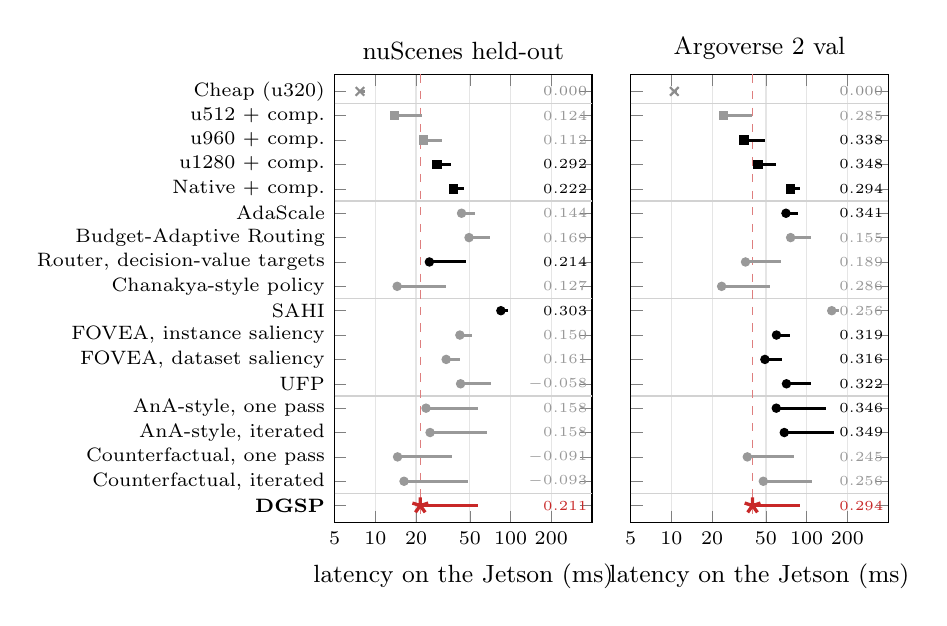
\begin{tikzpicture}
\begin{groupplot}[group style={group size=2 by 1, horizontal sep=14pt, yticklabels at=edge left},
  width=0.40\linewidth, height=0.60\linewidth, xmode=log, xmin=5, xmax=400,
  xtick={5,10,20,50,100,200}, xticklabels={5,10,20,50,100,200},
  ymin=-0.7, ymax=17.7, ytick={0,...,17}, y dir=reverse,
  yticklabels={{Cheap (u320)},{u512 + comp.},{u960 + comp.},{u1280 + comp.},{Native + comp.},{AdaScale},{Budget-Adaptive Routing},{Router, decision-value targets},{Chanakya-style policy},{SAHI},{FOVEA, instance saliency},{FOVEA, dataset saliency},{UFP},{AnA-style, one pass},{AnA-style, iterated},{Counterfactual, one pass},{Counterfactual, iterated},{\textbf{\method}}},
  tick label style={font=\scriptsize}, label style={font=\small}, title style={font=\small, yshift=-4pt},
  xmajorgrids, grid style={gray!20}, xlabel={latency on the Jetson (ms)}]
\nextgroupplot[title={nuScenes held-out}]
\draw[gray!35] (axis cs:5,0.5) -- (axis cs:400,0.5);
\draw[gray!35] (axis cs:5,4.5) -- (axis cs:400,4.5);
\draw[gray!35] (axis cs:5,8.5) -- (axis cs:400,8.5);
\draw[gray!35] (axis cs:5,12.5) -- (axis cs:400,12.5);
\draw[gray!35] (axis cs:5,16.5) -- (axis cs:400,16.5);
\draw[oursc!60, dashed] (axis cs:21.5,-0.7) -- (axis cs:21.5,17.7);
\draw[black!45, line width=1.1pt] (axis cs:7.7,0) -- (axis cs:8.4,0);
\addplot[black!45, only marks, mark=x, mark size=2.2pt, thick] coordinates {(7.7,0)};
\node[font=\tiny, text=black!45, anchor=east, inner sep=1pt] at (axis cs:390,0) {$0.000$};
\draw[black!40, line width=1.1pt] (axis cs:13.9,1) -- (axis cs:22.1,1);
\addplot[black!40, only marks, mark=square*, mark size=1.5pt] coordinates {(13.9,1)};
\node[font=\tiny, text=black!40, anchor=east, inner sep=1pt] at (axis cs:390,1) {$0.124$};
\draw[black!40, line width=1.1pt] (axis cs:22.7,2) -- (axis cs:30.9,2);
\addplot[black!40, only marks, mark=square*, mark size=1.5pt] coordinates {(22.7,2)};
\node[font=\tiny, text=black!40, anchor=east, inner sep=1pt] at (axis cs:390,2) {$0.112$};
\draw[black, line width=1.1pt] (axis cs:28.6,3) -- (axis cs:36.5,3);
\addplot[black, only marks, mark=square*, mark size=1.5pt] coordinates {(28.6,3)};
\node[font=\tiny, text=black, anchor=east, inner sep=1pt] at (axis cs:390,3) {$0.292$};
\draw[black, line width=1.1pt] (axis cs:37.9,4) -- (axis cs:45.5,4);
\addplot[black, only marks, mark=square*, mark size=1.5pt] coordinates {(37.9,4)};
\node[font=\tiny, text=black, anchor=east, inner sep=1pt] at (axis cs:390,4) {$0.222$};
\draw[black!40, line width=1.1pt] (axis cs:43.4,5) -- (axis cs:54.5,5);
\addplot[black!40, only marks, mark=*, mark size=1.5pt] coordinates {(43.4,5)};
\node[font=\tiny, text=black!40, anchor=east, inner sep=1pt] at (axis cs:390,5) {$0.144$};
\draw[black!40, line width=1.1pt] (axis cs:49.3,6) -- (axis cs:70.3,6);
\addplot[black!40, only marks, mark=*, mark size=1.5pt] coordinates {(49.3,6)};
\node[font=\tiny, text=black!40, anchor=east, inner sep=1pt] at (axis cs:390,6) {$0.169$};
\draw[black, line width=1.1pt] (axis cs:25.1,7) -- (axis cs:46.9,7);
\addplot[black, only marks, mark=*, mark size=1.5pt] coordinates {(25.1,7)};
\node[font=\tiny, text=black, anchor=east, inner sep=1pt] at (axis cs:390,7) {$0.214$};
\draw[black!40, line width=1.1pt] (axis cs:14.5,8) -- (axis cs:33.1,8);
\addplot[black!40, only marks, mark=*, mark size=1.5pt] coordinates {(14.5,8)};
\node[font=\tiny, text=black!40, anchor=east, inner sep=1pt] at (axis cs:390,8) {$0.127$};
\draw[black, line width=1.1pt] (axis cs:84.8,9) -- (axis cs:96.0,9);
\addplot[black, only marks, mark=*, mark size=1.5pt] coordinates {(84.8,9)};
\node[font=\tiny, text=black, anchor=east, inner sep=1pt] at (axis cs:390,9) {$0.303$};
\draw[black!40, line width=1.1pt] (axis cs:42.2,10) -- (axis cs:51.7,10);
\addplot[black!40, only marks, mark=*, mark size=1.5pt] coordinates {(42.2,10)};
\node[font=\tiny, text=black!40, anchor=east, inner sep=1pt] at (axis cs:390,10) {$0.150$};
\draw[black!40, line width=1.1pt] (axis cs:33.4,11) -- (axis cs:42.0,11);
\addplot[black!40, only marks, mark=*, mark size=1.5pt] coordinates {(33.4,11)};
\node[font=\tiny, text=black!40, anchor=east, inner sep=1pt] at (axis cs:390,11) {$0.161$};
\draw[black!40, line width=1.1pt] (axis cs:42.7,12) -- (axis cs:71.9,12);
\addplot[black!40, only marks, mark=*, mark size=1.5pt] coordinates {(42.7,12)};
\node[font=\tiny, text=black!40, anchor=east, inner sep=1pt] at (axis cs:390,12) {$-0.058$};
\draw[black!40, line width=1.1pt] (axis cs:23.7,13) -- (axis cs:57.8,13);
\addplot[black!40, only marks, mark=*, mark size=1.5pt] coordinates {(23.7,13)};
\node[font=\tiny, text=black!40, anchor=east, inner sep=1pt] at (axis cs:390,13) {$0.158$};
\draw[black!40, line width=1.1pt] (axis cs:25.4,14) -- (axis cs:66.9,14);
\addplot[black!40, only marks, mark=*, mark size=1.5pt] coordinates {(25.4,14)};
\node[font=\tiny, text=black!40, anchor=east, inner sep=1pt] at (axis cs:390,14) {$0.158$};
\draw[black!40, line width=1.1pt] (axis cs:14.6,15) -- (axis cs:36.9,15);
\addplot[black!40, only marks, mark=*, mark size=1.5pt] coordinates {(14.6,15)};
\node[font=\tiny, text=black!40, anchor=east, inner sep=1pt] at (axis cs:390,15) {$-0.091$};
\draw[black!40, line width=1.1pt] (axis cs:16.3,16) -- (axis cs:48.1,16);
\addplot[black!40, only marks, mark=*, mark size=1.5pt] coordinates {(16.3,16)};
\node[font=\tiny, text=black!40, anchor=east, inner sep=1pt] at (axis cs:390,16) {$-0.093$};
\draw[oursc, line width=1.1pt] (axis cs:21.5,17) -- (axis cs:57.4,17);
\addplot[oursc, only marks, mark=star, mark size=3pt, very thick] coordinates {(21.5,17)};
\node[font=\tiny, text=oursc, anchor=east, inner sep=1pt] at (axis cs:390,17) {$0.211$};
\nextgroupplot[title={Argoverse~2 val}]
\draw[gray!35] (axis cs:5,0.5) -- (axis cs:400,0.5);
\draw[gray!35] (axis cs:5,4.5) -- (axis cs:400,4.5);
\draw[gray!35] (axis cs:5,8.5) -- (axis cs:400,8.5);
\draw[gray!35] (axis cs:5,12.5) -- (axis cs:400,12.5);
\draw[gray!35] (axis cs:5,16.5) -- (axis cs:400,16.5);
\draw[oursc!60, dashed] (axis cs:39.8,-0.7) -- (axis cs:39.8,17.7);
\draw[black!45, line width=1.1pt] (axis cs:10.5,0) -- (axis cs:11.0,0);
\addplot[black!45, only marks, mark=x, mark size=2.2pt, thick] coordinates {(10.5,0)};
\node[font=\tiny, text=black!45, anchor=east, inner sep=1pt] at (axis cs:390,0) {$0.000$};
\draw[black!40, line width=1.1pt] (axis cs:24.3,1) -- (axis cs:39.7,1);
\addplot[black!40, only marks, mark=square*, mark size=1.5pt] coordinates {(24.3,1)};
\node[font=\tiny, text=black!40, anchor=east, inner sep=1pt] at (axis cs:390,1) {$0.285$};
\draw[black, line width=1.1pt] (axis cs:34.3,2) -- (axis cs:49.2,2);
\addplot[black, only marks, mark=square*, mark size=1.5pt] coordinates {(34.3,2)};
\node[font=\tiny, text=black, anchor=east, inner sep=1pt] at (axis cs:390,2) {$0.338$};
\draw[black, line width=1.1pt] (axis cs:43.6,3) -- (axis cs:59.3,3);
\addplot[black, only marks, mark=square*, mark size=1.5pt] coordinates {(43.6,3)};
\node[font=\tiny, text=black, anchor=east, inner sep=1pt] at (axis cs:390,3) {$0.348$};
\draw[black, line width=1.1pt] (axis cs:75.7,4) -- (axis cs:88.7,4);
\addplot[black, only marks, mark=square*, mark size=1.5pt] coordinates {(75.7,4)};
\node[font=\tiny, text=black, anchor=east, inner sep=1pt] at (axis cs:390,4) {$0.294$};
\draw[black, line width=1.1pt] (axis cs:70.3,5) -- (axis cs:86.3,5);
\addplot[black, only marks, mark=*, mark size=1.5pt] coordinates {(70.3,5)};
\node[font=\tiny, text=black, anchor=east, inner sep=1pt] at (axis cs:390,5) {$0.341$};
\draw[black!40, line width=1.1pt] (axis cs:76.1,6) -- (axis cs:106.9,6);
\addplot[black!40, only marks, mark=*, mark size=1.5pt] coordinates {(76.1,6)};
\node[font=\tiny, text=black!40, anchor=east, inner sep=1pt] at (axis cs:390,6) {$0.155$};
\draw[black!40, line width=1.1pt] (axis cs:35.3,7) -- (axis cs:65.0,7);
\addplot[black!40, only marks, mark=*, mark size=1.5pt] coordinates {(35.3,7)};
\node[font=\tiny, text=black!40, anchor=east, inner sep=1pt] at (axis cs:390,7) {$0.189$};
\draw[black!40, line width=1.1pt] (axis cs:23.5,8) -- (axis cs:53.8,8);
\addplot[black!40, only marks, mark=*, mark size=1.5pt] coordinates {(23.5,8)};
\node[font=\tiny, text=black!40, anchor=east, inner sep=1pt] at (axis cs:390,8) {$0.286$};
\draw[black!40, line width=1.1pt] (axis cs:153.2,9) -- (axis cs:172.8,9);
\addplot[black!40, only marks, mark=*, mark size=1.5pt] coordinates {(153.2,9)};
\node[font=\tiny, text=black!40, anchor=east, inner sep=1pt] at (axis cs:390,9) {$0.256$};
\draw[black, line width=1.1pt] (axis cs:59.8,10) -- (axis cs:75.8,10);
\addplot[black, only marks, mark=*, mark size=1.5pt] coordinates {(59.8,10)};
\node[font=\tiny, text=black, anchor=east, inner sep=1pt] at (axis cs:390,10) {$0.319$};
\draw[black, line width=1.1pt] (axis cs:49.1,11) -- (axis cs:65.8,11);
\addplot[black, only marks, mark=*, mark size=1.5pt] coordinates {(49.1,11)};
\node[font=\tiny, text=black, anchor=east, inner sep=1pt] at (axis cs:390,11) {$0.316$};
\draw[black, line width=1.1pt] (axis cs:70.9,12) -- (axis cs:107.8,12);
\addplot[black, only marks, mark=*, mark size=1.5pt] coordinates {(70.9,12)};
\node[font=\tiny, text=black, anchor=east, inner sep=1pt] at (axis cs:390,12) {$0.322$};
\draw[black, line width=1.1pt] (axis cs:59.6,13) -- (axis cs:138.5,13);
\addplot[black, only marks, mark=*, mark size=1.5pt] coordinates {(59.6,13)};
\node[font=\tiny, text=black, anchor=east, inner sep=1pt] at (axis cs:390,13) {$0.346$};
\draw[black, line width=1.1pt] (axis cs:68.3,14) -- (axis cs:159.6,14);
\addplot[black, only marks, mark=*, mark size=1.5pt] coordinates {(68.3,14)};
\node[font=\tiny, text=black, anchor=east, inner sep=1pt] at (axis cs:390,14) {$0.349$};
\draw[black!40, line width=1.1pt] (axis cs:36.4,15) -- (axis cs:81.1,15);
\addplot[black!40, only marks, mark=*, mark size=1.5pt] coordinates {(36.4,15)};
\node[font=\tiny, text=black!40, anchor=east, inner sep=1pt] at (axis cs:390,15) {$0.245$};
\draw[black!40, line width=1.1pt] (axis cs:47.8,16) -- (axis cs:109.3,16);
\addplot[black!40, only marks, mark=*, mark size=1.5pt] coordinates {(47.8,16)};
\node[font=\tiny, text=black!40, anchor=east, inner sep=1pt] at (axis cs:390,16) {$0.256$};
\draw[oursc, line width=1.1pt] (axis cs:39.8,17) -- (axis cs:89.1,17);
\addplot[oursc, only marks, mark=star, mark size=3pt, very thick] coordinates {(39.8,17)};
\node[font=\tiny, text=oursc, anchor=east, inner sep=1pt] at (axis cs:390,17) {$0.294$};
\end{groupplot}
\end{tikzpicture}
\caption{\textbf{Which methods reach the decision value of \method, and at what latency?} Mean latency (marker) and $95$th percentile (end of the bar) on the Jetson AGX Xavier, log scale, with the decision value on the full test split at the right. Black: decision value at least that of \method on the dataset; grey: lower; dashed: mean latency of \method. Rows, from the top: the cheap detector; whole-frame inference with the components (squares; latency from \cref{tab:latency}, separate runs on the same frames; decision value from \cref{tab:uniform}); the methods of \mref{tab:main}, all with the shared components (\cref{tab:latency_baselines}).}
\label{fig:latency}
\end{figure}

\Cref{tab:latency_baselines} times the methods of \cref*{M-tab:main} in separate runs on the same frames: every published, learned, or object-level method that attains at least the decision value of \method takes $25.1$--$84.8$\,ms on average, compared with $21.5$ and $39.8$\,ms for \method in the same runs.
Measured on the module rails and above the cheap detector, \method requires $0.29$ and $0.54$\,J per frame on nuScenes and Argoverse~2, compared with $0.54$ and $0.76$\,J for whole-frame inference at the verification resolution and $1.12$ and $2.39$\,J at the native resolution, both with the same components; whole-frame inference at $512$ pixels requires $0.26$ and $0.42$\,J, less than \method (one run per pipeline).

% --- K41-6 / J02 (handoff/K41/REPORT.md, J04/ breakdown) and LATENCY_OPT JP01/JP03 (handoff/LATENCY_OPT_20261030/REPORT.md, PILOT_REPORT.md, JP03_REPORT.md) ---
\noindent\textbf{Where the tail latency comes from.}
In a separate run with a synchronization after every stage (which adds about $4\%$ to the mean), the mean latency of \method over all frames and over the frames at or above its $95$th percentile is $21.5$ and $70.2$\,ms on nuScenes and $33.3$ and $97.6$\,ms on Argoverse~2.
From all frames to these tail frames, the crop rounds grow from $8.8$ to $45.0$\,ms and from $13.4$ to $55.3$\,ms, and the looming estimate of the crops from $1.4$ to $5.3$\,ms and from $4.0$ to $15.8$\,ms, whereas the draft stays at $7$--$10$\,ms, the refiner below $4$\,ms, and the field, guard, lift, and merge together below $13$\,ms.
The tail therefore scales with the number of sequential crop rounds, which is why bounding the loop to two batches (\cref{tab:latency}) shortens it.
Two exact optimizations of the implementation, which leave every action unchanged, did not shorten it measurably: omitting an unused reduction of the raw detections changed the $95$th percentile from $58.8$ to $59.0$\,ms and from $111.7$ to $111.4$\,ms on $712$ development frames per dataset, and replaying the looming encoder as a fixed graph changed it by $-1.2\%$ and $-0.2\%$, all intervals containing zero.

\noindent\textbf{KITTI.}
On the $0.47$\,MP frames of KITTI, a single native-resolution pass takes $15.4$\,ms on the Jetson AGX Xavier, so that region-wise verification offers no cost advantage, and native-resolution inference with the refiner is the natural choice on this dataset.
Megapixel frames are the intended operating regime.

\subsection{Decision value under deadlines}
\label{sec:supp_deadline}

\begin{figure}[!htbp]
\centering
% plot generated from the reference tables (script: versions/paper_tools_2026-10-27/make_supp_figs.py)
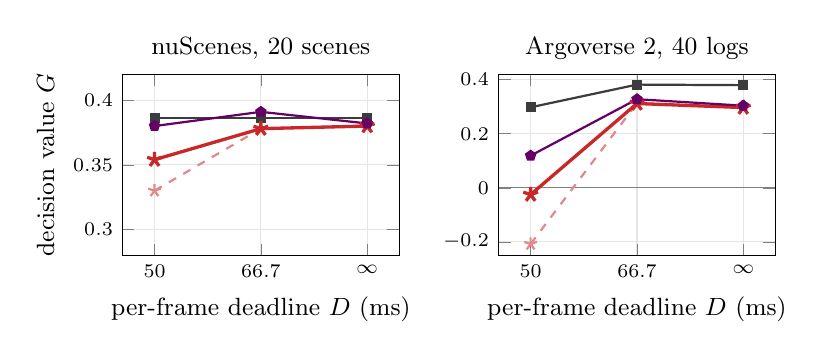
\begin{tikzpicture}
\begin{groupplot}[group style={group size=2 by 1, horizontal sep=36pt},
  width=0.42\linewidth, height=0.32\linewidth, xmin=-0.3, xmax=2.3, xtick={0,1,2},
  xticklabels={50, 66.7, $\infty$}, xlabel={per-frame deadline $D$ (ms)}, tick label style={font=\scriptsize},
  label style={font=\small}, title style={font=\small, yshift=-4pt}, grid=major, grid style={gray!20},
  yticklabel style={/pgf/number format/fixed, /pgf/number format/precision=2},
  legend style={font=\scriptsize, draw=gray!50, column sep=4pt}, legend cell align=left]
\nextgroupplot[title={nuScenes, 20 scenes}, ymin=0.28, ymax=0.42, ylabel={decision value $\G$}, legend to name=dllegend, legend columns=4]
\draw[black!50, thin] (axis cs:-0.3,0) -- (axis cs:2.3,0);
\addplot[unic, thick, mark=square*, mark size=1.4pt] coordinates {(0,0.386) (1,0.386) (2,0.386)};
\addlegendentry{u960 + comp.\ (hold)}
\addplot[oursc!55, thick, dashed, mark=star, mark size=2.4pt, mark options={solid}] coordinates {(0,0.330) (1,0.378) (2,0.380)};
\addlegendentry{\method (hold)}
\addplot[oursc, very thick, mark=star, mark size=2.8pt] coordinates {(0,0.354) (1,0.378) (2,0.380)};
\addlegendentry{\method, in-loop}
\addplot[violet!80!black, thick, mark=pentagon*, mark size=1.7pt] coordinates {(0,0.380) (1,0.391) (2,0.382)};
\addlegendentry{bounded-keep, in-loop}
\nextgroupplot[title={Argoverse~2, 40 logs}, ymin=-0.25, ymax=0.42]
\draw[black!50, thin] (axis cs:-0.3,0) -- (axis cs:2.3,0);
\addplot[unic, thick, mark=square*, mark size=1.4pt] coordinates {(0,0.298) (1,0.382) (2,0.380)};
\addplot[oursc!55, thick, dashed, mark=star, mark size=2.4pt, mark options={solid}] coordinates {(0,-0.208) (1,0.313) (2,0.297)};
\addplot[oursc, very thick, mark=star, mark size=2.8pt] coordinates {(0,-0.025) (1,0.312) (2,0.297)};
\addplot[violet!80!black, thick, mark=pentagon*, mark size=1.7pt] coordinates {(0,0.119) (1,0.328) (2,0.304)};
\end{groupplot}
\end{tikzpicture}

\vspace{2pt}
\pgfplotslegendfromname{dllegend}
\caption{\textbf{Decision value under per-frame deadlines}, run in the loop on the Jetson AGX Xavier (nuScenes: $20$ test scenes; Argoverse~2: $40$ test logs; three repetitions). Hold: a late action is replaced by the last action that was on time. In-loop: the loop stops before a round that would exceed the deadline and returns the action of the last completed round, and a frame that is still late is held. Bounded-keep: at most two crop batches after the draft, keeping pending truncated detections. Decision values on these subsets, not on the full test splits; values and late shares in \cref{tab:deadline}.}
\label{fig:deadline}
\end{figure}

\Cref{tab:deadline} runs the pipelines on the Jetson under per-frame deadlines, each with its own history; the rule for stopping the loop and the $40$ Argoverse~2 logs were fixed before the run, and without a deadline the actions equal those of \cref{tab:latency} on every common frame.
Stopping the loop before a round that would exceed the deadline is better than holding a late action (Argoverse~2, $50$\,ms: $+0.18$ $\ci{+0.03}{+0.36}$), and bounded-keep retains its decision value from $50$\,ms on nuScenes and from $66.7$\,ms on Argoverse~2.
Whole-frame inference at $960$ pixels with the components runs a single engine pass with a lower tail latency on this device ($95$th percentile $31$ and $47$\,ms), so that it is rarely late; it matches \method on nuScenes and leads on Argoverse~2 ($0.30$ \vs $0.12$ at $50$\,ms and $0.38$ \vs $0.33$ at $66.7$\,ms, not significant) with $4$--$5\times$ its pixels.
Without a deadline, \method attains $0.297$ and u960 with the components $0.380$ on the $40$ logs, the ordering of the full Argoverse~2 split, whereas the $8$ logs of \cref{tab:latency} give the opposite ordering; the timed subsets therefore differ in their relative decision values.

% --- Table: latency-decision frontier (handoff/K39/k39_1_rows.csv, k39_1_deadline.csv, k39_1_diffs.csv, parity.json) ---
\begin{table}[!htbp]
\centering
\caption{\textbf{Latency--decision frontier on the Jetson AGX Xavier} under per-frame deadlines $D$, on the frames of \cref{fig:deadline}, three repetitions in one session per repetition, in rotated order. The fixed-shape engines replay CUDA graphs, which leaves every action, crop, and pixel count unchanged. px: detector-input pixels in \% of the native frame; p95: $95$th-percentile latency without a deadline (ms). Whole frame and hybrid hold a late action; \method stops the loop in time (in-loop). Hybrid: support + ego-corridor tube with the components under the nominal cap at the pixels of \method. $^{\ddagger}$: on the dynamic engine. The one-batch variant was added after the other results were known.}
\label{tab:frontier}
\small
\setlength{\tabcolsep}{2.6pt}
\begin{tabular}{@{}lccccccccccccc@{}}
\toprule
 & \multicolumn{6}{c}{nuScenes, $20$ test scenes} & & \multicolumn{6}{c}{Argoverse~2, $40$ test logs} \\
\cmidrule(lr){2-7}\cmidrule(l){9-14}
 & & & \multicolumn{4}{c}{$\G$ at $D$ (ms)} & & & & \multicolumn{4}{c}{$\G$ at $D$ (ms)} \\
\cmidrule(lr){4-7}\cmidrule(l){11-14}
Pipeline & px & p95 & $33.3$ & $50$ & $66.7$ & $\infty$ & & px & p95 & $33.3$ & $50$ & $66.7$ & $\infty$ \\
\midrule
Cheap (u320) & 4.3 & 7.7 & 0.000 & 0.000 & 0.000 & 0.000 & & 2.6 & 10.1 & 0.000 & 0.000 & 0.000 & 0.000 \\
u512 + comp. & 10.2 & 21.4 & 0.351 & 0.336 & 0.336 & 0.336 & & 6.7 & 36.3 & $-$0.095 & 0.361 & 0.361 & 0.358 \\
u640 + comp. & 17.1 & 23.5 & 0.345 & 0.330 & 0.330 & 0.330 & & 10.3 & 38.9 & 0.139 & 0.367 & 0.375 & 0.373 \\
u800 + comp.$^{\ddagger}$ & 26.7 & 28.6 & 0.414 & 0.369 & 0.369 & 0.369 & & 15.3 & 43.3 & $-$0.300 & 0.383 & 0.383 & 0.381 \\
u960 + comp. & 38.4 & 29.1 & 0.423 & 0.386 & 0.386 & 0.386 & & 23.2 & 45.2 & $-$0.692 & 0.352 & 0.382 & 0.380 \\
u1280 + comp. & 65.4 & 34.8 & 0.434 & 0.410 & 0.395 & 0.395 & & 40.0 & 53.1 & $-$1.649 & 0.119 & 0.408 & 0.400 \\
Native + comp. & 103.1 & 43.7 & $-$8.024 & 0.364 & 0.364 & 0.364 & & 101.2 & 83.3 & $-$1.649 & $-$1.649 & $-$1.647 & 0.147 \\
\midrule
Hybrid, capped & 10.3 & 73.1 & $-$0.280 & 0.153 & 0.196 & 0.373 & & 7.3 & 96.8 & $-$0.726 & $-$0.279 & $-$0.089 & 0.296 \\
\oursrow \textbf{\method} & 7.4 & 55.1 & $-$0.204 & 0.354 & 0.378 & 0.380 & & 5.3 & 74.3 & 0.000 & 0.213 & 0.315 & 0.297 \\
\oursrow \textbf{\method}, bounded-keep & 7.8 & 46.8 & 0.290 & 0.383 & 0.391 & 0.382 & & 5.9 & 63.8 & $-$0.241 & 0.130 & 0.336 & 0.304 \\
\method, one batch, keep (post hoc) & 6.2 & 32.8 & 0.437 & 0.400 & 0.391 & 0.391 & & 4.2 & 44.6 & $-$0.148 & 0.277 & 0.269 & 0.269 \\
\bottomrule
\end{tabular}
\end{table}

\noindent\textbf{Latency--decision frontier.}
\Cref{tab:frontier} repeats the deadline experiment with more whole-frame resolutions, the capped hybrid, and CUDA-graph replay of the fixed-shape engines, which shortens all pipelines; without a deadline, the actions, crops, and pixels of \method and of bounded-keep equal those of the earlier run on every timed frame.
Since the deadlines lie close to the latencies, individual values under a deadline differ from \cref{fig:deadline}; u960 with the components again matches \method on nuScenes and leads on Argoverse~2.
Whole-frame inference at $512$ to $960$ pixels is a strong baseline on this device: it runs a single engine pass, is rarely late, and on Argoverse~2 attains a higher decision value than \method and bounded-keep at every deadline from $50$\,ms ($0.35$--$0.38$ \vs $0.13$--$0.34$), significantly only at $50$\,ms against u800 ($-0.170$, $\ci{-0.312}{-0.015}$) and against u960 on the dynamic engine.
On nuScenes, \method and bounded-keep do not differ significantly from whole-frame inference at any resolution from $50$\,ms, except that both are significantly better than u640 at some deadlines, while at $33.3$\,ms both are significantly worse than whole-frame inference at $800$ to $1280$ pixels.
With the same nominal pixels, the hybrid has a $95$th-percentile latency of $73$ and $97$\,ms, and \method is significantly better than it at $50$\,ms on nuScenes ($+0.201$, $\ci{+0.008}{+0.768}$) and at $33.3$ to $66.7$\,ms on Argoverse~2 ($+0.40$ to $+0.73$).
A variant bounded to a single crop batch, added after these results were known, attains $0.437$ at $33.3$\,ms and $0.400$ at $50$\,ms on nuScenes with $6.2\%$ of the pixels, but only $0.269$ on Argoverse~2; we do not use it elsewhere.
The advantage of \method on this device therefore lies in the decision value per pixel and in the tail latency relative to other crop selection, not in the latency relative to whole-frame inference.

% --- K41-5 / J04 (handoff/K41/J04/k41_5_rows.csv, k41_5_deadline.csv, k41_5_diffs.csv, device_parity; Jetson AGX Xavier, three repetitions) ---
\begin{table}[!htbp]
\centering
\caption{\textbf{All compared methods under per-frame deadlines} on the Jetson AGX Xavier, on the frames of \cref{tab:frontier} (nuScenes: $20$ test scenes; Argoverse~2: $40$ test logs), three repetitions. \method and the iterated methods stop their loop before a round that would exceed the deadline; every other pipeline holds the last action that was on time. p95: $95$th-percentile latency without a deadline (ms). $^{\dagger}$ / $^{\ast}$: \method significantly better / worse ($95\%$ paired interval); $^{\ddagger}$: better also after Holm correction over the rows at that deadline; no row is better than \method after this correction.}
\label{tab:deadline_all}
\footnotesize
\setlength{\tabcolsep}{2.2pt}
\begin{tabular}{@{}lccccccccccccc@{}}
\toprule
 & \multicolumn{6}{c}{nuScenes} & & \multicolumn{6}{c}{Argoverse~2} \\
\cmidrule(lr){2-7}\cmidrule(l){9-14}
 & & \multicolumn{5}{c}{$\G$ at $D$ (ms)} & & & \multicolumn{5}{c}{$\G$ at $D$ (ms)} \\
\cmidrule(lr){3-7}\cmidrule(l){10-14}
Pipeline & p95 & $33.3$ & $50$ & $66.7$ & $100$ & $\infty$ & & p95 & $33.3$ & $50$ & $66.7$ & $100$ & $\infty$ \\
\midrule
Cheap (u320) & 8 & 0.00 & 0.00 & 0.00 & 0.00 & 0.00 & & 10 & 0.00 & 0.00 & 0.00 & 0.00 & 0.00 \\
u512 + comp. & 21 & 0.35$^{\ast}$ & 0.34 & 0.34 & 0.34 & 0.34 & & 36 & $-$0.09 & 0.36$^{\ast}$ & 0.36 & 0.36 & 0.36 \\
u640 + comp. & 23 & 0.35 & 0.33 & 0.33 & 0.33$^{\dagger}$ & 0.33$^{\dagger}$ & & 39 & 0.14 & 0.37$^{\ast}$ & 0.37 & 0.37 & 0.37 \\
u960 + comp. & 29 & 0.42$^{\ast}$ & 0.39 & 0.39 & 0.39 & 0.39 & & 45 & $-$0.78$^{\dagger}$ & 0.35 & 0.38 & 0.38 & 0.38 \\
u1280 + comp. & 35 & 0.43$^{\ast}$ & 0.41 & 0.39 & 0.39 & 0.39 & & 53 & $-$1.6$^{\ddagger}$ & 0.11 & 0.41 & 0.40 & 0.40 \\
Native + comp. & 44 & $-$8.0$^{\dagger}$ & 0.36 & 0.36 & 0.36 & 0.36 & & 83 & $-$1.6$^{\ddagger}$ & $-$1.6$^{\ddagger}$ & $-$1.6$^{\ddagger}$ & 0.15 & 0.15 \\
\midrule
Hybrid, capped & 74 & $-$0.28 & 0.14$^{\ddagger}$ & 0.19 & 0.35 & 0.37 & & 98 & $-$0.84$^{\dagger}$ & $-$0.34$^{\ddagger}$ & $-$0.10$^{\dagger}$ & 0.33 & 0.30 \\
Uncertainty crops, capped & 109 & $-$0.02 & $-$0.25$^{\dagger}$ & 0.05$^{\ddagger}$ & 0.11$^{\ddagger}$ & 0.20 & & 160 & $-$0.98$^{\dagger}$ & $-$0.51$^{\ddagger}$ & $-$0.43$^{\ddagger}$ & 0.12$^{\dagger}$ & 0.19$^{\ddagger}$ \\
\midrule
AdaScale & 51 & $-$8.0$^{\dagger}$ & 0.39 & 0.37 & 0.37 & 0.37 & & 82 & $-$1.6$^{\ddagger}$ & $-$1.6$^{\ddagger}$ & $-$0.92$^{\ddagger}$ & 0.41 & 0.41 \\
Budget-Adaptive Routing & 66 & $-$0.48 & $-$0.47$^{\ddagger}$ & 0.17 & 0.16$^{\dagger}$ & 0.16$^{\dagger}$ & & 97 & $-$1.6$^{\ddagger}$ & $-$0.14$^{\dagger}$ & $-$0.12$^{\ddagger}$ & 0.10$^{\dagger}$ & 0.16$^{\dagger}$ \\
Router, decision-value targets & 44 & $-$1.0 & 0.23 & 0.23$^{\ddagger}$ & 0.23$^{\dagger}$ & 0.23$^{\dagger}$ & & 59 & $-$0.30$^{\dagger}$ & $-$0.03 & 0.22$^{\ddagger}$ & 0.20$^{\ddagger}$ & 0.20$^{\ddagger}$ \\
Chanakya-style policy & 32 & 0.25 & 0.23 & 0.23$^{\ddagger}$ & 0.23$^{\ddagger}$ & 0.23$^{\ddagger}$ & & 47 & $-$0.42 & 0.24 & 0.24 & 0.23$^{\dagger}$ & 0.23$^{\dagger}$ \\
FOVEA, instance saliency & 47 & $-$8.0$^{\dagger}$ & 0.42 & 0.40 & 0.40 & 0.40 & & 67 & $-$1.6$^{\ddagger}$ & $-$1.3$^{\ddagger}$ & 0.23 & 0.37 & 0.37 \\
FOVEA, dataset saliency & 38 & $-$0.27 & $-$0.18 & $-$0.20 & $-$0.20 & $-$0.20 & & 58 & $-$1.6$^{\ddagger}$ & $-$0.16 & 0.31 & 0.33 & 0.33 \\
AnA-style, one pass & 57 & 0.32 & 0.32 & 0.31$^{\dagger}$ & 0.33 & 0.33 & & 111 & $-$1.1$^{\ddagger}$ & $-$0.21 & 0.13 & 0.34 & 0.40 \\
AnA-style, iterated & 67 & 0.32 & 0.32 & 0.31$^{\dagger}$ & 0.33 & 0.33 & & 128 & 0.00 & $-$0.21 & 0.11 & 0.26 & 0.40 \\
Counterfactual, one pass & 38 & $-$0.02 & 0.11 & 0.07$^{\ddagger}$ & 0.07$^{\ddagger}$ & 0.07$^{\ddagger}$ & & 68 & $-$1.5$^{\ddagger}$ & 0.07 & 0.28 & 0.28 & 0.28 \\
Counterfactual, iterated & 48 & 0.03 & 0.12 & 0.07$^{\ddagger}$ & 0.07$^{\ddagger}$ & 0.07$^{\ddagger}$ & & 105 & 0.00 & 0.12 & 0.28 & 0.31 & 0.32 \\
\midrule
\oursrow \textbf{\method} & 56 & \textbf{$-$0.19} & \textbf{0.35} & \textbf{0.38} & \textbf{0.38} & \textbf{0.38} & & 75 & \textbf{0.00} & \textbf{0.15} & \textbf{0.31} & \textbf{0.30} & \textbf{0.30} \\
\method, $\le2$ batches & 48 & 0.31 & 0.38 & 0.39 & 0.38 & 0.38 & & 64 & $-$0.35 & 0.10 & 0.34 & 0.31 & 0.30 \\
\method, one batch (post hoc) & 34 & 0.43 & 0.40 & 0.39 & 0.39 & 0.39 & & 45 & $-$0.35 & 0.28 & 0.27 & 0.27 & 0.27 \\
\bottomrule
\end{tabular}
\end{table}

\noindent\textbf{All compared methods under deadlines.}
\Cref{tab:deadline_all} repeats the benchmark of \cref{tab:frontier} with every method of \cref*{M-tab:main}, on the same frames, in one exclusive session of the device.
The actions, pixels, and crops of \method and of the bounded variant equal those of the earlier device runs on every frame, and the actions of all methods agree with their evaluated records on $99.2$--$99.9\%$ of the frames ($96.8$--$100\%$ for the sizes chosen by the routers), the differences coming from the half-precision draft on the device.
No method is significantly better than \method after Holm correction at any deadline, whereas \method is significantly better than $2$ to $5$ methods on nuScenes from $50$\,ms and than $1$ to $8$ on Argoverse~2, mainly those that are too slow for the tighter deadlines.
Without correction, three of the four whole-frame resolutions score higher on nuScenes at $33.3$\,ms, where \method is late on $16\%$ of the frames and stops its loop early on $55\%$, and u512 and u640 score higher on Argoverse~2 at $50$\,ms, where \method is late on $11.5\%$ ($-0.220$, $\ci{-0.404}{-0.011}$ against u640).
On Argoverse~2, whole-frame inference leads \method by $0.05$--$0.10$ from $66.7$\,ms, and AdaScale and AnA-style refinement by up to $0.11$ without a deadline, not significantly.
The variant bounded to one crop batch, added post hoc, is the best variant of \method at $33.3$\,ms on nuScenes ($0.43$) but is worse on Argoverse~2.
Values under a deadline differ slightly from \cref{tab:frontier} (\eg, $0.15$ \vs $0.21$ for \method on Argoverse~2 at $50$\,ms), since the deadlines lie close to the latencies and the runs are separate.
The mean power over the session was $18.6$\,W; since the rows alternate frame by frame, the energy of each row cannot be separated in this run.

\subsection{Controlled closed loop with estimated states}
\label{sec:supp_aeb}

% --- Table: controlled closed loop (handoff/K32/auto/tables/test_summary.csv, g3_primary.csv, g3_primary_intervals.csv, test_intervals_route_seed.csv) ---
\begin{table}[!tbp]
\centering
\caption{\textbf{Controlled closed loop with estimated states} (CARLA, $155$ Bench2Drive routes with braking scenarios, three seeds). Missed: required braking episodes without braking, per route (registered metric); Miss/ev.: share of avoidable required-braking events without braking (\%), the miss rate reported with the onset-delay analysis; Coll. / Avoid.: share of routes (\%) with a collision / an avoidable collision; Delay: mean braking-onset delay (s) relative to privileged perception on avoidable events; Lat.: mean applied latency (ms), measured on the Jetson for the pipeline with its components. L0: no latency; L1: Jetson latency. All pipelines use the geometric lift with the hand-crafted looming estimate and no refiner. $^{\dagger}$ / $^{\ast}$: \method significantly better / worse (paired bootstrap over routes for Missed, over route $\times$ seed for Miss/ev.\ and Delay).}
\label{tab:aeb}
\footnotesize
\setlength{\tabcolsep}{2.4pt}
\begin{tabular}{@{}lccccccccccccc@{}}
\toprule
 & \multicolumn{5}{c}{L0} & & \multicolumn{6}{c}{L1} \\
\cmidrule(lr){2-6}\cmidrule(l){8-13}
Pipeline & Missed & Miss/ev. & Coll. & Avoid. & Delay & & Missed & Miss/ev. & Coll. & Avoid. & Delay & Lat. \\
\midrule
Privileged & 0 & \na & 31.2 & 0.2 & \na & & \na & \na & \na & \na & \na & \na \\
Cheap (u320) & 0.44$^{\dagger}$ & 6.5$^{\dagger}$ & 30.3 & 1.5 & 0.091$^{\dagger}$ & & 0.64$^{\dagger}$ & 10.4$^{\dagger}$ & 33.1 & 3.2$^{\dagger}$ & 0.124$^{\dagger}$ & 7.5 \\
u960 & 0.33 & 2.9 & 30.3 & 1.1 & 0.029$^{\ast}$ & & 0.43 & 4.8$^{\ast}$ & 32.3 & 1.3 & 0.059$^{\ast}$ & 22.7 \\
Native & 0.32 & 3.0 & 31.6 & 1.3 & 0.029$^{\ast}$ & & 0.45 & 4.9$^{\ast}$ & 32.5 & 2.8 & 0.059$^{\ast}$ & 37.9 \\
Uncertainty crops & 0.43$^{\dagger}$ & 5.8$^{\dagger}$ & 31.4 & 1.9 & 0.079$^{\dagger}$ & & 0.62$^{\dagger}$ & 9.8$^{\dagger}$ & 33.1 & 2.6 & 0.130$^{\dagger}$ & 16.1 \\
Support + corridor tube & 0.33 & 3.6 & 32.0 & 1.7 & 0.042 & & 0.47 & 6.7 & 34.4 & 2.2 & 0.081 & 24.1 \\
\method, $\le2$ batches & 0.32 & 3.8 & 31.0 & 1.9 & 0.041 & & 0.45 & 6.3 & 34.8 & 1.9 & 0.078 & 18.3 \\
\midrule
\oursrow \textbf{\method} & 0.29 & 3.7 & 30.1 & 0.6 & 0.040 & & 0.48 & 6.8 & 33.8 & 1.3 & 0.084 & 21.8 \\
\bottomrule
\end{tabular}
\end{table}

Bench2Drive keeps the annotated states of matched objects, so that errors in range and time-to-collision never reach its planner.
We therefore run a controlled closed loop in CARLA~0.9.15 on the $155$ Bench2Drive evaluation routes whose scenarios require braking for vehicles, pedestrians, or bicycles and need no lateral maneuver around an actor, with three traffic seeds.
The PDM-Lite route follower controls the steering and the target speed without seeing any actor, and the braking controller of \cref{sec:supp_metric} acts on the scene of each perception pipeline, with a hold at standstill.
All pipelines use the same YOLOv8s and the geometric lift with the hand-crafted looming estimate, with the time-to-collision taken over $0.5$\,s; the refiner and the learned looming estimate, which were trained on real images, are not used in simulation.
In setting L1, the action of a frame is applied after its latency, drawn from the Jetson measurements of \cref{tab:latency}, for \method conditional on its number of detector calls; uncertainty crops, which were not timed on the device, use a latency model fitted to these measurements (root-mean-square error $6.6$\,ms on the frames of \method).
As an operational definition for this benchmark, a collision is avoidable unless it is a side or rear impact or the braking demand on the annotated states arises less than $v/6+0.4$\,s before the contact, where $v$ is the ego speed; the latency of L1 is simulated from the measured Jetson latency, not run live.

In \cref{tab:aeb}, most collisions cannot be avoided by longitudinal control, \ie, they are side or rear impacts or late entries into the corridor, as the $31\%$ of the routes with a collision under privileged perception indicate, and no pipeline differs significantly from \method in the collision rate.
\method has the fewest avoidable collisions without latency and as few as u960 with latency, significantly fewer than the cheap detector in this setting.
On avoidable events, \method starts braking significantly earlier than the cheap detector and uncertainty crops, as early as the hybrid, and within $30$\,ms of, but significantly later than, whole-frame inference ($+11$ and $+26$\,ms against u960 in L0 and L1).

\noindent\textbf{Two measures of missed braking.}
The registered measure counts required braking episodes without braking per route; the miss rate counts the share of avoidable required-braking events without braking, paired over route $\times$ seed, and accompanies the onset-delay analysis.
Both rank \method well ahead of the cheap detector and uncertainty crops in L0 and L1.
Against whole-frame inference they agree in L0, where neither difference is significant, but not in L1: per route, \method misses $+0.04$ $\ci{-0.10}{+0.17}$ episodes more than u960 and $+0.02$ $\ci{-0.09}{+0.13}$ more than native-resolution inference, whereas per event its miss rate is higher by $2.0$ percentage points, $\ci{+0.9}{+3.2}$ against u960 and $\ci{+0.8}{+3.3}$ against native-resolution inference.
With latency, \method therefore misses a larger share of avoidable braking events than whole-frame inference, although the per-route count does not resolve the difference; the onset delay of the same events (Delay) points the same way.

\subsection{Planning benchmarks}
\label{sec:supp_planning}

\begin{table}[!htbp]
\centering
\begin{minipage}[t]{0.55\linewidth}
\centering
% --- Table: Bench2Drive (K28 phase3/b2d_v6_summary.csv, three runs; handoff/K30/b2d_summary.csv, inloop_summary.csv) ---
\caption{\textbf{Closed-loop evaluation on Bench2Drive} (219 routes, front-camera perception in the loop). DS, SR: driving score and success rate, mean and standard deviation over three runs; Abil.: mean of the five Multi-Ability success rates; Rec.: recall of the actors within $3$\,s of collision, from a fourth run that logs the perception.}
\label{tab:b2d}
\small
\setlength{\tabcolsep}{2.4pt}
\begin{tabular}{@{}lcccc@{}}
\toprule
Perception & DS & SR & Abil. & Rec.$\,\uparrow$ \\
\midrule
Privileged & $96.6\pm0.2$ & $0.915\pm0.003$ & 0.911 & 1 \\
Cheap (u320) & $92.3\pm0.9$ & $0.834\pm0.018$ & 0.830 & 0.889 \\
u960 & $93.2\pm0.7$ & $0.857\pm0.010$ & 0.855 & 0.845 \\
Native (u1600) & $92.0\pm0.7$ & $0.837\pm0.013$ & 0.839 & 0.897 \\
\oursrow \textbf{\method} & $92.5\pm0.8$ & $0.839\pm0.011$ & 0.833 & 0.906 \\
\bottomrule
\end{tabular}
\end{minipage}\hfill
\begin{minipage}[t]{0.42\linewidth}
\centering
% --- Table: NAVSIM (handoff/K30/pdms_summary_k30m.csv, navtest_summary.csv, navhard_summary.csv) ---
\caption{\textbf{NAVSIM v2} with PDM-Closed and front-camera perception in the loop: EPDMS on navtest ($12{,}146$ scenes) and on the two-stage navhard split.}
\label{tab:navsim}
\small
\setlength{\tabcolsep}{5pt}
\begin{tabular}{@{}lcc@{}}
\toprule
Perception & navtest & navhard \\
\midrule
Privileged (ground truth) & 0.870 & 0.528 \\
Cheap (u320) & 0.862 & 0.508 \\
u960 & 0.864 & 0.508 \\
Native & 0.864 & 0.510 \\
Support + route tube & 0.865 & 0.510 \\
\oursrow \textbf{\method} & 0.865 & 0.509 \\
\bottomrule
\end{tabular}
\end{minipage}
\end{table}

On NAVSIM, an annotated object that projects into the front camera is retained only if it is matched to a detection, and unmatched detections are converted to static objects (\cref{sec:supp_metric}).
Our reference PDM-Closed with ground-truth objects attains $0.900$ on navtest, compared with the published value of $0.881$; its ego-progress sub-score ($0.936$) accounts for most of the difference, but we did not isolate every difference of the setup, which all pipelines share.
On navtest, the scores with the cheap detector and with ground-truth objects differ by $0.007$ PDMS.
The field probed from PDM-Closed attains a PDMS of $0.8945$, compared with $0.8926$ for the closed-form braking field ($\ci{+0.0002}{+0.0040}$).
The two fields differ in shape on $99.8\%$ of the $12{,}146$ scenes (intersection over union below $0.9$; median $0.33$), and $67\%$ of the footprint of the probed field lies outside the braking field, but the selected trajectory differs by more than $0.5$\,m on only $4.3\%$ $\ci{3.6}{4.9}$ of the scenes ($517$).
On these scenes, the probed field improves the PDMS by $0.045$ $\ci{+0.005}{+0.091}$; it scores better on $186$, worse on $265$, and equally on $66$, and the mean gain stems from $35$ scenes whose score changes by $1$, $31$ of them in its favor.
On nuPlan-mini ($1{,}440$ states), whose logs coincide with the NAVSIM development split, \method attains the highest PDMS ($0.940$, compared with $0.937$ for FOVEA and u960, $0.935$ for u640, and $0.933$ for the cheap detector).
\Cref{tab:b2d} reports the closed-loop results on Bench2Drive with CARLA~\cite{carla}, where matched objects retain their true state. One of the $220$ routes is excluded for all pipelines, as the simulator repeatedly fails on it.
Paired over the routes and pooled over the three runs, the driving score of \method does not differ significantly from that of whole-frame inference at the verification resolution ($\ci{-2.20}{+1.03}$) or at the native resolution ($\ci{-1.37}{+2.42}$).
In the logged run, the recall of the actors within $3$\,s of collision is $0.906$ for \method, compared with $0.889$ for the cheap detector and $0.845$ and $0.897$ for whole-frame inference at the verification and the native resolution.
On NAVSIM v2 (\cref{tab:navsim}), all perception pipelines lie within $0.003$ extended PDMS of each other on navtest and within $0.002$ on navhard.
The scenarios in which all perception pipelines fail are accident and construction scenarios, which contain cones and warning signs outside the classes of the COCO-pretrained detector.

\noindent\textbf{Cost of probing the planner.}
On NAVSIM, the field and the support require $50.2$ calls of PDM-Closed per frame on average ($45.1$ probe queries, $4.0$ removal queries, and the base call).
Since the planner input is identical for all calls of a frame, it is constructed once, and the simulated ego roll-outs are reused whenever a query leaves the proposals unchanged, which is the case for $41$ of the $50$ calls; the outputs are identical to those of the reference implementation.
This reduces the cost of a frame by a factor of $11$, to $1.3$\,s at the median and $2.0$\,s at the $95$th percentile with eight CPU worker processes ($6.0$ and $10.1$\,s with one).
Coarser fields reduce the number of calls further without a measurable change of the score: a $5\times5$ grid ($26$ calls), a $3\times3$ grid ($14$ calls), and the cells along the current plan ($15$ calls) change the PDMS on navtest by at most $0.0002$, and all intervals of the difference contain zero; measured on the same $1{,}000$ frames, they take $51\%$, $32\%$, and $33\%$ of the time of the $7\times7$ grid.
For the bottleneck selector of \cref*{M-cor:bottleneck}, an output-identical implementation that caches the base score of each candidate and evaluates only the probe columns reduces the cost of the field and the support from $101.0$ to $11.0$\,ms per frame on one CPU thread for the $7\times7$ grid and from $24.1$ to $6.4$\,ms for the $3\times3$ grid, with identical actions, fields, and supports on all $1{,}000$ frames.
The measured violations of certification by single-object queries are reported in \cref{sec:consumers_outside}.
On Bench2Drive, the field is that of the braking controller and requires no planner query.

\subsection{Planner-anchored crops, PDMS, and interactions on NAVSIM}
\label{sec:supp_navsim_k41}

% --- K41-1 / D04 (handoff/K41/D04/k41_1_d04_summary.csv), P01 (K41/REPORT.md), D07 (K41/D07/), P02 / P03 (K41/k41_2_p02_*.csv, K41/P03/) ---
\begin{table}[!htbp]
\centering
\caption{\textbf{Bottleneck selector on NAVSIM navtest} ($12{,}146$ scenes, real crop detections, official PDMS of NAVSIM v1.1). Agr.: agreement with $\policy(\full)$; Repair: agreement on the $724$ scenes on which the cheap draft differs from $\policy(\full)$, with the interval of \method minus the row; px: crop pixels in the unit of the field. VeteranAD-style rows as in \cref{tab:anchored}, with the $15$ candidates of the selector as anchors. Every interval of the PDMS difference between rows contains zero.}
\label{tab:navsim_k41}
\small
\setlength{\tabcolsep}{3pt}
\begin{tabular}{@{}lccccc@{}}
\toprule
Row & PDMS & Agr. & Repair & $\Delta$ repair & px \\
\midrule
Cheap draft & 0.512 & 0.940 & 0 & \na & \na \\
Reference $\policy(\full)$ & 0.510 & 1 & 1 & \na & \na \\
(a) all anchors & 0.510 & 0.965 & 0.638 & \best{\ci{+0.019}{+0.083}} & 1.26 \\
(b) selected anchors & 0.511 & 0.965 & 0.601 & \best{\ci{+0.057}{+0.124}} & 0.98 \\
(c) selected + support & 0.511 & 0.967 & 0.663 & \ci{-0.004}{+0.058} & 0.84 \\
Support first, then geometric field & 0.511 & 0.968 & 0.674 & \ci{-0.012}{+0.044} & 0.91 \\
Support + route tube & 0.511 & \textbf{0.973} & 0.671 & \na & \na \\
\midrule
\oursrow \textbf{\method} & 0.511 & 0.968 & \textbf{0.689} & \na & 0.83 \\
\bottomrule
\end{tabular}
\end{table}

\noindent\textbf{Agreement is not PDMS.}
For the bottleneck selector of \cref{sec:consumers_outside}, the PDMS of \method ($0.511$, $\ci{0.476}{0.546}$) does not differ significantly from that of the cheap draft ($0.512$) or of the reference ($0.510$): the selector with its $15$ fixed candidates is a weak planner, and its choices with the cheap and the whole-frame detections score alike, so this benchmark tests fidelity, not driving quality.
\Cref{tab:navsim_k41} adds VeteranAD-style crops along the candidates.
\method repairs significantly more disagreements than crops along all candidates or along the selected ones, with fewer pixels, while adding its support to the selected candidates or verifying the support before a geometric field makes the difference not significant.
The hybrid of the support with a fixed tube along the route agrees with $\policy(\full)$ more often than \method ($97.3\%$ \vs $96.8\%$; \method minus hybrid $-0.52$ points, $\ci{-0.76}{-0.27}$) but repairs fewer of the disagreements of the draft ($0.671$ \vs $0.689$).
A field built from pairs of probes ($k=2$) equals the single-probe field of PDM-Closed on all $1{,}000$ scenes of \cref{sec:consumers_outside}, since no pair of adjacent cells changes the plan jointly.

% --- P02 (1,000 scenes) + P03 (remaining 11,146 scenes): bounded-order interaction diagnostics of PDM-Closed ---
\begin{table}[!htbp]
\centering
\caption{\textbf{Joint effects of objects on PDM-Closed} that no single object explains, on the $11{,}146$ navtest scenes not in \cref{sec:consumers_outside} (sampled combinations; a joint effect moves the plan by more than $0.5$\,m within $4$\,s). Rate: share of the tested combinations, with a $95\%$ Wilson interval in the same power of ten; Scenes: share of the scenes with a tested combination that have at least one effect. $\Delta$PDMS: mean change of the PDMS from the base plan to the jointly changed plan, with the numbers of effects that lower / raise it.}
\label{tab:interactions}
\small
\setlength{\tabcolsep}{2.6pt}
\begin{tabular}{@{}lcccc@{}}
\toprule
Family & Effects / tested & Rate & Scenes & $\Delta$PDMS (lower / higher) \\
\midrule
Removal of three objects & $528$ / $166{,}866$ & $3.2\cdot10^{-3}$ \ci{2.9}{3.5} & $2.2\%$ & $-0.33$ ($252$ / $175$) \\
Insertion of two probes & $20$ / $1{,}114{,}600$ & $1.8\cdot10^{-5}$ \ci{1.2}{2.8} & $0.16\%$ & $-0.26$ ($19$ / $1$) \\
Insertion of three probes & $55$ / $1{,}114{,}600$ & $4.9\cdot10^{-5}$ \ci{3.8}{6.4} & $0.32\%$ & $-0.23$ ($50$ / $5$) \\
Adjacent pair of cells & $0$ / $651{,}247$ & $0$ \ci{0}{5.9}$\cdot10^{-6}$ & $0$ & \na \\
\bottomrule
\end{tabular}
\end{table}

\noindent\textbf{Interactions in a general planner.}
\Cref{tab:interactions} extends the measurement of \cref{sec:consumers_outside} to combinations of up to three objects on the remaining navtest scenes, with a fresh instance of PDM-Closed for every scene, at a cost of $337$ CPU hours for $3.1$ million planner calls.
Pairs of adjacent cells never change the plan jointly ($0$ of $709{,}645$ on all scenes), and insertions of two or three probes do so for a few combinations in $10^{5}$.
Removing three objects together changes the plan more often, on $2.2\%$ of the scenes with such triples; this rate per combination is higher than on the first $1{,}000$ scenes ($1.9\cdot10^{-3}$, $\ci{1.3}{2.7}\cdot10^{-3}$), so the smaller sample underestimated it.
When a joint effect occurs, it lowers the PDMS more often than it raises it (mean $-0.32$; on $114$ of the $182$ affected new scenes at least one effect lowers it).
A support from single-object queries therefore misses a small but consequential set of multi-object interactions, and these diagnostics of finite order do not certify the absence of larger ones.

%%%%%%%%%%%%%%%%%%%%%%%%%%%%%%%%%%%%%%%%%%%%%%%%%%%%%%%%%%%%%%%%%%%%%%%%%%%%%%
%% S7. QUALITATIVE RESULTS, FAILURE CASES, REPRODUCIBILITY
%%%%%%%%%%%%%%%%%%%%%%%%%%%%%%%%%%%%%%%%%%%%%%%%%%%%%%%%%%%%%%%%%%%%%%%%%%%%%%
\section{Qualitative results, failure cases, and reproducibility}
\label{sec:supp_qual}

\subsection{Qualitative results}
\label{sec:supp_qualitative}

\Cref*{M-fig:qual} and \cref{fig:qual_n,fig:qual_a1,fig:qual_a2} show frames selected by a fixed rule on the stored test results of the frozen configuration, with categories defined by the actions: unnecessary braking removed (the required action is \textsc{keep}, the cheap pipeline brakes, and \method and u960 with the components keep), range corrected (the cheap detector finds a decision-relevant object, the cheap pipeline and \method without the refiner take an action other than the required one, and \method takes it), missed object recovered by the field (a decision-relevant object is missed by the cheap detector and by the support-only ablation and found by u960 and by \method, which takes the required action), and failure (\method takes an action other than the required one and u960 with the shared components takes it).
Per category and dataset, the first qualifying frame in time order is shown; none is chosen by inspection.

\begin{figure}[p]
\centering
\begin{minipage}{\textwidth}
{\normalsize\textbf{(1) Range corrected}} {\small(nuScenes held-out)}\par\vspace{3pt}
\setlength{\tabcolsep}{2pt}\renewcommand{\arraystretch}{1.0}
\begin{tabular}{@{}cc@{}}
\includegraphics[width=0.492\textwidth]{figs/s_n0289_a.jpg} & \includegraphics[width=0.492\textwidth]{figs/s_n0289_c.jpg} \\
{\footnotesize (a) draft} & {\footnotesize (b) verified crops} \\[3pt]
\includegraphics[width=0.492\textwidth]{figs/s_n0289_d.jpg} & \parbox[b][0.246\textwidth][c]{0.47\textwidth}{\small The draft decelerates for the vehicle ahead. After its verification, the refiner corrects its range, and \method takes the required \textsc{hard-brake}; without the refiner, it decelerates.} \\
{\footnotesize (c) final scene} & \\
\end{tabular}
\end{minipage}
\par\vspace{14pt}
\begin{minipage}{\textwidth}
{\normalsize\textbf{(2) Failure}} {\small(nuScenes held-out)}\par\vspace{3pt}
\setlength{\tabcolsep}{2pt}\renewcommand{\arraystretch}{1.0}
\begin{tabular}{@{}cc@{}}
\includegraphics[width=0.492\textwidth]{figs/s_n0123_a.jpg} & \includegraphics[width=0.492\textwidth]{figs/s_n0123_c.jpg} \\
{\footnotesize (a) draft} & {\footnotesize (b) verified crops} \\[3pt]
\includegraphics[width=0.492\textwidth]{figs/s_n0123_d.jpg} & \parbox[b][0.246\textwidth][c]{0.47\textwidth}{\small The decision-relevant truck lies above the upper edge of the field footprint and is detected neither in the draft nor in the crop. \method keeps \textsc{keep}, whereas u960 with the components decelerates as required.} \\
{\footnotesize (c) final scene} & \\
\end{tabular}
\end{minipage}
\vspace{6pt}
\caption{\textbf{Qualitative results selected by a fixed rule} (nuScenes held-out, the two categories of \mref{fig:qual} not shown there). Blue: draft detections (dashed if replaced) and support crop; dashed red: decision-relevant object missed by the draft; orange: field; grey: guard crops; red: verified detections; green: annotation. Images are cropped to the union of the crops and the decision-relevant objects.}
\label{fig:qual_n}
\end{figure}

\begin{figure}[p]
\centering
\begin{minipage}{\textwidth}
{\normalsize\textbf{(3) Unnecessary braking removed}} {\small(Argoverse~2 val)}\par\vspace{3pt}
\setlength{\tabcolsep}{2pt}\renewcommand{\arraystretch}{1.0}
\begin{tabular}{@{}cc@{}}
\includegraphics[width=0.492\textwidth]{figs/s_a55_a.jpg} & \includegraphics[width=0.492\textwidth]{figs/s_a55_c.jpg} \\
{\footnotesize (a) draft} & {\footnotesize (b) verified crops} \\[3pt]
\includegraphics[width=0.492\textwidth]{figs/s_a55_d.jpg} & \parbox[b][0.246\textwidth][c]{0.47\textwidth}{\small The draft decelerates for the car on the right. The support crop verifies it, and with the refined range, \method takes the required \textsc{keep}.} \\
{\footnotesize (c) final scene} & \\
\end{tabular}
\end{minipage}
\par\vspace{14pt}
\begin{minipage}{\textwidth}
{\normalsize\textbf{(4) Range corrected}} {\small(Argoverse~2 val)}\par\vspace{3pt}
\setlength{\tabcolsep}{2pt}\renewcommand{\arraystretch}{1.0}
\begin{tabular}{@{}cc@{}}
\includegraphics[width=0.492\textwidth]{figs/s_a34_a.jpg} & \includegraphics[width=0.492\textwidth]{figs/s_a34_c.jpg} \\
{\footnotesize (a) draft} & {\footnotesize (b) verified crops} \\[3pt]
\includegraphics[width=0.492\textwidth]{figs/s_a34_d.jpg} & \parbox[b][0.246\textwidth][c]{0.47\textwidth}{\small The draft detects the painted bicycle symbol as an object and brakes hard. The verification re-detects it, the refiner corrects its range, and \method takes the required \textsc{decelerate}.} \\
{\footnotesize (c) final scene} & \\
\end{tabular}
\end{minipage}
\vspace{6pt}
\caption{\textbf{Qualitative results selected by a fixed rule} (Argoverse~2 val). Blue: draft detections (dashed if replaced) and support crop; dashed red: decision-relevant object missed by the draft; orange: field; grey: guard crops; red: verified detections; green: annotation. Images are cropped to the union of the crops and the decision-relevant objects.}
\label{fig:qual_a1}
\end{figure}

\begin{figure}[p]
\centering
\begin{minipage}{\textwidth}
{\normalsize\textbf{(5) Missed object recovered}} {\small(Argoverse~2 val)}\par\vspace{3pt}
\setlength{\tabcolsep}{2pt}\renewcommand{\arraystretch}{1.0}
\begin{tabular}{@{}cc@{}}
\includegraphics[width=0.492\textwidth]{figs/s_a25_a.jpg} & \includegraphics[width=0.492\textwidth]{figs/s_a25_c.jpg} \\
{\footnotesize (a) draft} & {\footnotesize (b) verified crops} \\[3pt]
\includegraphics[width=0.492\textwidth]{figs/s_a25_d.jpg} & \parbox[b][0.246\textwidth][c]{0.47\textwidth}{\small Verifying the field footprint recovers the distant vehicle that the draft misses, and \method takes the required \textsc{decelerate}.} \\
{\footnotesize (c) final scene} & \\
\end{tabular}
\end{minipage}
\par\vspace{14pt}
\begin{minipage}{\textwidth}
{\normalsize\textbf{(6) Failure}} {\small(Argoverse~2 val)}\par\vspace{3pt}
\setlength{\tabcolsep}{2pt}\renewcommand{\arraystretch}{1.0}
\begin{tabular}{@{}cc@{}}
\includegraphics[width=0.492\textwidth]{figs/s_a27_a.jpg} & \includegraphics[width=0.492\textwidth]{figs/s_a27_c.jpg} \\
{\footnotesize (a) draft} & {\footnotesize (b) verified crops} \\[3pt]
\includegraphics[width=0.492\textwidth]{figs/s_a27_d.jpg} & \parbox[b][0.246\textwidth][c]{0.47\textwidth}{\small Verifying the field footprint recovers the vehicle, but the refined range keeps the action at \textsc{keep}, where \textsc{decelerate} is required; without the refiner, \method decelerates.} \\
{\footnotesize (c) final scene} & \\
\end{tabular}
\end{minipage}
\vspace{6pt}
\caption{\textbf{Qualitative results selected by a fixed rule} (Argoverse~2 val, continued). Blue: draft detections (dashed if replaced) and support crop; dashed red: decision-relevant object missed by the draft; orange: field; grey: guard crops; red: verified detections; green: annotation. Images are cropped to the union of the crops and the decision-relevant objects.}
\label{fig:qual_a2}
\end{figure}

\subsection{Failure modes}
\label{sec:supp_failures}

\Cref{tab:failures} summarizes the principal failure modes and points to the analyzes that support them.

\begin{table}[!htbp]
\centering
\caption{\textbf{Failure modes of \method} and where they are measured.}
\label{tab:failures}
\small
\renewcommand{\arraystretch}{1.15}
\begin{tabular}{@{}p{4.3cm}p{9.4cm}p{1.6cm}@{}}
\toprule
Failure mode & Evidence & Section \\
\midrule
Decisive object outside the verified region & Coverage $0.92$--$0.96$; lowest for objects more than $3$\,m from the ego lane, for objects that the draft misses, and for the fastest-closing third on nuScenes ($0.80$), which the static probe does not anticipate; example~(2) & \ref{sec:supp_coverage}, \ref{sec:supp_qualitative} \\
Decisive object verified, but its state estimated inaccurately & Of the $60$ costliest frames in which \method brakes less than required, $46$ have a detected decisive object with an inaccurate time-to-collision, lateral position, or range, $11$ an object in a crop that is missed, and $3$ an object outside every crop; example~(6) & \ref{sec:theory_practice}, \ref{sec:supp_qualitative} \\
Intermittently verified objects lack looming history & An object that is verified only intermittently lacks the three same-scale observations of the looming estimate and carries no time-to-collision; iterated AnA-style refinement, which verifies every corridor detection on every frame, gives it a continuous history & \ref{sec:supp_config}, \ref{sec:supp_allcomp} \\
Low-confidence draft boxes & $78$ of $117$ natural misses on nuScenes have a draft box with a confidence between $0.05$ and $0.25$, which \method does not verify & \ref{sec:supp_missed} \\
Missed braking below the hard-braking threshold & At the deployed threshold, more missed \textsc{decelerate} episodes than the cheap detector, as for whole-frame inference with the same components, in part through the refiner that all pipelines with the components share; not significant at the constrained threshold & \ref{sec:supp_episodes}, \ref{sec:supp_operating} \\
Classes outside the detector & All perception pipelines fail in the accident and construction scenarios of NAVSIM, which contain cones and warning signs outside the classes of the COCO-pretrained detector & \ref{sec:supp_planning} \\
Tail latency & The re-detections of the truncation guard set the tail; whole-frame inference at $960$ pixels with the components has a lower $95$th percentile and leads under tight deadlines on Argoverse~2 (not significant) & \ref{sec:supp_latency}, \ref{sec:supp_deadline} \\
\bottomrule
\end{tabular}
\end{table}

\subsection{Reproducibility}
\label{sec:supp_repro}

The frozen configuration, the probe grid, the verification loop, the truncation guard, and the training data of the range refiner and the looming estimate are given in \cref{sec:supp_config} and \cref{tab:benchmarks}; the planner, the loss, and all constants in \cref{sec:supp_metric}, and the second planner and the curved corridor in \cref{sec:supp_tube}.
The splits, the selection rule, the configurations evaluated on the test splits, and the two held-out evaluations under protocols fixed in advance are documented in \cref{sec:supp_config,sec:supp_operating,sec:supp_holdout}; the baselines, their candidate grids and selected settings, and the pixel accounting in \cref{sec:supp_baselines,sec:supp_pixels}.
All intervals are paired bootstrap intervals over the units (scenes, logs, sequences, or routes), with $2{,}000$ resamples, a fixed seed, and $95\%$ percentiles; \method is \emph{non-inferior} to a baseline if the lower bound of the difference exceeds $-0.02$, a margin of $2\%$ of the decision loss of the cheap pipeline fixed in advance.
The Jetson timing and deadline protocols are given in \cref{sec:supp_latency,sec:supp_deadline}, the qualitative frames are selected by the rule of \cref{sec:supp_qualitative}, and the plots are generated from the values of \cref{sec:supp_reference}.

%%%%%%%%%%%%%%%%%%%%%%%%%%%%%%%%%%%%%%%%%%%%%%%%%%%%%%%%%%%%%%%%%%%%%%%%%%%%%%
%% REFERENCE TABLES (the two widest tables on landscape pages)
%%%%%%%%%%%%%%%%%%%%%%%%%%%%%%%%%%%%%%%%%%%%%%%%%%%%%%%%%%%%%%%%%%%%%%%%%%%%%%
\begin{landscape}
\section{Reference tables}
\label{sec:supp_reference}

The plots of this document are generated from the following tables, which list the exact values and intervals.
Unless stated otherwise, an interval is the $95\%$ paired bootstrap interval of (\method$\,-\,$method), and an interval in bold lies above zero, \ie, favors \method.

% --- Table: intervals of Table 1 v7 (handoff/K33/table1_v7.csv; native + C1: K28 final/not_above_all.csv and phase2) ---
\begin{table}[!h]
\centering
\caption{\textbf{Intervals for \cref*{M-tab:main}}: decision value $\G$ and $95\%$ paired bootstrap intervals of (\method$\,-\,$method) without a cap ($\Delta$) and with the per-frame cap at the pixels of \method ($\Delta_{\mathrm{cap}}$); bold: above zero; \sw: below zero. The table includes the rows that \cref*{M-tab:main} omits (u640, FOVEA with dataset saliency, and the one-pass variants) and the variants u768, AnA-style refinement with the draft threshold of the other pipelines ($t=0.25$), and the development-best Chanakya-style policy ($^{\S}$: its development pixels exceed those of \method by $17\%$, outside the matching rule).}
\label{tab:main_ci}
\small
\setlength{\tabcolsep}{2.2pt}
\begin{tabular}{@{}lccccccccccc@{}}
\toprule
 & \multicolumn{3}{c}{nuScenes held-out} & & \multicolumn{3}{c}{Argoverse~2 val} & & \multicolumn{3}{c}{Argoverse-HD val} \\
\cmidrule(lr){2-4}\cmidrule(lr){6-8}\cmidrule(l){10-12}
Method & $\G$ & $\Delta$ & $\Delta_{\mathrm{cap}}$ & & $\G$ & $\Delta$ & $\Delta_{\mathrm{cap}}$ & & $\G$ & $\Delta$ & $\Delta_{\mathrm{cap}}$ \\
\midrule
Whole frame, u640 & $-$0.036 & \ci{$-$0.070}{+0.666} & \na &  & 0.311 & \ci{$-$0.076}{+0.035} & \na &  & 0.279 & \best{\ci{+0.026}{+0.329}} & \na \\
Whole frame, u768 & 0.046 & \ci{$-$0.061}{+0.459} & \na &  & 0.308 & \ci{$-$0.080}{+0.043} & \na &  & 0.273 & \best{\ci{+0.032}{+0.336}} & \na \\
Whole frame, u960 & 0.112 & \ci{$-$0.078}{+0.308} & \na &  & 0.338 & \ci{$-$0.102}{+0.004} & \na &  & 0.297 & \best{\ci{+0.017}{+0.320}} & \na \\
Whole frame, u1280 & 0.292 & \ci{$-$0.165}{+0.017} & \na &  & 0.348 & \ci{$-$0.113}{$-$0.005}\sw & \na &  & 0.315 & \best{\ci{+0.013}{+0.278}} & \na \\
Whole frame, native & 0.222 & \ci{$-$0.087}{+0.122} & \na &  & 0.294 & \ci{$-$0.077}{+0.080} & \na &  & 0.430 & \ci{$-$0.048}{+0.028} & \na \\
\midrule
AdaScale & 0.144 & \ci{$-$0.089}{+0.228} & \ci{$-$0.065}{+0.112} &  & 0.341 & \ci{$-$0.107}{+0.002} & \ci{$-$0.040}{+0.099} &  & 0.298 & \best{\ci{+0.017}{+0.319}} & \best{\ci{+0.050}{+0.414}} \\
Budget-Adaptive Routing & 0.169 & \ci{$-$0.032}{+0.125} & \best{\ci{+0.096}{+0.345}} &  & 0.155 & \best{\ci{+0.078}{+0.201}} & \best{\ci{+0.214}{+0.344}} &  & 0.207 & \best{\ci{+0.124}{+0.297}} & \best{\ci{+0.304}{+0.508}} \\
Router, decision-value targets & 0.214 & \ci{$-$0.088}{+0.095} & \best{\ci{+0.094}{+0.339}} &  & 0.189 & \best{\ci{+0.053}{+0.157}} & \best{\ci{+0.216}{+0.328}} &  & 0.011 & \best{\ci{+0.306}{+0.505}} & \best{\ci{+0.313}{+0.516}} \\
Chanakya-style policy & 0.127 & \ci{$-$0.032}{+0.207} & \best{\ci{+0.064}{+0.316}} &  & 0.286 & \ci{$-$0.039}{+0.051} & \best{\ci{+0.193}{+0.309}} &  & 0.297 & \best{\ci{+0.025}{+0.237}} & \best{\ci{+0.290}{+0.497}} \\
Chanakya-style, dev.-best$^{\S}$ & 0.165 & \ci{$-$0.009}{+0.095} & \best{\ci{+0.071}{+0.324}} &  & 0.272 & \ci{$-$0.028}{+0.065} & \best{\ci{+0.198}{+0.311}} &  & 0.310 & \best{\ci{+0.020}{+0.209}} & \best{\ci{+0.285}{+0.490}} \\
\midrule
SAHI & 0.303 & \ci{$-$0.207}{+0.029} & \best{\ci{+0.090}{+0.289}} &  & 0.256 & \ci{$-$0.031}{+0.105} & \best{\ci{+0.246}{+0.424}} &  & 0.229 & \best{\ci{+0.062}{+0.388}} & \best{\ci{+0.166}{+0.430}} \\
FOVEA, instance saliency & 0.150 & \ci{$-$0.049}{+0.179} & \best{\ci{+0.148}{+1.020}} &  & 0.319 & \ci{$-$0.086}{+0.027} & \best{\ci{+0.026}{+0.189}} &  & 0.313 & \best{\ci{+0.016}{+0.278}} & \best{\ci{+0.202}{+0.602}} \\
FOVEA, dataset saliency & 0.161 & \ci{$-$0.061}{+0.197} & \best{\ci{+0.206}{+1.374}} &  & 0.316 & \ci{$-$0.074}{+0.023} & \ci{$-$0.047}{+0.071} &  & 0.312 & \best{\ci{+0.019}{+0.276}} & \best{\ci{+0.222}{+0.677}} \\
UFP & $-$0.058 & \ci{$-$0.030}{+0.670} & \ci{$-$0.065}{+0.243} &  & 0.322 & \ci{$-$0.089}{+0.026} & \ci{$-$0.038}{+0.119} &  & 0.282 & \best{\ci{+0.021}{+0.328}} & \best{\ci{+0.032}{+0.346}} \\
\midrule
AnA-style, one pass & 0.158 & \ci{$-$0.074}{+0.181} & \best{\ci{+0.003}{+0.273}} &  & 0.346 & \ci{$-$0.111}{+0.002} & \ci{$-$0.011}{+0.047} &  & 0.314 & \best{\ci{+0.007}{+0.297}} & \best{\ci{+0.008}{+0.034}} \\
AnA-style, iterated & 0.158 & \ci{$-$0.074}{+0.181} & \best{\ci{+0.001}{+0.270}} &  & 0.349 & \ci{$-$0.113}{$-$0.002}\sw & \ci{$-$0.013}{+0.045} &  & 0.315 & \best{\ci{+0.006}{+0.296}} & \best{\ci{+0.008}{+0.034}} \\
AnA-style, $t=0.25$ & $-$0.037 & \ci{$-$0.014}{+0.470} & \best{\ci{+0.039}{+0.485}} &  & 0.304 & \ci{$-$0.081}{+0.063} & \best{\ci{+0.014}{+0.107}} &  & 0.225 & \best{\ci{+0.036}{+0.396}} & \best{\ci{+0.020}{+0.232}} \\
Counterfactual, one pass & $-$0.091 & \best{\ci{+0.054}{+0.527}} & \best{\ci{+0.049}{+0.524}} &  & 0.245 & \best{\ci{+0.011}{+0.098}} & \best{\ci{+0.016}{+0.101}} &  & 0.307 & \best{\ci{+0.019}{+0.233}} & \best{\ci{+0.008}{+0.222}} \\
Counterfactual, iterated & $-$0.093 & \best{\ci{+0.056}{+0.530}} & \best{\ci{+0.051}{+0.526}} &  & 0.256 & \ci{$-$0.005}{+0.090} & \best{\ci{+0.014}{+0.102}} &  & 0.285 & \best{\ci{+0.033}{+0.253}} & \best{\ci{+0.020}{+0.228}} \\
\midrule
\oursrow \textbf{\method} & 0.211 & \na & \na &  & 0.294 & \na & \na &  & 0.418 & \na & \na \\
\bottomrule
\end{tabular}
\end{table}
\clearpage

% --- Table: whole-frame comparison (handoff/K28 phase2/table_main_{av2,nusc,ahd}_v6.csv) ---
\begin{table}[!h]
\centering
\caption{\textbf{Decision value $\G$ and detector-input pixels (px) of whole-frame inference} (braking controller, identical COCO-pretrained YOLOv8s). ``Plain'': the pipeline as plotted in \cref{fig:gpx}. ``Ref.'': with the range refiner of \method. ``Hand.'' and ``Learn.'': with the refiner and the hand-crafted or the learned looming estimate (``Learn.'' is the shared lift).}
\label{tab:uniform}
\small
\setlength{\tabcolsep}{2.6pt}
\begin{tabular}{@{}lccccccccccccccccc@{}}
\toprule
 & \multicolumn{5}{c}{Argoverse 2} & & \multicolumn{5}{c}{nuScenes} & & \multicolumn{5}{c}{Argoverse-HD} \\
\cmidrule(lr){2-6}\cmidrule(lr){8-12}\cmidrule(l){14-18}
Long side & Plain & Ref. & Hand. & Learn. & px\,(\%) & & Plain & Ref. & Hand. & Learn. & px\,(\%) & & Plain & Ref. & Hand. & Learn. & px\,(\%) \\
\midrule
448 & \na & \na & \na & \na & \na &  & $-$0.026 & 0.011 & 0.073 & 0.086 & 8.0 &  & $-$0.015 & 0.055 & 0.240 & 0.247 & 5.6 \\
512 & $-$0.025 & 0.105 & 0.185 & 0.285 & 6.7 &  & $-$0.003 & 0.039 & 0.093 & 0.124 & 10.2 &  & $-$0.015 & 0.068 & 0.266 & 0.263 & 7.1 \\
640 & $-$0.019 & 0.131 & 0.219 & 0.311 & 10.3 &  & $-$0.166 & $-$0.112 & $-$0.069 & $-$0.036 & 17.1 &  & $-$0.034 & 0.099 & 0.278 & 0.279 & 11.6 \\
960 & $-$0.021 & 0.182 & 0.255 & 0.338 & 23.2 &  & 0.011 & 0.055 & 0.096 & 0.112 & 38.4 &  & $-$0.032 & 0.124 & 0.287 & 0.297 & 25.3 \\
1280 & $-$0.008 & 0.189 & 0.272 & 0.348 & 40.0 &  & 0.201 & 0.251 & 0.269 & 0.292 & 65.4 &  & $-$0.067 & 0.130 & 0.262 & 0.315 & 44.4 \\
1536 & $-$0.031 & 0.168 & 0.233 & 0.328 & 57.3 &  & 0.191 & 0.257 & 0.280 & 0.302 & 92.2 &  & $-$0.075 & 0.130 & 0.268 & 0.357 & 64.0 \\
Native & $-$0.058 & 0.155 & 0.224 & 0.294 & 101.2 &  & 0.121 & 0.176 & 0.197 & 0.222 & 103.1 &  & $-$0.092 & 0.147 & 0.283 & 0.430 & 101.3 \\
\midrule
\method w/o refiner & \multicolumn{4}{c}{0.241} & 5.4 &  & \multicolumn{4}{c}{0.181} & 7.8 &  & \multicolumn{4}{c}{0.422} & 7.0 \\
\oursrow \textbf{\method} & \multicolumn{4}{c}{\textbf{0.294}} & 5.4 &  & \multicolumn{4}{c}{\textbf{0.211}} & 7.8 &  & \multicolumn{4}{c}{\textbf{0.418}} & 7.0 \\
\bottomrule
\end{tabular}
\end{table}
\end{landscape}

\begin{table}[!tbp]
\centering
\caption{\textbf{Intervals for \cref{tab:uniform}}: $95\%$ paired bootstrap intervals of (\method$\,-\,$whole-frame inference with the refiner); bold: above zero; \sw: below zero.}
\label{tab:uniform_ci}
\small
\setlength{\tabcolsep}{2.5pt}
\begin{tabular}{@{}lccc@{}}
\toprule
Long side & Argoverse 2 & nuScenes & Argoverse-HD \\
\midrule
448 & \na & \best{\ci{+0.029}{+0.382}} & \best{\ci{+0.275}{+0.463}} \\
512 & \best{\ci{+0.130}{+0.249}} & \best{\ci{+0.020}{+0.340}} & \best{\ci{+0.274}{+0.445}} \\
640 & \best{\ci{+0.107}{+0.218}} & \best{\ci{+0.026}{+0.725}} & \best{\ci{+0.252}{+0.414}} \\
960 & \best{\ci{+0.056}{+0.167}} & \ci{-0.016}{+0.354} & \best{\ci{+0.198}{+0.418}} \\
1280 & \best{\ci{+0.053}{+0.156}} & \ci{-0.144}{+0.079} & \best{\ci{+0.166}{+0.450}} \\
1536 & \best{\ci{+0.069}{+0.181}} & \ci{-0.188}{+0.128} & \best{\ci{+0.169}{+0.440}} \\
Native & \best{\ci{+0.060}{+0.222}} & \ci{-0.057}{+0.179} & \best{\ci{+0.143}{+0.429}} \\
\bottomrule
\end{tabular}
\end{table}

% --- Table: loss decomposition (handoff/K28/phase3/loss_terms_{nusc,av2,ahd}_v6.csv) ---
\begin{table}[!tbp]
\centering
\caption{\textbf{Decomposition of the decision loss} into insufficient braking (Insuff.), excessive braking (Exc.), and command changes and collisions (Other), each as a share of the total loss of the cheap pipeline; $1-\G$ is the sum of the three. All pipelines except the cheap one use the refiner and the learned looming estimate.}
\label{tab:loss}
\small
\setlength{\tabcolsep}{3.4pt}
\begin{tabular}{@{}lcccccccccccc@{}}
\toprule
 & \multicolumn{3}{c}{nuScenes held-out} & & \multicolumn{3}{c}{Argoverse~2 val} & & \multicolumn{3}{c}{Argoverse-HD val} \\
\cmidrule(lr){2-4}\cmidrule(lr){6-8}\cmidrule(l){10-12}
Pipeline & Insuff. & Exc. & Other & & Insuff. & Exc. & Other & & Insuff. & Exc. & Other \\
\midrule
Cheap (u320) & 0.782 & 0.191 & 0.027 &  & 0.443 & 0.534 & 0.023 &  & 0.192 & 0.793 & 0.015 \\
u960 + comp. & 0.756 & 0.102 & 0.030 &  & 0.437 & 0.205 & 0.020 &  & 0.180 & 0.503 & 0.021 \\
Native + comp. & 0.692 & 0.067 & 0.019 &  & 0.506 & 0.177 & 0.023 &  & 0.182 & 0.367 & 0.022 \\
Uncertainty crops & 0.943 & 0.079 & 0.037 &  & 0.527 & 0.233 & 0.021 &  & 0.279 & 0.421 & 0.018 \\
Support + corridor tube & 0.727 & 0.075 & 0.024 &  & 0.495 & 0.187 & 0.022 &  & 0.187 & 0.386 & 0.019 \\
\midrule
\oursrow \textbf{\method} & 0.696 & 0.071 & 0.022 &  & 0.498 & 0.187 & 0.022 &  & 0.184 & 0.379 & 0.019 \\
\bottomrule
\end{tabular}
\end{table}

% --- Table: attribution of the disagreement with pi(F) (handoff/K28 phase3/attribution_v6.csv, attribution_detail_v6.csv) ---
\begin{table}[!tbp]
\centering
\caption{\textbf{Attribution of the disagreement with $\policy(\full)$} on the test splits (\method without refiner; $\full$: whole-frame inference at the verification resolution with the learned looming estimate). Each row adds one intervention to the row above.}
\label{tab:locality}
\small
\setlength{\tabcolsep}{3pt}
\begin{tabular}{@{}lccc@{}}
\toprule
Setting & nuScenes & Argoverse 2 & Argov.-HD \\
\midrule
\method, crop detections & 0.976 & 0.968 & 0.940 \\
+ reference detections in the crops & 0.984 & 0.980 & 0.953 \\
+ looming estimate of the reference & 0.988 & 0.986 & 0.956 \\
+ closing probe ($10$\,m/s) & 0.991 & 0.989 & 0.963 \\
+ extended grid & 0.992 & 0.993 & 0.968 \\
+ three probe sizes & 0.995 & 0.996 & 0.971 \\
+ limit of ten rounds & 0.995 & 0.996 & 0.971 \\
\bottomrule
\end{tabular}
\end{table}

% --- Table: coverage of the decisive object by the verified region (handoff/K34: coverage_summary.csv; K34-2) ---
\begin{table}[!tbp]
\centering
\caption{\textbf{Coverage of the decisive object} by the verified region of \method (field footprint, support and guard crops accumulated up to the final round) on the frames that require braking, by stratum ($n$: frames). Coverage is box-center geometry, not detection recall. On Argoverse-HD, the annotations do not separate vehicle classes.}
\label{tab:coverage}
\footnotesize
\setlength{\tabcolsep}{2.4pt}
\begin{tabular}{@{}lccccccccc@{}}
\toprule
 & \multicolumn{2}{c}{nuScenes} & & \multicolumn{2}{c}{Argoverse 2} & & \multicolumn{2}{c}{Argoverse-HD} \\
\cmidrule(lr){2-3}\cmidrule(lr){5-6}\cmidrule(l){8-9}
Stratum & Cov. & $n$ & & Cov. & $n$ & & Cov. & $n$ \\
\midrule
All & 0.92 & 928 & & 0.95 & 2{,}854 & & 0.96 & 3{,}593 \\
\midrule
Car & 0.94 & 779 & & 0.97 & 2{,}381 & & \na & \na \\
Truck & 0.83 & 59 & & 0.92 & 152 & & \na & \na \\
Bus & 0.74 & 27 & & 0.81 & 69 & & \na & \na \\
Pedestrian & 0.93 & 29 & & 1.00 & 66 & & 0.98 & 177 \\
Cyclist & 0.65 & 17 & & 0.87 & 62 & & \na & \na \\
Other (AHD: vehicles) & 0.88 & 17 & & 0.89 & 124 & & 0.96 & 3{,}416 \\
\midrule
Range $<20$\,m & 0.91 & 439 & & 0.95 & 1{,}108 & & 0.93 & 716 \\
Range $20$--$40$\,m & 0.93 & 345 & & 0.97 & 1{,}066 & & 0.96 & 1{,}789 \\
Range $40$--$60$\,m & 0.92 & 127 & & 0.94 & 511 & & 0.98 & 783 \\
Range $>60$\,m & 0.88 & 17 & & 0.96 & 169 & & 0.94 & 305 \\
\midrule
Lateral $<1.2$\,m & 0.95 & 560 & & 0.97 & 1{,}588 & & 0.95 & 2{,}505 \\
Lateral $1.2$--$3$\,m & 0.87 & 342 & & 0.95 & 1{,}149 & & 0.97 & 1{,}015 \\
Lateral $>3$\,m & 0.85 & 26 & & 0.83 & 117 & & 0.95 & 73 \\
\midrule
Closing speed, low & 0.99 & 309 & & 0.97 & 952 & & 0.96 & 1{,}198 \\
Closing speed, middle & 0.96 & 309 & & 0.95 & 951 & & 0.95 & 1{,}197 \\
Closing speed, high & 0.80 & 309 & & 0.94 & 951 & & 0.96 & 1{,}198 \\
\midrule
Detected by the draft & 0.93 & 784 & & 0.96 & 2{,}565 & & 0.96 & 2{,}524 \\
Missed by the draft & 0.85 & 144 & & 0.90 & 289 & & 0.97 & 1{,}069 \\
\bottomrule
\end{tabular}
\end{table}

% --- Table: operating curves (handoff/K37/K37-1: k1_points.csv, test splits, post-hoc) ---
\begin{table}[!tbp]
\centering
\caption{\textbf{Operating curves with identical components} on the test splits: missed required episodes and $\G$ at each braking threshold thr$_{\mathrm{decel}}$ (m/s$^2$; deployed: $1.0$). The support + corridor tube receives the per-frame budget of \method at the same threshold.}
\label{tab:curves}
\footnotesize
\setlength{\tabcolsep}{3pt}
\begin{tabular}{@{}lcccccccccccccc@{}}
\toprule
 & \multicolumn{4}{c}{nuScenes held-out (147 episodes)} & & \multicolumn{4}{c}{Argoverse~2 val (190)} & & \multicolumn{4}{c}{Argoverse-HD val (71)} \\
\cmidrule(lr){2-5}\cmidrule(lr){7-10}\cmidrule(l){12-15}
thr$_{\mathrm{decel}}$ & u960 & Native & Tube & \method & & u960 & Native & Tube & \method & & u960 & Native & Tube & \method \\
\midrule
\multicolumn{15}{@{}l}{\emph{Missed episodes} (cheap at $1.0$: $51$, $21$, $12$)} \\
0.6 & 29 & 29 & 36 & 36 & & 13 & 14 & 18 & 19 & & 9 & 10 & 9 & 9 \\
0.8 & 36 & 37 & 45 & 47 & & 20 & 18 & 26 & 27 & & 11 & 15 & 14 & 14 \\
1.0 & 51 & 53 & 58 & 60 & & 31 & 29 & 35 & 36 & & 26 & 27 & 28 & 27 \\
1.2 & 69 & 74 & 78 & 82 & & 46 & 45 & 53 & 50 & & 34 & 36 & 33 & 32 \\
1.5 & 83 & 85 & 89 & 93 & & 64 & 61 & 70 & 74 & & 39 & 41 & 37 & 38 \\
\midrule
\multicolumn{15}{@{}l}{\emph{Decision value $\G$}} \\
0.6 & 0.199 & 0.315 & 0.263 & 0.301 & & 0.415 & 0.365 & 0.378 & 0.376 & & 0.366 & 0.499 & 0.469 & 0.485 \\
0.8 & 0.172 & 0.276 & 0.223 & 0.261 & & 0.391 & 0.347 & 0.344 & 0.343 & & 0.352 & 0.481 & 0.459 & 0.470 \\
1.0 & 0.112 & 0.222 & 0.174 & 0.211 & & 0.338 & 0.294 & 0.296 & 0.294 & & 0.297 & 0.430 & 0.409 & 0.418 \\
1.2 & 0.068 & 0.173 & 0.118 & 0.161 & & 0.276 & 0.221 & 0.223 & 0.216 & & 0.236 & 0.364 & 0.346 & 0.359 \\
1.5 & 0.015 & 0.108 & 0.078 & 0.112 & & 0.146 & 0.094 & 0.072 & 0.068 & & 0.169 & 0.295 & 0.285 & 0.292 \\
\bottomrule
\end{tabular}
\end{table}

% --- Table: latency of the compared methods (handoff/K33/k33j_latency.csv; G: table1_v7.csv, full test splits) ---
\begin{table}[!tbp]
\centering
\caption{\textbf{Latency of the methods of \cref*{M-tab:main}} on the Jetson AGX Xavier (ms, protocol of \cref{tab:latency}, separate runs on the same frames). $\G$ on the full test splits; all methods with the shared components.}
\label{tab:latency_baselines}
\small
\setlength{\tabcolsep}{2.4pt}
\begin{tabular}{@{}lcccccc@{}}
\toprule
 & \multicolumn{3}{c}{nuScenes} & \multicolumn{3}{c}{Argoverse 2} \\
\cmidrule(lr){2-4}\cmidrule(l){5-7}
Method & $\G\uparrow$ & Mean & p95 & $\G\uparrow$ & Mean & p95 \\
\midrule
Cheap (u320) & 0.000 & 7.7 & 8.4 & 0.000 & 10.5 & 11.0 \\
AdaScale & 0.144 & 43.4 & 54.5 & 0.341 & 70.3 & 86.3 \\
Budget-Adaptive Routing & 0.169 & 49.3 & 70.3 & 0.155 & 76.1 & 106.9 \\
Router, decision-value targets & 0.214 & 25.1 & 46.9 & 0.189 & 35.3 & 65.0 \\
Chanakya-style policy & 0.127 & 14.5 & 33.1 & 0.286 & 23.5 & 53.8 \\
SAHI & 0.303 & 84.8 & 96.0 & 0.256 & 153.2 & 172.8 \\
FOVEA, instance saliency & 0.150 & 42.2 & 51.7 & 0.319 & 59.8 & 75.8 \\
FOVEA, dataset saliency & 0.161 & 33.4 & 42.0 & 0.316 & 49.1 & 65.8 \\
UFP & $-$0.058 & 42.7 & 71.9 & 0.322 & 70.9 & 107.8 \\
AnA-style, one pass & 0.158 & 23.7 & 57.8 & 0.346 & 59.6 & 138.5 \\
AnA-style, iterated & 0.158 & 25.4 & 66.9 & 0.349 & 68.3 & 159.6 \\
Counterfactual, one pass & $-$0.091 & 14.6 & 36.9 & 0.245 & 36.4 & 81.1 \\
Counterfactual, iterated & $-$0.093 & 16.3 & 48.1 & 0.256 & 47.8 & 109.3 \\
\midrule
\oursrow \textbf{\method} & 0.211 & 21.5 & 57.4 & 0.294 & 39.8 & 89.1 \\
\bottomrule
\end{tabular}
\end{table}

% --- Table: decision value under deadlines, run in the loop (handoff/K38/K38-1: k38_1_rows.csv, k38_1_diffs.csv; protocol K38-1_protocol.md) ---
\begin{table}[!tbp]
\centering
\caption{\textbf{Decision value under per-frame deadlines} $D$, run on the Jetson AGX Xavier (nuScenes: $20$ test scenes; Argoverse~2: $40$ test logs; three repetitions). In-loop: the loop stops before a round that would exceed $D$ and returns the action of the last completed round; a frame that is still late keeps the last action that was on time (hold), as for u960. At $50$\,ms, u960, \method in-loop, and bounded-keep are late on $0.5$, $6.4$, and $3.9\%$ of the nuScenes and $3.0$, $13.4$, and $19.4\%$ of the Argoverse~2 frames.}
\label{tab:deadline}
\footnotesize
\setlength{\tabcolsep}{2.2pt}
\begin{tabular}{@{}lcccccc@{}}
\toprule
 & \multicolumn{3}{c}{nuScenes} & \multicolumn{3}{c}{Argoverse~2} \\
\cmidrule(lr){2-4}\cmidrule(l){5-7}
Pipeline & $D{=}50$ & $66.7$ & $\infty$ & $50$ & $66.7$ & $\infty$ \\
\midrule
u960 + comp.\ (hold) & 0.386 & 0.386 & 0.386 & 0.298 & 0.382 & 0.380 \\
\method (hold) & 0.330 & 0.378 & 0.380 & $-$0.208 & 0.313 & 0.297 \\
\method, in-loop & 0.354 & 0.378 & 0.380 & $-$0.025 & 0.312 & 0.297 \\
Bounded-keep, in-loop & 0.380 & 0.391 & 0.382 & 0.119 & 0.328 & 0.304 \\
\bottomrule
\end{tabular}
\end{table}

\clearpage
{
\small
\bibliographystyle{ieeenat_fullname}
\bibliography{main}
}

\end{document}
